\chapter{Experiments \& Results} \label{c5:intro}
\thispagestyle{empty}
\epigraph{\itshape Begin at the beginning, the King said gravely, ``and go on till you come to the end: then stop.''}
{---Lewis Carroll, \textit{Alice in Wonderland}}
\section{Passive Learning - Experimental Process}
\label{c5:section_passive_learning}

In Section~\ref{c4:exif_dataset} we have created an EXIF based dataset in three different image orientations (horizontal, vertical, square). Moreover in Section~\ref{c4:dof_dataset} we created the DoF data set from manually annotated horizontal images based on the depth-of-field volume in photos, focusing on a specific photography style.

We experimented on different types of architectures, a simple (SimpleNet) one, a more complex and sophisticated (DenseNet) one and a larger one (VGG16) utilising both of the data sets.
We have followed two training strategies: i) Train a model from scratch, we have used a DenseNet and a SimpleNet architecture ii) Apply transfer learning utilizing a pre-trained VGG16 architecture.

For the two former architectures, we trained the models using a mini-batch size of 32 samples with Adam optimizer and a learning rate $0.0001$.
DenseNet architecture has 3.632 trainable parameters, 8 convolution filters are used for the network's input, with 7$\times$7 kernel size.

DenseNet comprises of repetitive dense blocks and transition layers where the input of a dense block concatenates with its output. After denseblock repetitions a transition layer takes place which feds a 2D Convolution block (BatchNorm-Relu-Conv2D) with the output tensor of the denseblock multiplied by a factor $\theta=0.5$.
Each 2d convolutional layer uses a Glorot uniform kernel initializer~\cite{glorot2010understanding}.
The number of dense blocks set for our architecture is 1 and 2 while the rest of the DenseNet architecture's hyperparameters were based on the original paper implementation~\cite{huang2017densely}.

SimpleNet architecture was inspired from the simplicity of a very deep architecture such VGG using sets of convolution block. It has 4.172 trainable parameters and is constructed with sets of BatchNorm-Relu-Conv2d blocks followed with a max pooling layer. It stacks 5 hidden layers aside from the input layer with 1-1 and 2$\times$ of 2-1 set of convolution blocks-max pooling. The 2D convolution layers use a HeUniform kernel initializer~\cite{he2015delving}.
The first hidden layer has 12 convolution filters used in the receptive field with 12$\times$12 kernel size and 1$\times$1 stride, second and third 5$\times$5 kernel size and the last two, double the convolution filters with 3$\times$3 kernel size.
At the output a global average pooling layers is used before a densely connected layer with 64 nodes and a dropout with 20\% drop rate.

The hyperparameter values above were set after a hyperparameter tuning process on variable set of values in convolution filters, kernel size, hidden-repetition layers and learning rates. For the optimizers Adam\cite{kingma2014adam} was selected among SGD, RMSprop~\cite{hinton2012practical}, Adagrad~\cite{duchi2011adaptive}, Nadam~\cite{dozat2016incorporating} and Adadelta~\cite{zeiler2012adadelta}.

Concerning VGG~\cite{simonyan2014very} architecture, we have initialised the network with imagenet~\cite{krizhevsky2012imagenet} pre-trained weights, removed the last three fully-connected hidden layers and added i) a global average pooling layer, ii) a batch normalization layer and iii) a dense layer with a softmax activation function on two outputs. We froze the pre-trained part of the network and trained the new layers with 2.050 parameters using a mini-batch size of 8 samples with Adam optimizer and learning rate$=0.0001$.

The classifiers have been trained in varying number of epochs until convergence with the following regularization techniques. We have used \textit{early stopping}, monitoring the validation loss for 6 consecutive epochs keeping the best model, to prevent overfitting. 
In addition we have applied a learning rate decay technique, monitoring for 0.0001 delta difference in validation loss for 5 consecutive epochs. When model fitting reaches a learning plateau and the model validation loss does not improve, it reduces the learning rate by a factor of $\times$0.1. 
Worthy noticing we shuffled training set using a buffer size three times the size of its cardinality. 
Images are standardized before the input using the following standardization\footnote{https://www.tensorflow.org/api\_docs/python/tf/image/per\_image\_standardization}.

The experimental framework has been implemented with Tensorflow 2.3, using tf.data.Dataset\footnote{https://www.tensorflow.org/api\_docs/python/tf/data/Dataset} API for data loading and tf.keras.layers\footnote{https://www.tensorflow.org/api\_docs/python/tf/keras/layers} API to build the neural network architectures. Though determinism in deep learning cannot be set alone with static seeds, thus we ensured the reproducibility of the experiments with NVIDIA's determinism framework~\cite{nvidiadet}. Experiments conducted on a workstation with $\text{Intel}^{\textregistered}$ i7 920 3.0GHz, 16Gb RAM and an $\text{NVIDIA}^{\textregistered}$ GTX 1650 4Gb.

\section{Evaluation Metrics}

Our case study falls into a supervised binary classification task, where categorical labels $y_1, \dots, y_n$ are assigned as predefined classes(bokeh-no bokeh or shallow DoF-deep DoF) to a corresponded input sample $x_1, \dots, x_n$ which fed as training examples in a classifier.

The correctness of a binary classifier can be evaluated by computing the number of correctly recognized examples with \textit{bokeh}(true positives), the number of correctly recognized examples without \textit{bokeh}(true negative), the number of examples that were incorrectly assigned as \textit{bokeh}(false positive) and the examples that should have assigned as without \textit{bokeh} but failed(false negatives)~\cite{sokolova2009systematic}. The above, synthesize a confusion matrix that is shown in Table~\ref{c5:cm}, with above categorical labels.


\begin{table}[ht!]
\centering
\begin{tabular}{ll|l|l|}
\cline{3-4}
    &   & \multicolumn{2}{l|}{Predicted} \\ \cline{3-4} 
    &   & Bokeh              & No-Bokeh             \\ \hline
\multicolumn{1}{|c|}{\multirow{2}{*}{\rotatebox[origin=c]{90}{Actual}}} & Bokeh & TP             & FN            \\ \cline{2-4} 
\multicolumn{1}{|c|}{}                        & No-Bokeh & FP             & TN            \\ \hline
\end{tabular}
\caption{Confusion Matrix}
\label{c5:cm}
\end{table}


Classifier performance were measured with the following metrics:
\begin{itemize}
 \item Accuracy, the overall effectiveness of the classifier. $Acc=\frac{tp+tn}{tp+tn+fp+fn}$
 \item F1 score in macro average of the individual class F1 scores. F1 score is the harmonic mean of recall and precision per class and represents a normalized score for general classification performance. ``Macro average'' means that F1 is computed per class and then avaraging them $F1score=\frac{2 * (precision * recall)}{precision + recall} \rightarrow \frac{1}{N} \sum_{i=0}^{N}F1score_i$
 \item Loss, the objective outcome of the loss function $\mathbb{L}$ (categorical cross-entropy), that indicates the classifier's prediction uncertainty.
\end{itemize} 


\section{Passive Learning - Results}

In the following subsections~\ref{c5:exif_results},~\ref{c5:dof_results} we present the evaluation results of the classifier's performance trained on EXIF and DoF based data sets respectively. As expected the accuracy and F1 score are maximised using the DoF manually annotated data set. A discussion is followed along with a brief description introduction in Section~\ref{c5:active_learning}.


\subsection{EXIF dataset - Results}
\label{c5:exif_results}

This Section presents the results for individual classifiers trained with EXIF data sets under three different image orientations. As we have discussed in Section~\ref{c4:exif_samples}, it would be a surprise to observe significant performance from any type of classifier.

\begin{table}[ht!]
\centering
\footnotesize
\begin{tabular}{c|c|c|c|c|c}

\multicolumn{1}{c|}{Architecture} & \multicolumn{1}{c|}{Dataset} & \multicolumn{1}{c|}{Train/Test Accuracy} & \multicolumn{1}{c|}{Train/Test Loss} & \multicolumn{1}{c|}{Train/Test F1} & Epochs/Time\\ \hline

\multirow{3}{*}{DenseNet} & Horizontal & 62.3/59.2 & 0.65/0.65 & 0.62/0.59 & 48/18s\\
                          & Vertical & 60.7/59.1 & 66/66.8 & 60/58.8 & 38/18s\\
                          & \textbf{Square} & \textbf{63.6/63.5} & \textbf{0.64/0.64} & \textbf{63.5/63.5} & 50/100s \\ \hline
\multirow{3}{*}{SimpleNet} & Horizontal & 60.6/58.4 & 0.66/0.67 & 60/58 & 16/65s\\
                          & Vertical & 57.3/57.1 & 0.67/0.67 & 57.3/57.1 & 13/60s\\
                          & \textbf{Square} & \textbf{61/62.9} & \textbf{65.6/64.6} & \textbf{60/62} & 16/382s\\ \hline
\multirow{3}{*}{VGG16}    & Horizontal & 66.9/63.8 & 60.6/66.3 & 66.9/63.8 & 29/144s\\
                          & Vertical & 65.5/59.4 & 0.61/0.70 & 65.5/59.4 & 25/134s\\
                          & \textbf{Square} & \textbf{66/65.1} & \textbf{0.61/0.63} & \textbf{66/65} & 20/790s\\ \hline
\end{tabular}
\caption{Recorder best performance results across all classifiers trained with EXIF.}
\label{c5:exif_results_table}
\end{table}

\begin{figure}[ht!]
    \centering  
    \subfigure{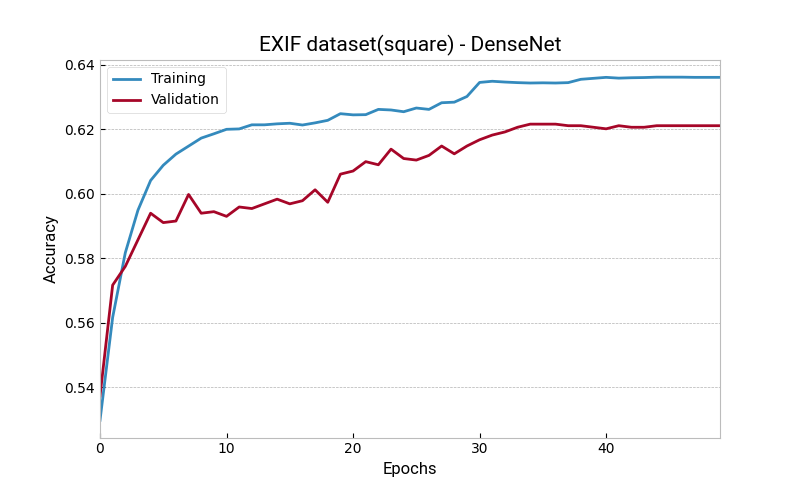
\includegraphics[width=.3\textwidth]{figures/chap5/exif/square-densenetaccuracy}}
    \subfigure{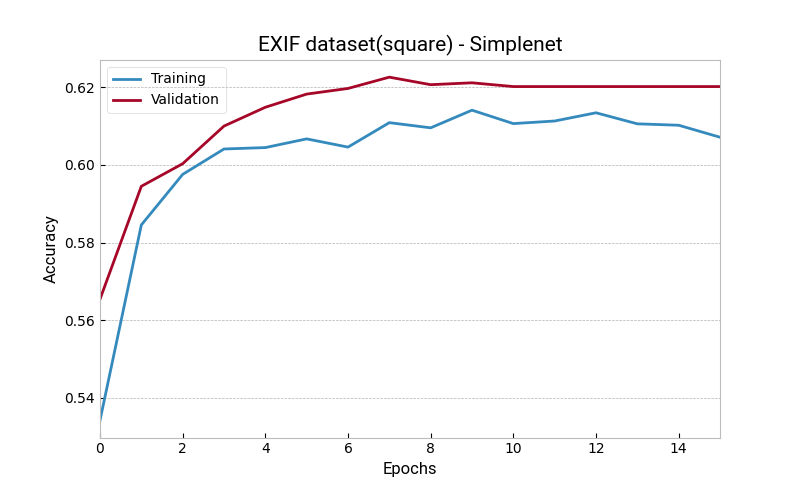
\includegraphics[width=.3\textwidth]{figures/chap5/exif/square-simplenetaccuracy}}
    \subfigure{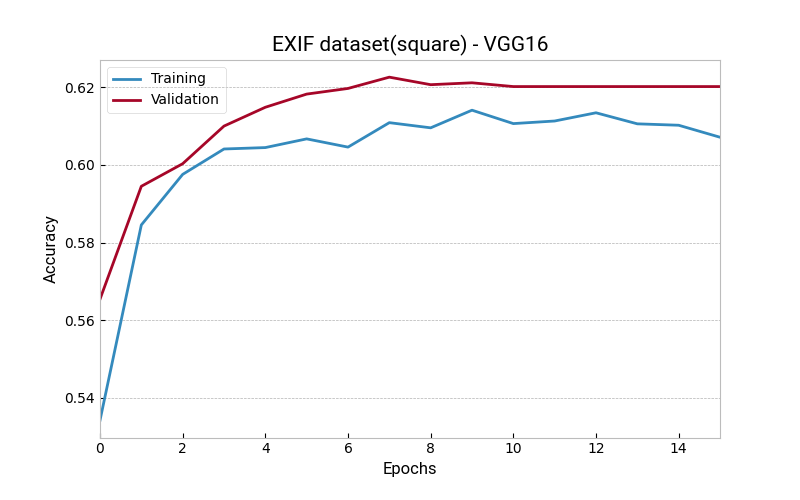
\includegraphics[width=.3\textwidth]{figures/chap5/exif/square-vggaccuracy}}    
    \caption{Training/Validation accuracy history for the total of classifiers trained with EXIF square data set: (a) DenseNet, (b) SimpleNet, (c) VGG16}
    \label{c5:exif_training_history}
\end{figure}

\begin{figure}[ht!]
    \centering  
    \subfigure{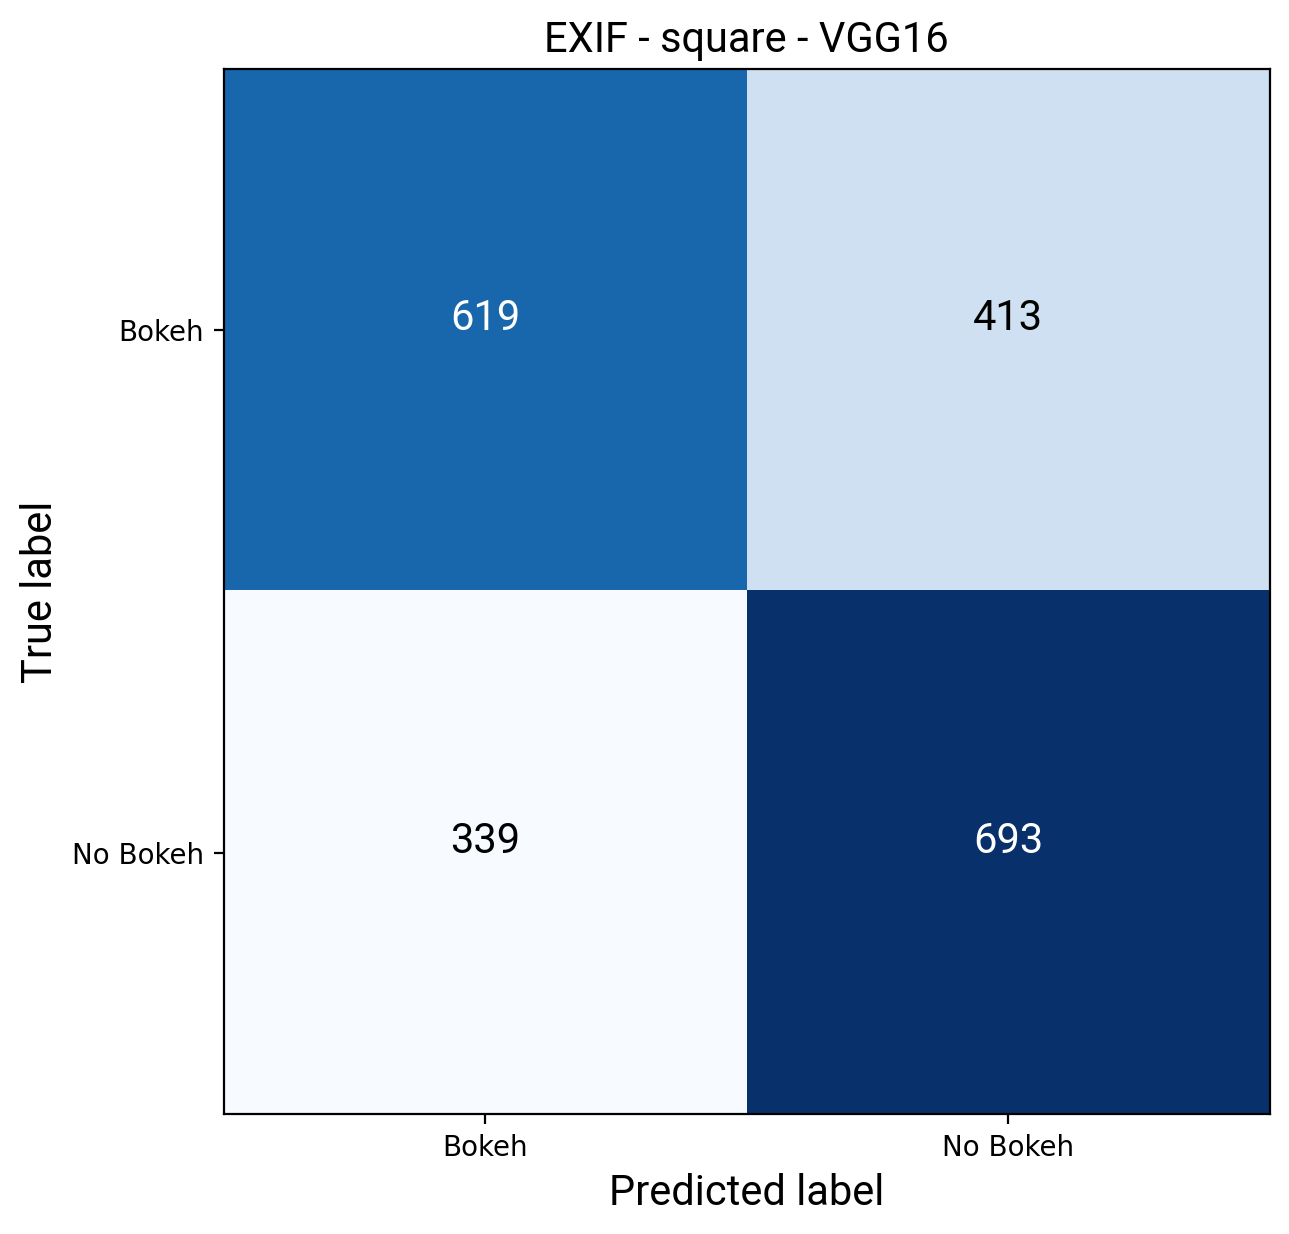
\includegraphics[width=.3\textwidth]{figures/chap5/exif/square-densenetcm}}
    \subfigure{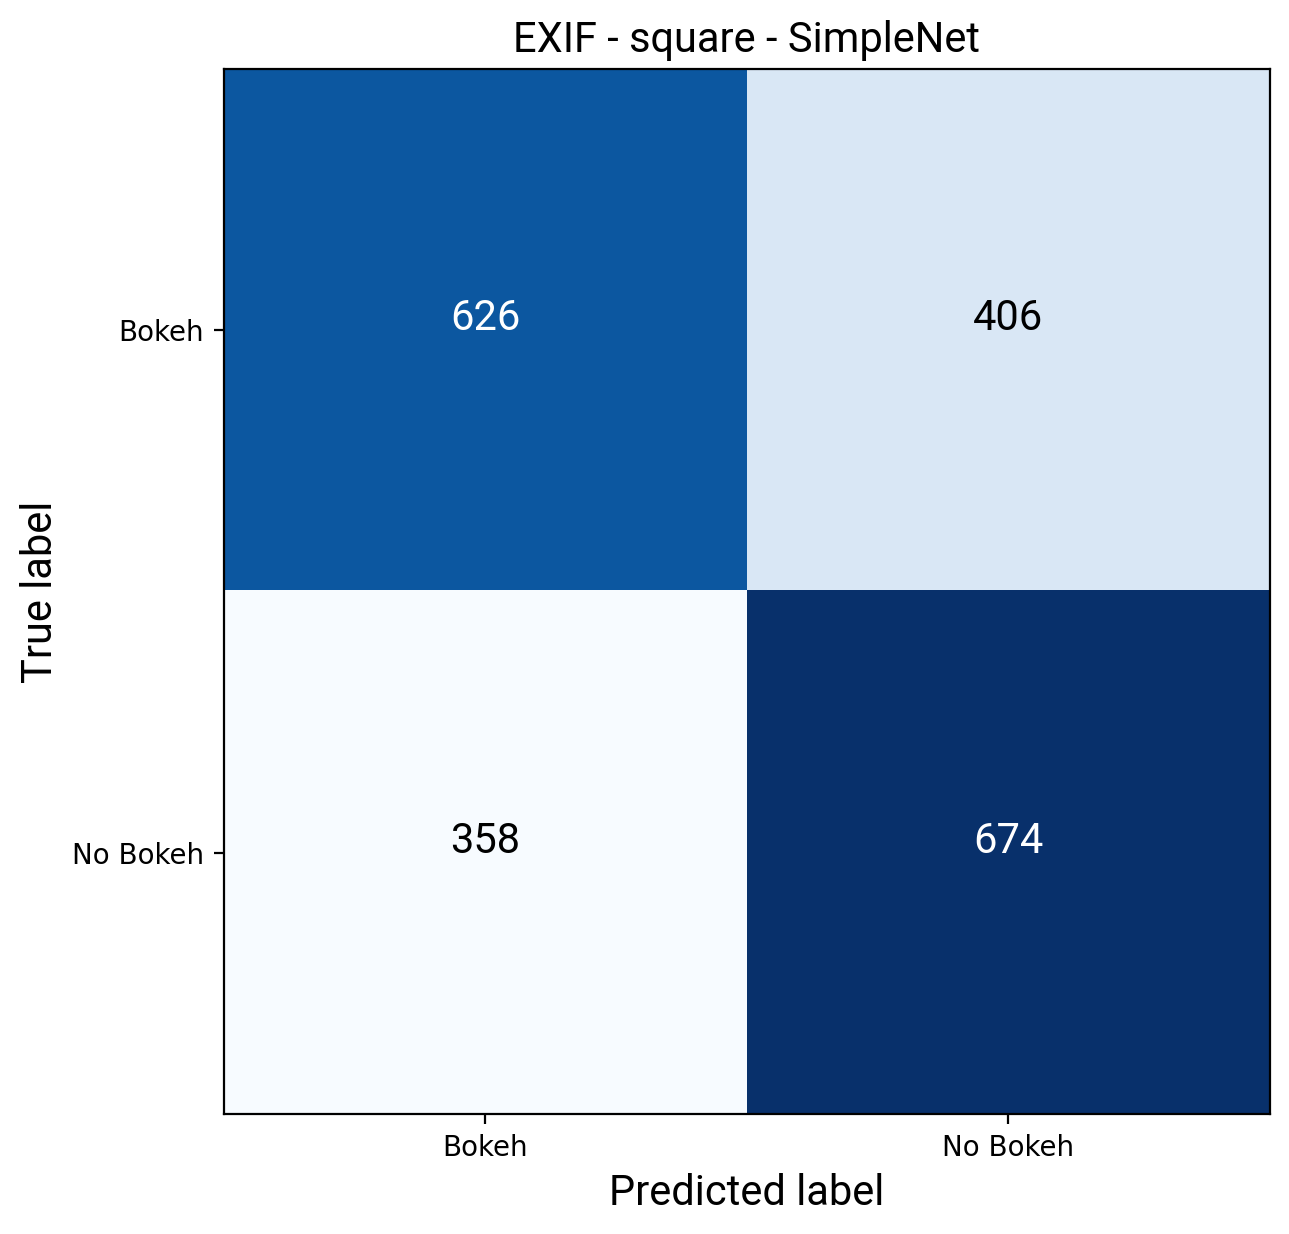
\includegraphics[width=.3\textwidth]{figures/chap5/exif/square-simplenetcm}}
    \subfigure{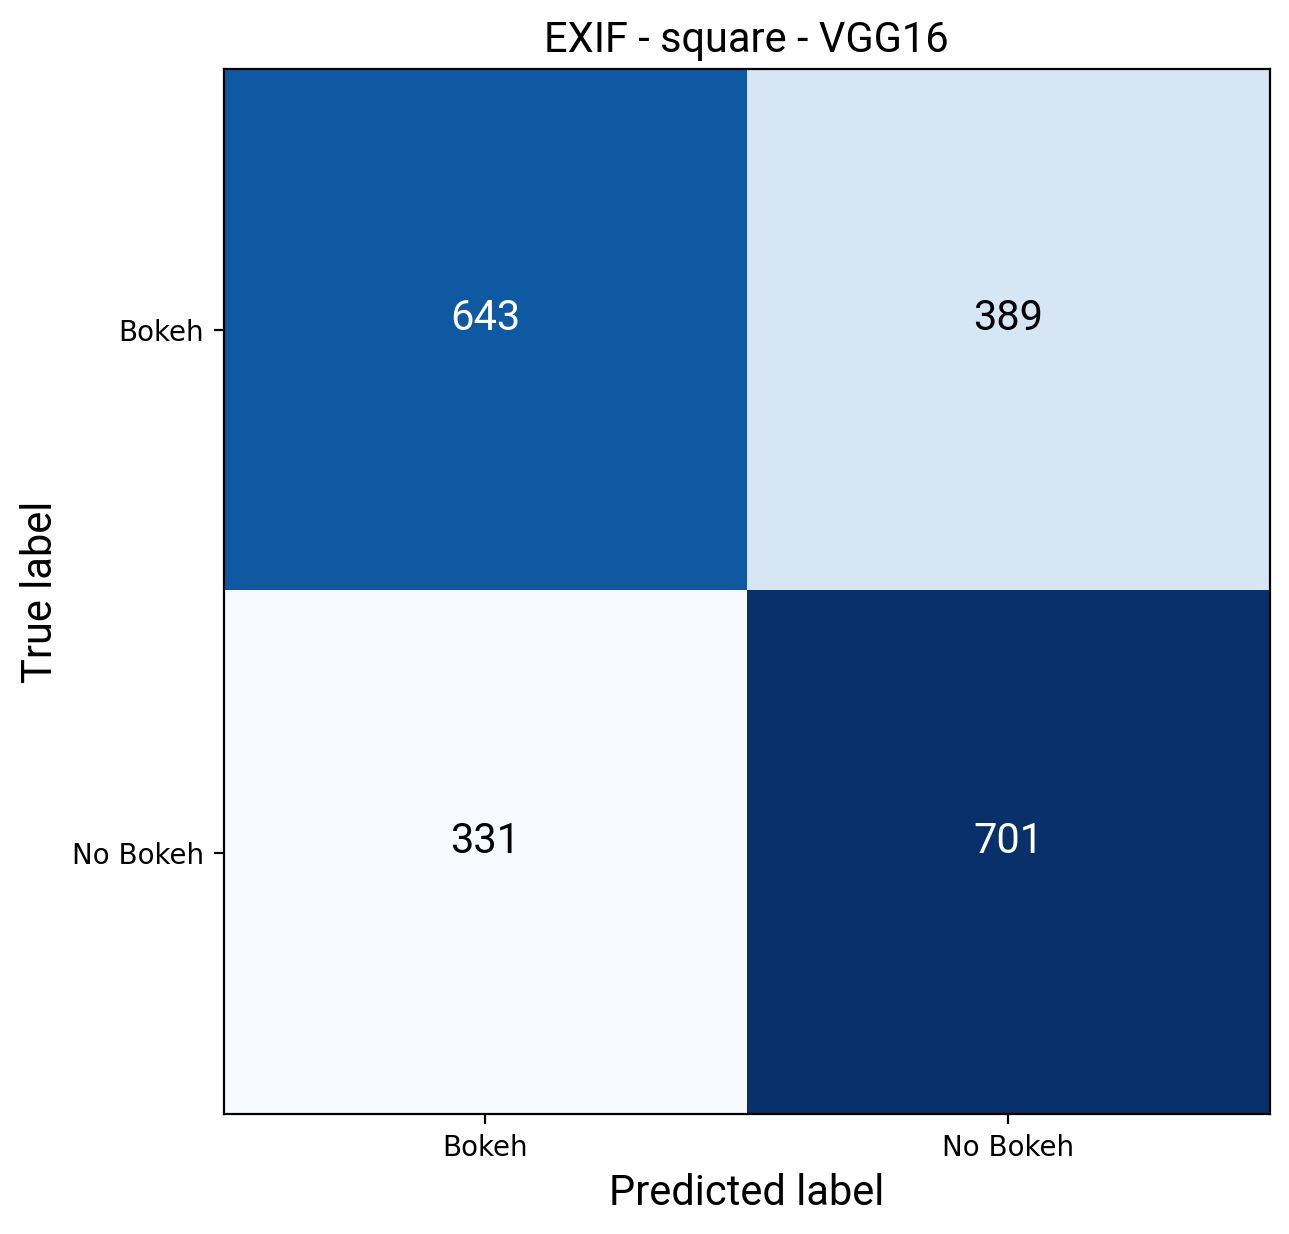
\includegraphics[width=.3\textwidth]{figures/chap5/exif/square-vggcm}}    
    \caption{Confusion matrix for the total of classifiers trained with EXIF square data set: (a) DenseNet, (b) SimpleNet, (c) VGG16}
    \label{c5:exif_cm}
\end{figure}

The results are presented in Table~\ref{c5:exif_results_table} and illustrate the current classifier, the used data set, evaluation metrics, number of epochs and the time in seconds is taken for a complete forward pass.

Concerning the winner classifier, that was the VGG16 which scored 66\% in training set and 65.1\% in testing set. It has been also observed that \textit{squared} dataset offers even $+4\%$ accuracy in comparison with any other dataset. However, this gain is not clear to us if it is due the larger volume of samples or the combined diversity of pictures.

Figure~\ref{c5:exif_training_history} visualise training/validation history for the total of classifiers under the square dataset. It is observed that VGG16 and SimpleNet are overfitting which can be mitigated with a more complex topology. On the other hand, DenseNet presents a regular training curve for a baseline model with minor overfitting.

After a number of experiments, evaluating diverse classifiers under different data set versions, the overall performance is noted within the same range. Since any of the classifiers/data sets does not stand out, it is obvious to us that any hyperparameter tuning cannot can offer a significant boost, since the data set's power is limited.

This led us to generate a human annotated dataset, with categorical labels for shallow/deep depth of field in order to utilize it and train the classifiers.
In the following Section we present the results in training and evaluation of DoF data set which  substantially improves the performance.


\subsection{DoF (annotated) data set - Results}
\label{c5:dof_results}
This Section presents the results for all the classifiers trained with DoF dataset. Table~\ref{c5:dof_results_table} illustrates the performance metrics across the classifiers while Figures~\ref{c5:dof_training_acc_history}-\ref{c5:dof_training_loss_history} visualise the training and validation fitting curves in training history.
Concerning SimpleNet and DenseNet networks, we tuned the models and found the sweet spot, to minimize overfitting as much as possible.
It is clear that VGG16 is again the winner model, but it's worth mentioning that DenseNet based model performs quite close, given the fact that has less capacity, trained from scratch and is 83\% faster in forward pass during training.

\begin{table}[ht!]
\centering
\footnotesize
\begin{tabular}{c|c|c|c|c}

\multicolumn{1}{c|}{Architecture} & \multicolumn{1}{c|}{Train/Test Accuracy} & \multicolumn{1}{c|}{Train/Test Loss} & \multicolumn{1}{c|}{Train/Test F1} & Epochs/Time\\ \hline

DenseNet & 88.3/80.0 & 0.28/0.49 & 88.3/79.9 & 61/2s\\

SimpleNet & 79.4/77.7 & 0.45/0.48 & 79.4/77.7 & 253/6s\\
                        
VGG16 & 94.4/84.1 & 0.19/0.33 & 94.4/84.0 & 75/12s\\

\end{tabular}
\caption{Recorder best performance results across all classifiers trained with DoF(annotated) data set.}
\label{c5:dof_results_table}
\end{table}

\begin{figure}[ht!]
    \centering  
    \subfigure[]{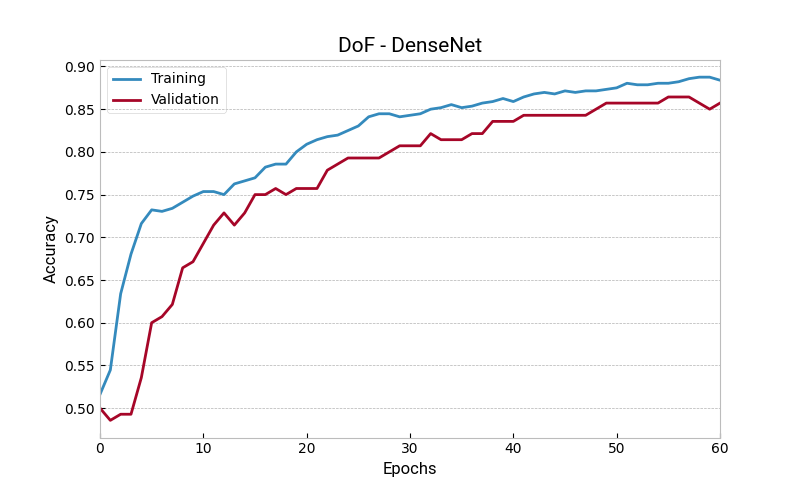
\includegraphics[width=.3\textwidth]{figures/chap5/dof/densenet/accuracy}}
    \subfigure[]{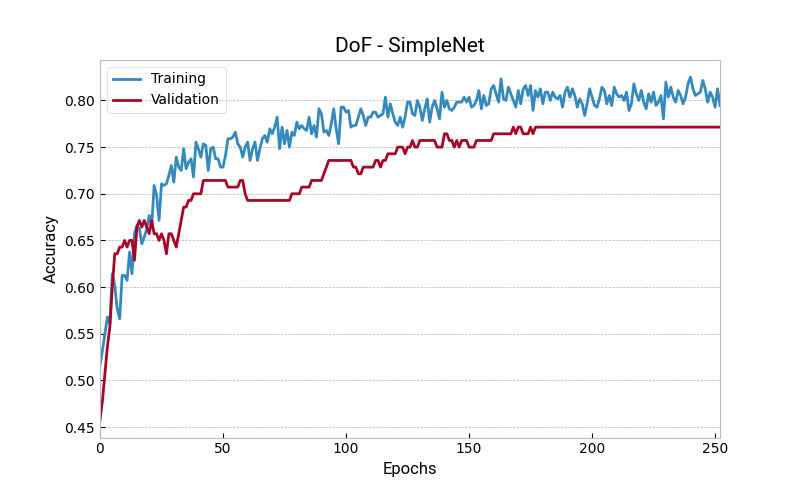
\includegraphics[width=.3\textwidth]{figures/chap5/dof/simplenet/accuracy}}
    \subfigure[]{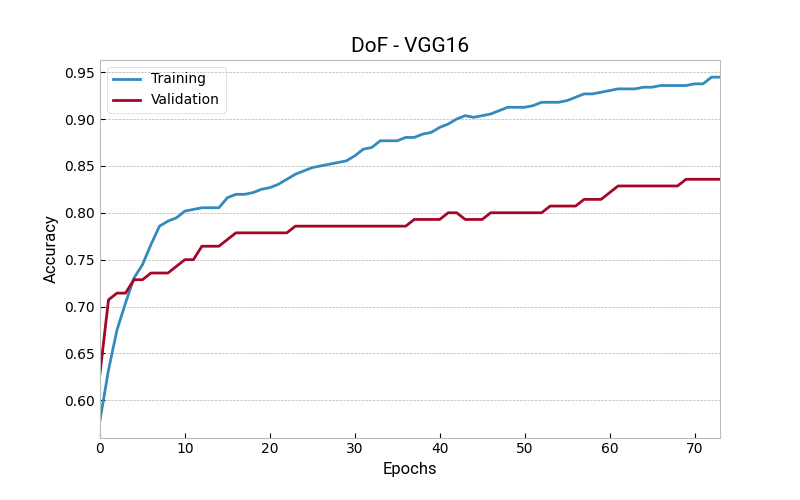
\includegraphics[width=.3\textwidth]{figures/chap5/dof/vgg/accuracy}}
    \caption{Training/Validation accuracy history for the total of classifiers trained with DoF data set: (a) DenseNet, (b) SimpleNet, (c) VGG16}
    \label{c5:dof_training_acc_history}
\end{figure}

\begin{figure}[ht!]
    \centering  
    \subfigure{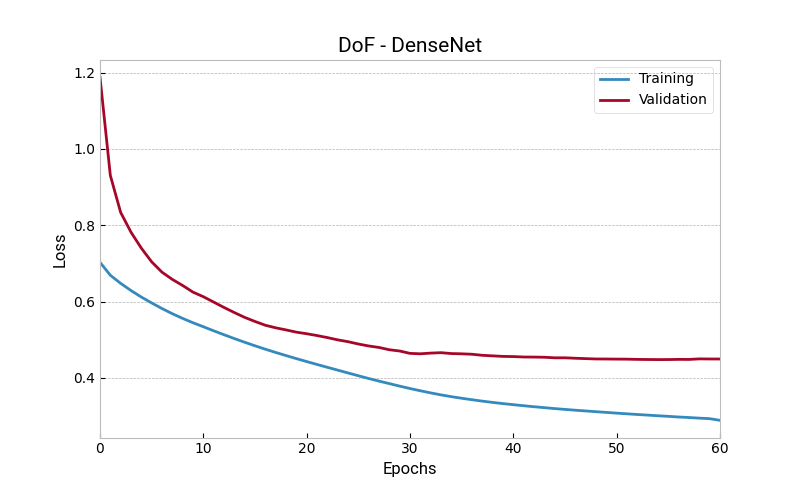
\includegraphics[width=.3\textwidth]{figures/chap5/dof/densenet/loss}}
    \subfigure{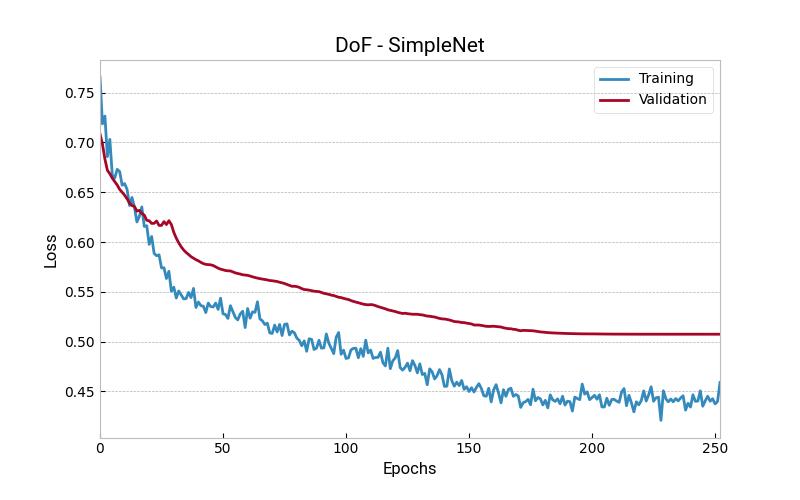
\includegraphics[width=.3\textwidth]{figures/chap5/dof/simplenet/loss}}
    \subfigure{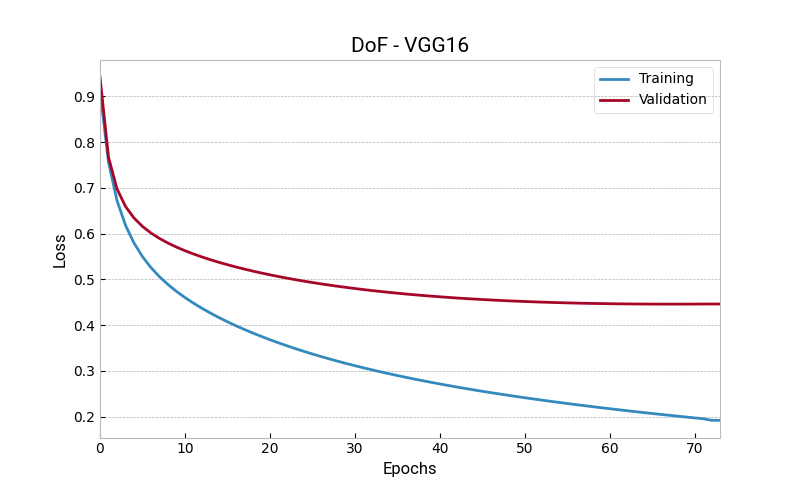
\includegraphics[width=.3\textwidth]{figures/chap5/dof/vgg/loss}}
    \caption{Training/Validation loss history for the total of classifiers trained with DoF data set: (a) DenseNet, (b) SimpleNet, (c) VGG16}
    \label{c5:dof_training_loss_history}
\end{figure}

\begin{figure}[h!]
    \centering  
    \subfigure{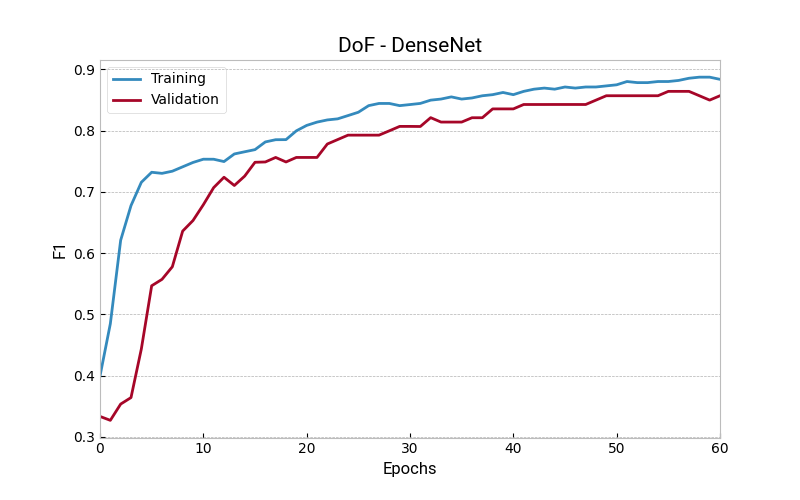
\includegraphics[width=.3\textwidth]{figures/chap5/dof/densenet/f1}}
    \subfigure{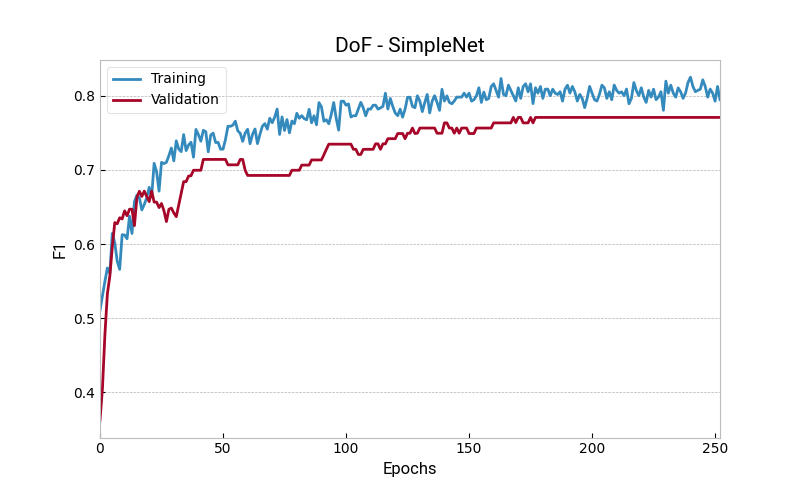
\includegraphics[width=.3\textwidth]{figures/chap5/dof/simplenet/f1}}
    \subfigure{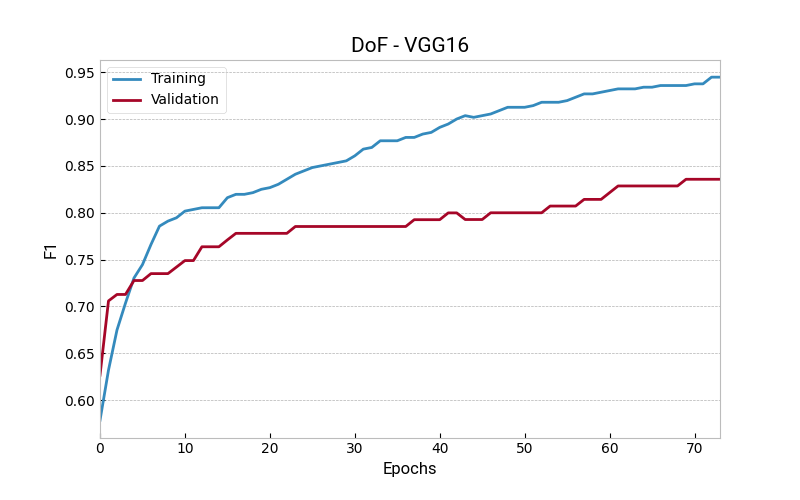
\includegraphics[width=.3\textwidth]{figures/chap5/dof/vgg/f1}}
    \caption{Training/Validation F1-score history for the total of classifiers trained with DoF data set: (a) DenseNet, (b) SimpleNet, (c) VGG16}
    \label{c5:dof_training_f1_history}
\end{figure}

\begin{figure}[ht!]
    \centering  
    \subfigure{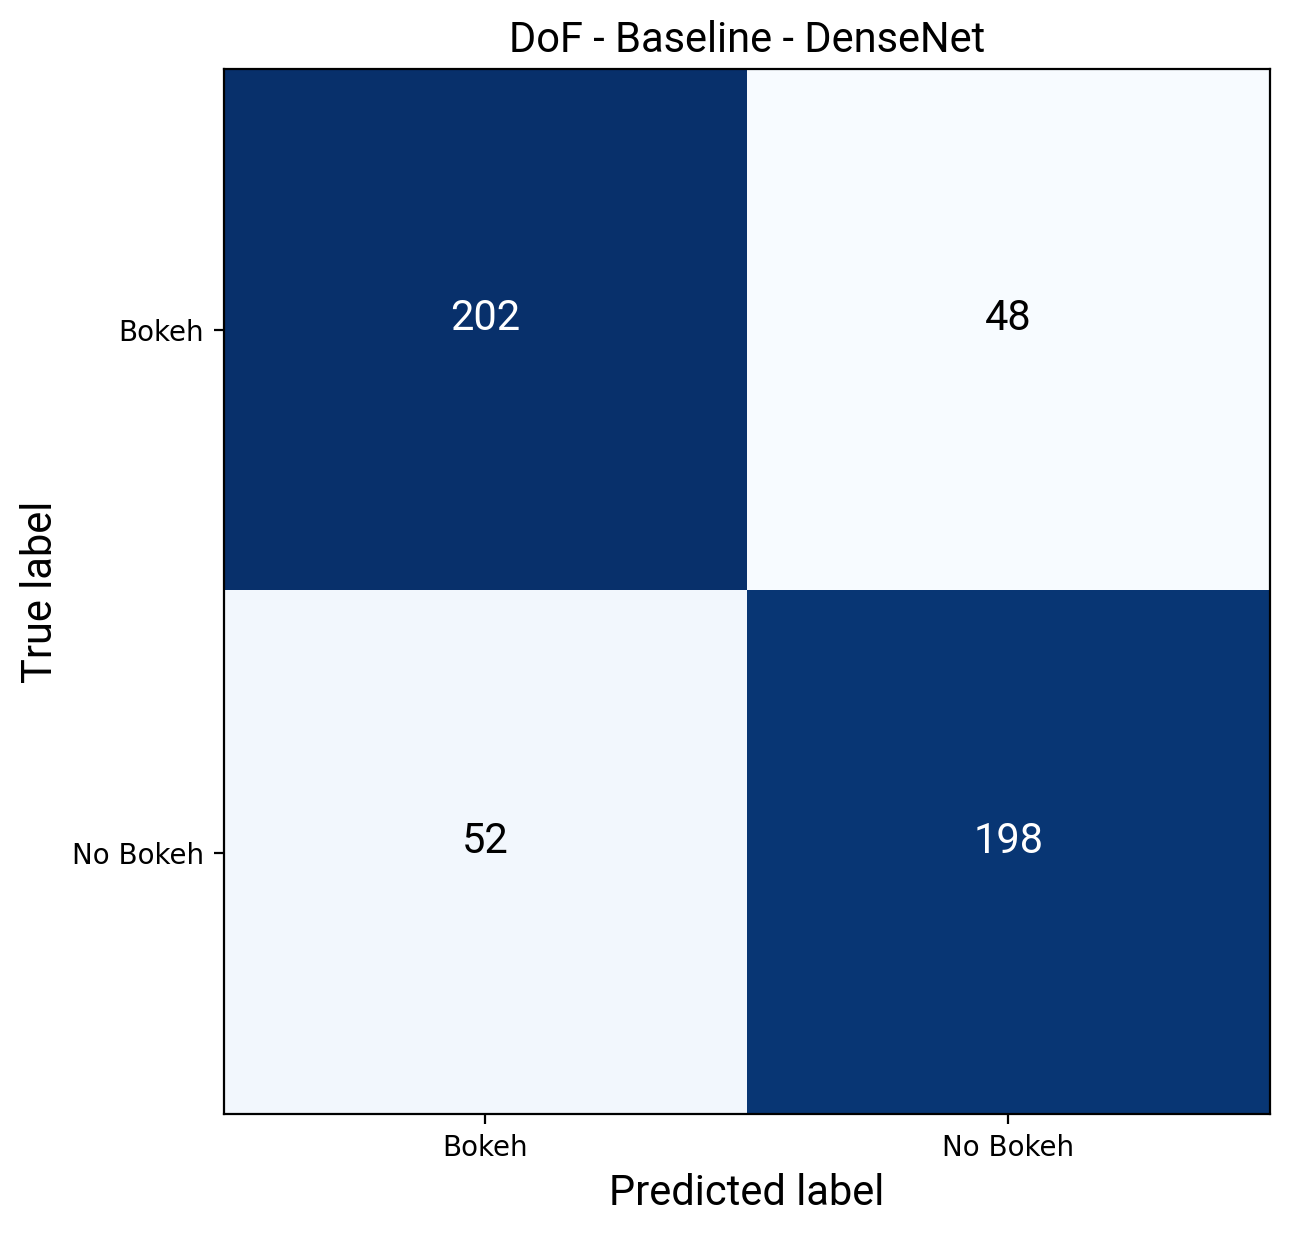
\includegraphics[width=.3\textwidth]{figures/chap5/dof/densenet/cm}}
    \subfigure{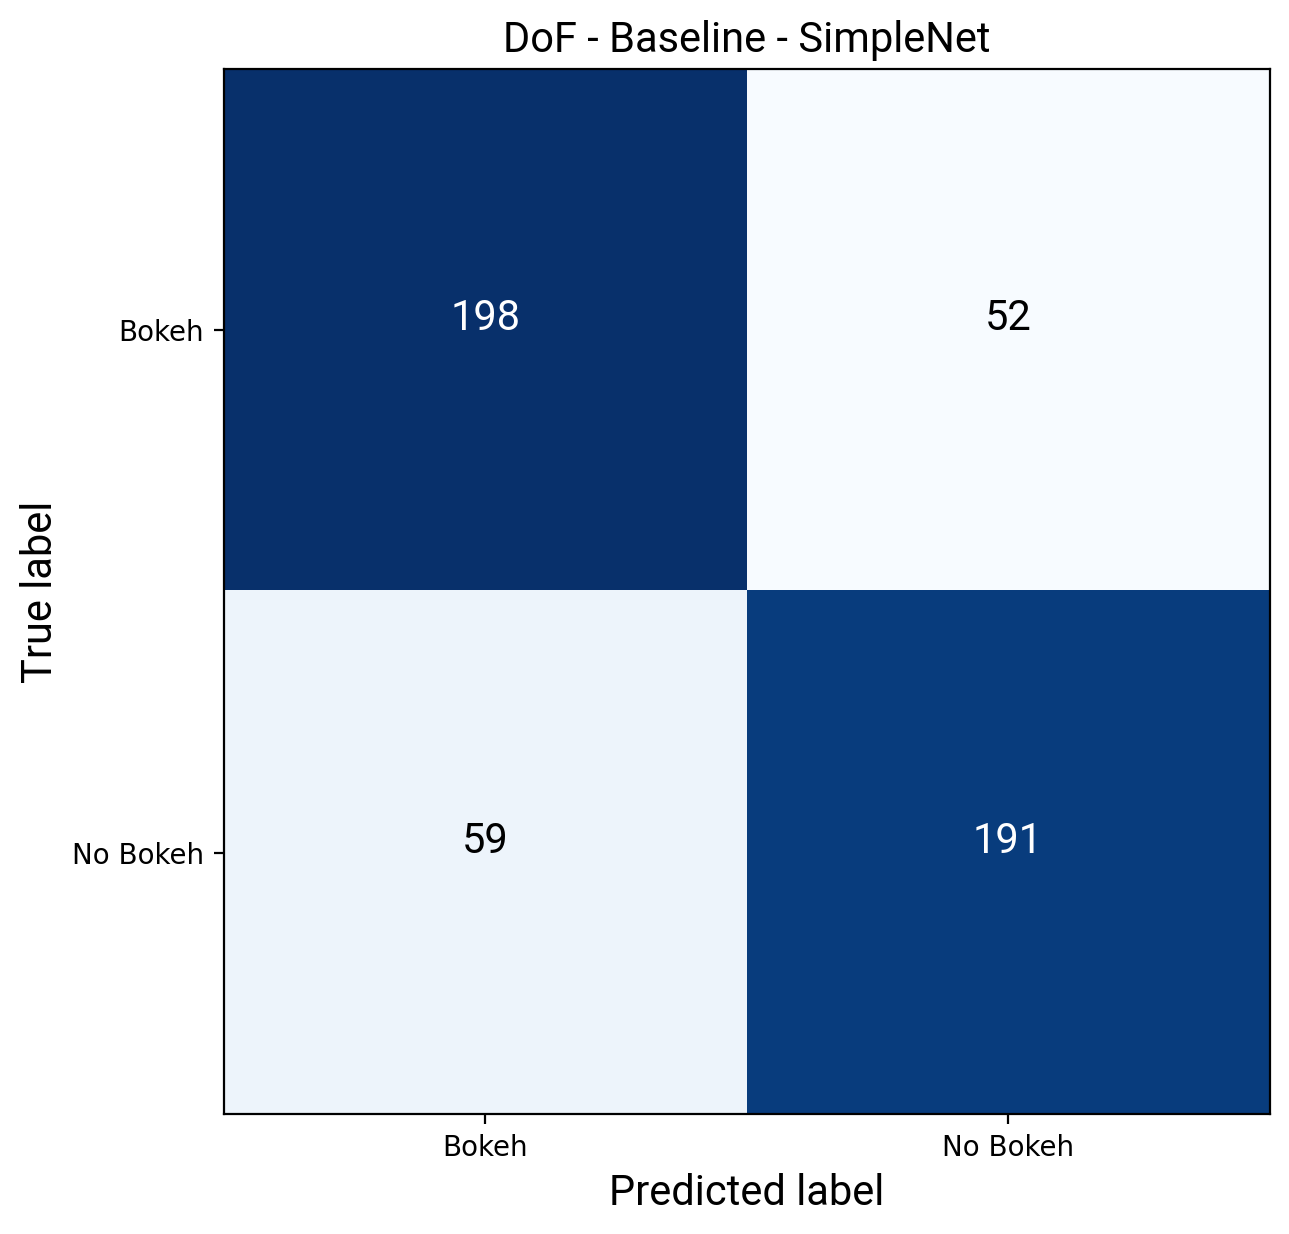
\includegraphics[width=.3\textwidth]{figures/chap5/dof/simplenet/cm}}
    \subfigure{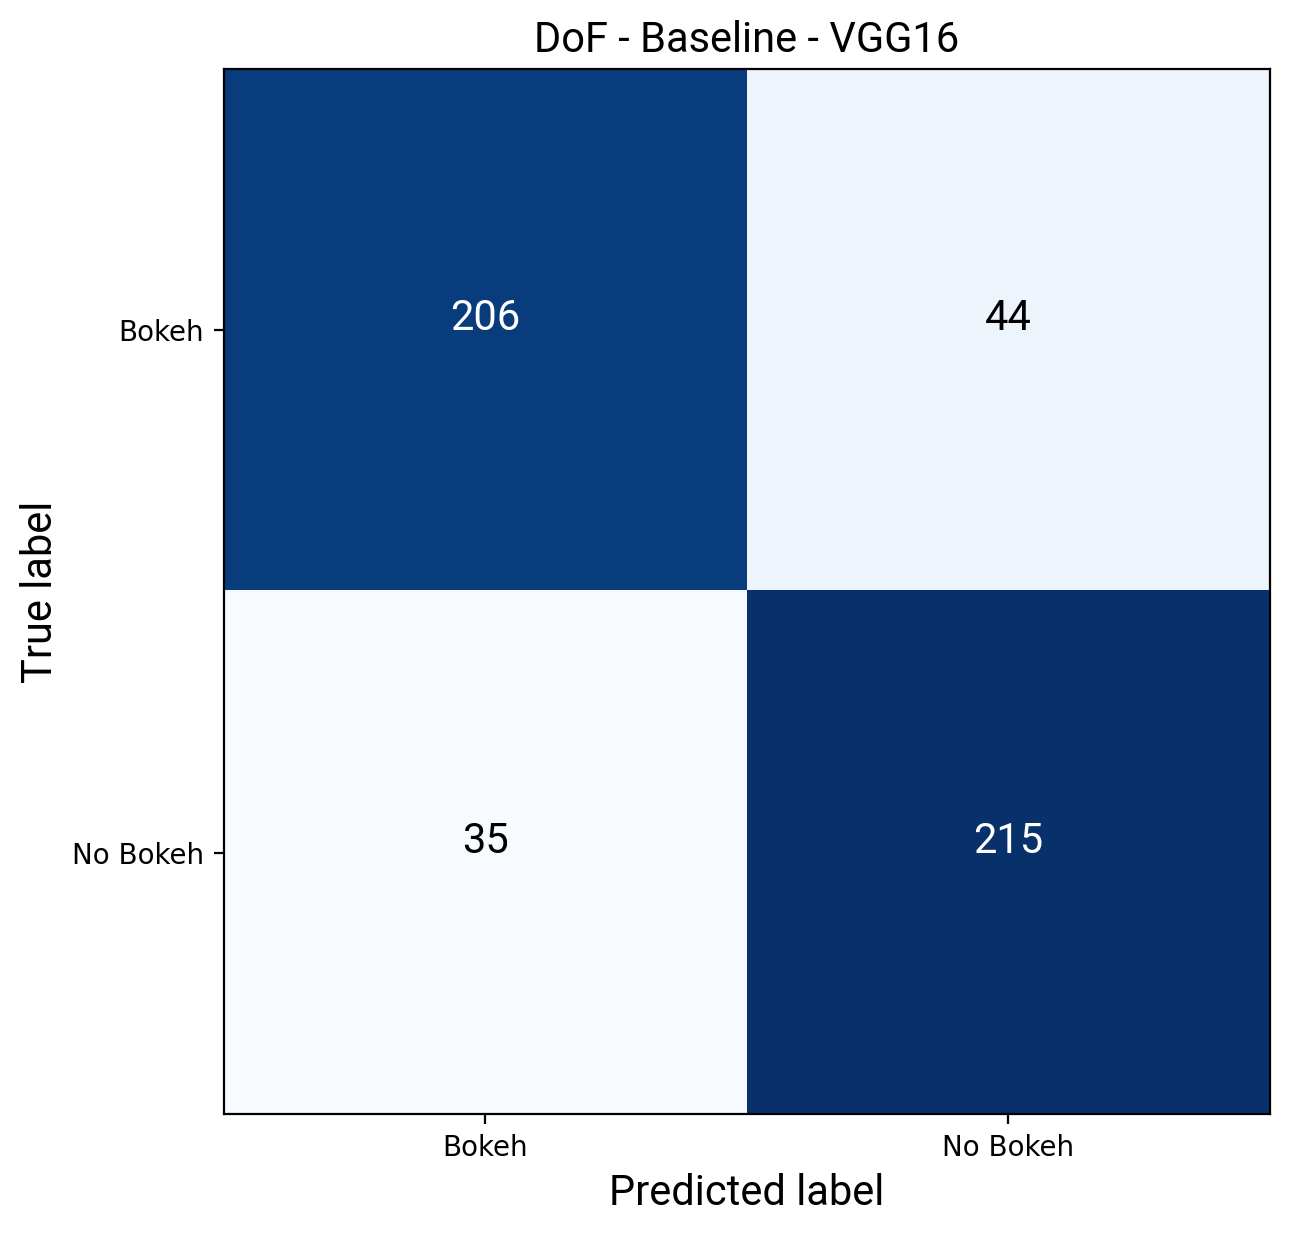
\includegraphics[width=.3\textwidth]{figures/chap5/dof/vgg/cm}}    
    \caption{Confusion matrix for the total of classifiers trained with DoF data set: (a) DenseNet, (b) SimpleNet, (c) VGG16}
    \label{c5:dof_cm}
\end{figure}

\subsection{Discussion}

Nevertheless the highest performed classifier, the classification problem between an image with bokeh and no bokeh seems that were successfully approached and tackled with a manually annotated dataset. With DoF data set we trained a classifier more effectively, though it was not a trivial task since most of previous works were based solely on EXIF metadata~\cite{guptaexif},~\cite{laurence2018camera}.

The performance of classifiers trained with DoF data set, outperforms the same architectures trained with almost 10$\times$ more data. In Figures~\ref{c5:dof_training_loss_history}-\ref{c5:dof_cm} we can observe that DenseNet model shows smoother fitting and validation loss curves. We observe something similar in VGG16 but with more overfitting, whereas fitting curve for validation set in SimpleNet is quite unstable.

Concerning confusion matrices, VGG16 records the less false negatives than others, whereas DenseNet has almost the same number of false positives as VGG16.

Motivated by the model's performance regarding a rather limited amount of annotated samples, given the annotation process is not trivial and essential photography perception is required, in the next section we present an active learning framework that aims to reduce the annotation effort in unlabelled samples and simultaneously maximize classification performance.
The active learning framework utilises i) the DoF data set as bootstrap set and ii) sets as an empirical baseline, the performance of the best report classifiers of this section.


\section{Active Learning - Experimental Outline}
\label{c5:active_learning}

In the previous sections, we presented a variety of trained classifiers on data sets with different labelling acquisition methodologies. The winner classifier achieved the highest performance and at the same time faster to train and more flexible were identified the \textbf{DenseNet} model based classifier trained on \textbf{DoF} data set.


Demonstrating the aforementioned strategies in Section~\ref{c5:section_passive_learning}, we will provide a complete deep active learning (DAL) methodology in the following sets of experiments divided into three categories as follows:
\begin{itemize}
 \item \textbf{Active learning indicator}, a method that will evaluate the feasibility of an active learning scenario with a selection strategy.
 \item \textbf{A/B test}, run an active learning experiment with variable number of labelled batches.
 \item \textbf{Simulating active learning}, evaluate the classification performance of two deep learning architectures in randomly and actively selected samples acquired from the same annotated data pool in variable number of batches and in incremental training.
\end{itemize}

\section{Active learning indicator}
\label{c5:section_active_learning_indicator}


When querying an active learner with unlabelled instances, we ask which samples are going to get annotated next. Those samples are selected based on i) an active learning query setting %pool based
and ii) a query strategy method. %uncertainty sampling

Before applying an active learning strategy, we should assess the ``passive'' learned classifier to fulfill certain guarantees. 
\begin{enumerate}
 \item a classifier with relative competent baseline performance will play the role of an active learner.
 \item an evaluative measurement that will show the classifier's ability to identify the informativeness in potentially labelled samples, that eventually have the higher performance impact when they get included to the training set rather than select them randomly.
\end{enumerate}


Before formulating an active learning algorithm, we will conduct a procedure to measure the classifier's ability to identify the most informative and potentially labelled samples in order to determine an active learning strategy.

So far, in Section~\ref{c5:dof_results} we developed a DenseNet based model, trained on 560/140 images used for training and validation and achieved 80\% accuracy on DoF dataset, using random sampling - requiring a photography expertise to obtain the labels.

In this section, we conduct a procedure that utilises the trained densenet model as an active learner $\mathbb{C}$, to produce the posterior probabilities from the softmax output on the pool$\mathbb{U}$ containing 12312 unlabelled samples with horizontal images. Next, we create pool$\mathbb{L}_{rnd}$, by randomly selecting and annotating 1000 balanced samples, from the unlabelled pool$\mathbb{U}$ and perform the same procedure.

%We should note that there is no overlapping between randomly and actively selected samples.

The calculated posteriors were sorted and mapped into five posterior probability bins, as shown in Table~\ref{c5:probability_bins}.
\begin{table}[ht!]
    \centering
    \footnotesize
    \begin{tabular}{|l|c|}
    \hline
    \textbf{Bins} & Posterior probability range \\ \hline
    Bin1 & $<$60\%) \\ \hline
    Bin2 & [60\%-70\%) \\ \hline
    Bin3 & [70\%-80\%) \\ \hline
    Bin4 & [80\%-90\%) \\ \hline
    Bin5 & [90\%-100\%]  \\ \hline
    \end{tabular}
    \caption{Posterior probability bins for each corresponded prediction probability range}
    \label{c5:probability_bins}
\end{table}

The cardinality of calculated probabilities from pool$\mathbb{U}$ and pool$\mathbb{L}_{rnd}$ are illustrated in Figures~\ref{c5:fig_unlabelled_inference},~\ref{c5:fig_random_cardinality_bins}.
We can observe that both figures follow the same distribution, a good sign that randomly picked samples are independent and identical distributed(i.i.d).

\begin{figure}[ht!]
    \centering  
    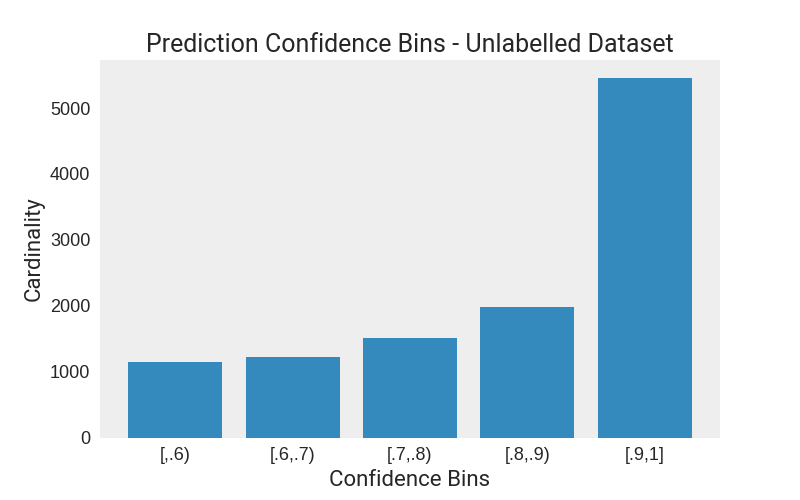
\includegraphics[width=.5\textwidth]{figures/chap5/al/indicators/cardinality/pred_conf_unseen_dataset}
    \caption{Cardinality of calculated posterior probabilities clustered in 5 probability bins for 12312 unlabelled samples.}
    \label{c5:fig_unlabelled_inference}
\end{figure}


\begin{figure}[ht!]
    \centering  
    %\subfigure[]{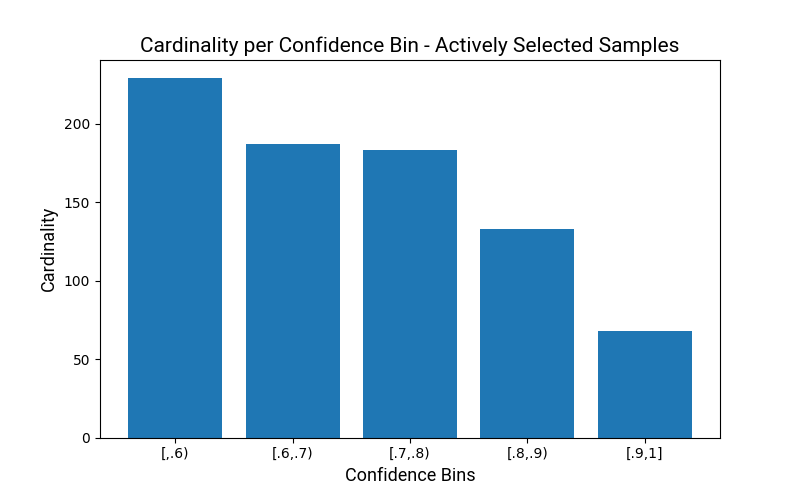
\includegraphics[width=.45\textwidth]{figures/chap5/al/indicators/cardinality/pred_conf_cardinality_active}}
    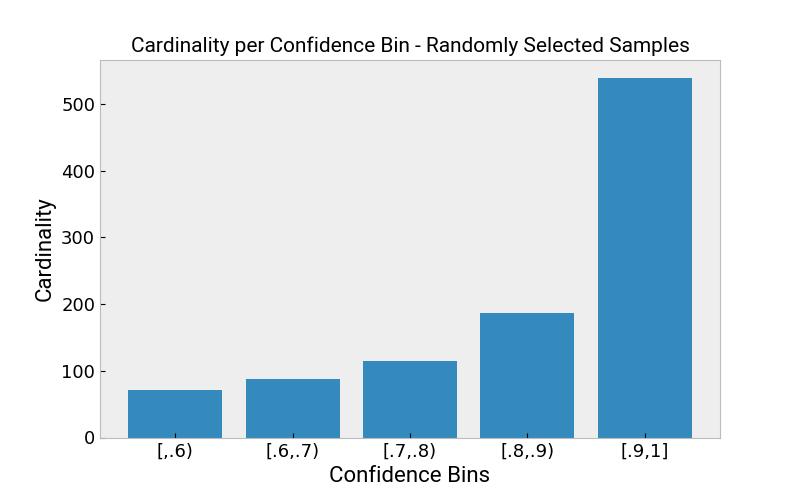
\includegraphics[width=.45\textwidth]{figures/chap5/al/indicators/cardinality/pred_conf_cardinality_random_1000}
    \caption{Cardinality of calculated posterior probabilities clustered in 5 bins for 1000 randomly selected samples.}
    \label{c5:fig_random_cardinality_bins}
\end{figure}

To measure the informativeness measure, from the annotated pool$\mathbb{L}_{rnd}$ we calculated the accuracy and true positive rate(TPR), for each confidence bin. Figures~\ref{c5:random_indicator_bins_accuracy},~\ref{c5:random_indicator_bins_tpr} illustrate the results for accuracy and TPR accordingly.

\begin{figure}[ht!]
    \centering  
    %\subfigure[]{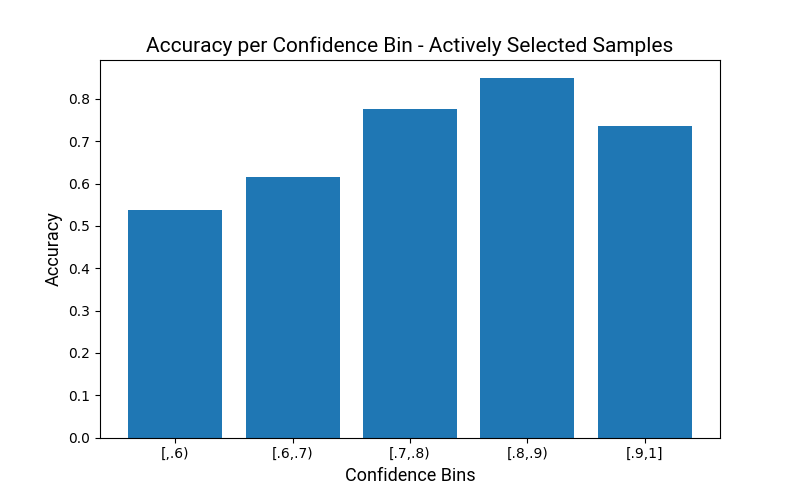
\includegraphics[width=.45\textwidth]{figures/chap5/al/indicators/acc/pred_conf_acc_active}}
    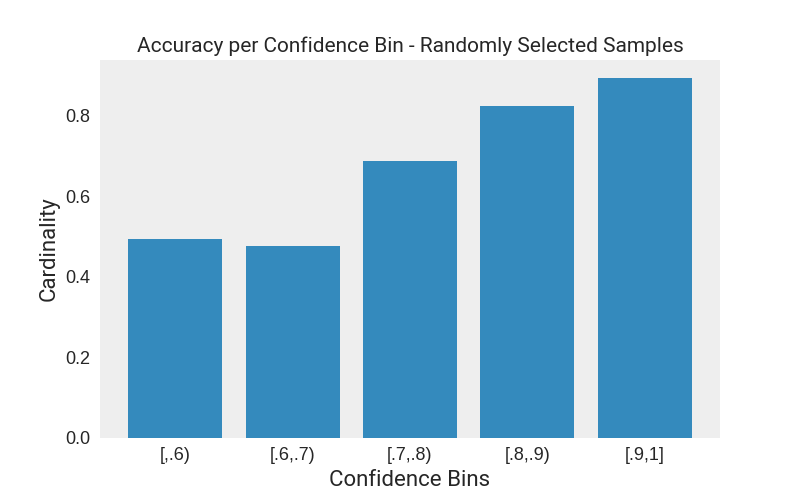
\includegraphics[width=.45\textwidth]{figures/chap5/al/indicators/acc/pred_conf_acc_random_1000}
    \caption{Measured accuracy for each posterior probability confidence bin for 1000 randomly selected samples.}
    \label{c5:random_indicator_bins_accuracy}
\end{figure}

\begin{figure}[ht!]
    \centering  
    %\subfigure[]{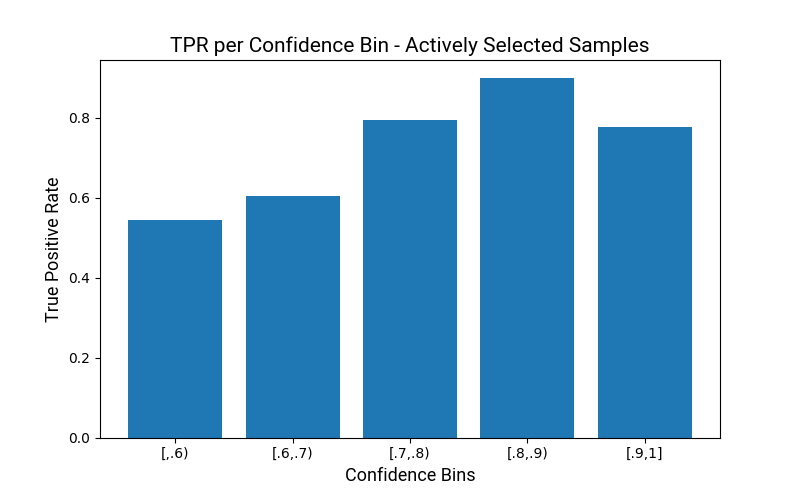
\includegraphics[width=.45\textwidth]{figures/chap5/al/indicators/tpr/pred_conf_tpr_active}}
    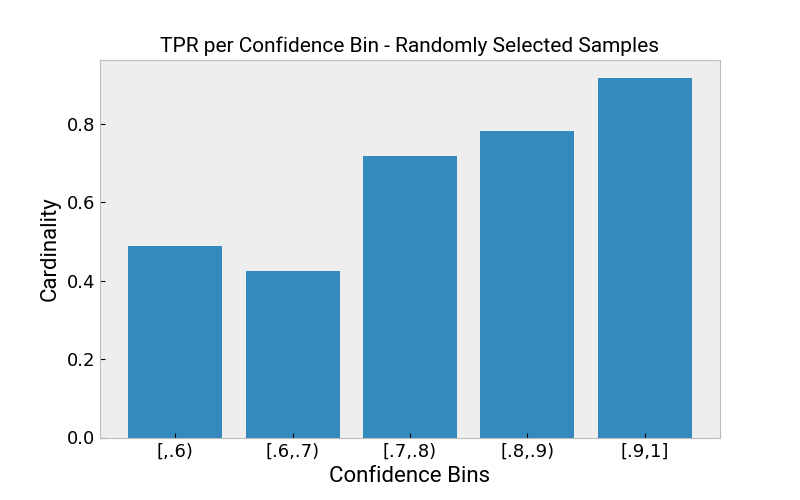
\includegraphics[width=.45\textwidth]{figures/chap5/al/indicators/tpr/pred_conf_tpr_random_1000}
    \caption{Measure True Positive Rate(TPR) for each posterior probability confidence bin in 1000 randomly selected samples.}
    \label{c5:random_indicator_bins_tpr}
\end{figure}

Algorithm~\ref{c5:al_indicator_algorithm} describes the aforementioned process.

\begin{algorithm}
\caption{Active Learning Indicator}
\label{c5:al_indicator_algorithm}
\begin{algorithmic}[1]
\Procedure {Informativeness Measurement}{}
    \State Create a pool$\mathbb{U}$ of unlabelled samples
    \State Randomly select i.i.d samples and create a data set in pool$\mathbb{L}_{rnd}$
    \State Query pool$\mathbb{L}_{rnd}$ on active learner $\mathbb{C}$
    \State Obtain posterior probabilities with softmax
    \State Cluster posterior probabilities in 5 probability bins [,.6), [.6,.7), [.7,.8), [.8,.9), [.9,.1]
    \State Obtain labels for pool$\mathbb{L}_{rnd}$
    \State Measure accuracy and TPR for each probability bin
\EndProcedure
\end{algorithmic}
\end{algorithm}



Studying figures~\ref{c5:random_indicator_bins_accuracy},~\ref{c5:random_indicator_bins_tpr} we reach to the following conclusion concerning informativeness measurement on the annotated randomly selected pool. It is clear that accuracy and TPR shows and incremental performance as the confidence of the classifier increases.
More specifically Bin1 is 49\% accurate while Bin5 achieves 89.4\% accuracy. Concerning TPR, is measured in the same neighborhood.

For the most uncertain unlabelled samples, although their number is smaller than of high confident, it is reasonable to ask for queries from the active learner, send them for annotation and return them to the training set, as they can contribute to a greater impact on the classifier improving the decision boundary.

The measurements above can justify classifier's discrimination ability to correctly classify an unknown pool from the same distribution, where high-confidence unlabelled instances score a posterior probability above $\sim 90\%$, meaning that these instances are close to the learned samples in the CNN's feature space.

Thus, pseudo labelling high confident inferences will induce a 10\% of error in training set, is a reasonable data augmentation in weakly-supervised fashion following a CEAL~\cite{wang2016cost} practice.

The DenseNet based classifier trained on DoF dataset, shows that can be used as an active learner to bootstrap an active learning setting as it is capable to correctly classify high confident samples while the low confident ones are misclassified, based on the groundtruth.
We can safely assume, that choosing samples in an active selection fashion, by annotating the most uncertain ones is highly possible to achieve higher performance rates with less annotation budget.

In the next section we perform an A/B test using the baseline classifier as an active learner and DoF data set as a bootstrap set to initiate the process.

\newpage
\section{A/B test}
\label{c5:section_ab_test}

In this section, we conduct an A/B test, demonstrating the use of an deep active learning setting along with a regular passive learner.
Our objective is to apply an active learning framework applying uncertainty sapling(US), simultaneously with a passive learning approach, evaluating both methods. The motivation is to answer to question if a data-driven selection sample approach can improve the classification performance with less annotated data over a random/regular selection with passive learning.
Thus we form a hypothesis in order to observe the potential differences between the two approaches.

The A/B experiment is formed as follows:
\begin{itemize}
 \item Use DoF data set as bootstrap set and baseline classifier as active learner to initiate the process.
 \item Collect a randomly selected data set as regular and obtain labels from a human annotator.
 \item Select active learning pool based setting and uncertainty sampling approach combined with a cost effective selection scheme strategy(pseudolabelling).
 \item Perform a single active learning round, send the instances that active learner indicated as less confident/more informative and obtain labels from a human annotator.
 \item Create training pools with random-\textbf{PoolA} and actively selected-\textbf{PoolB} samples.
 \item Perform two individual experiments for PoolA \& PoolB, in distinct training rounds, using a varying number of batched instances transferred from the pool to DoF training/validation sets without updating the model's weights and bias, train from scratch re-assess the experiment on DoF testing set.
 \item Plot learning curves of measured accuracies for every learning step.
\end{itemize}

To begin with, we will use the baseline densenet model as the active learner $\mathbb{C}$ once. The DoF training/validation set will be used as bootstrap set to initiate the process and DoF testing set with the identical 500 test samples as in Section~\ref{c5:section_passive_learning} to evaluate the model in each training round.

The notion behind the creation of data pools is to evaluate randomly and actively selected sets using uncertainty sampling and cost effective labelling(pseudolabel) strategies. 
Concerning cost effective annotation methodology, in order to not violate the statistical properties of the experiment, a certain number of high confident instances will used in both pools and will be identical using different groundtruth(real and pseudolabelled).

\subsection{Random Selection - Pool A}

To obtain a randomly selected pool we utilized pool $\mathbb{X}^U_{random} \subseteq  \mathbb{X}^U$ - $\mathbb{X}^L_{bootstrap}$, the same as generated in Section~\ref{c5:section_active_learning_indicator}.

The majority of samples, almost half of them are belong to the most confident cluster \textit{bin5}, whereas the rest are distributed to the other clusters.
Using $\delta=[90\%,100\%)$, we selected $k=200$ samples from \textit{bin5} named after \textbf{RA1} and obtained labels. Same samples will be used with pseudolabels for active selected pool. The rest 800 samples were annotated and named after \textbf{RS1}, $ RS1 \cup  RA1 = \mathbb{X}^L_{random}$.

To form a balanced pool set, we undersampled RS1 from the majority class and generated a pool consisted of 720 samples named after \textit{RS1-b}, which contains samples for all confidence bins. Finally RA1 which contain only high confident samples, is merged on top of RS1-b creating \textit{PoolA}, as depicted in Figure~\ref{c5:figure_ab_pool_a}. Algorithm~\ref{c5:algorithm_ab_poola} describes the process of randomly selected PoolA generation. PoolA data set is formulated as follows: 

\begin{ceqn}
\begin{align}
  \text{RA1} \subseteq \mathbb{X}^L_{random}, \text{RA1} \neq \text{RS1} , \text{RS1-b} \subseteq \text{RS1}
\end{align} 
\begin{align}
    \text{PoolA} =  \text{RS1-b} \cup \text{RA1}
\end{align} 
\begin{align}
   \text{PoolA} \subseteq  \mathbb{X}^L_{random}
\end{align} 
\label{c5:random_pool_a}
\end{ceqn}

\begin{figure}[ht!]
    \centering  
    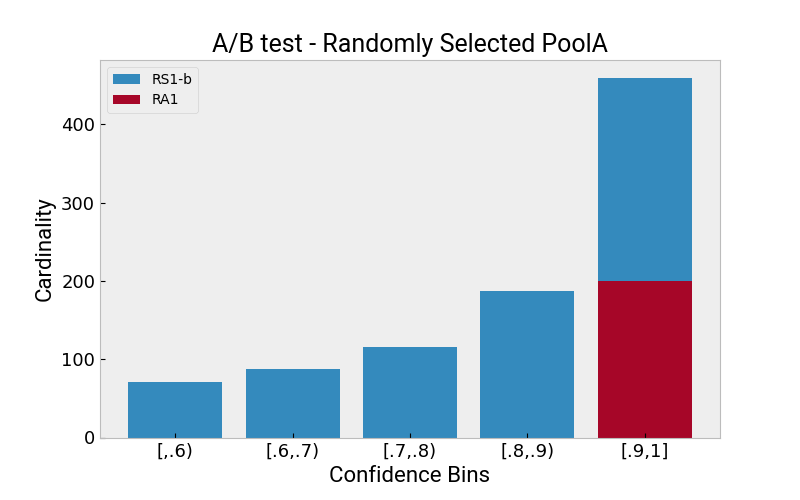
\includegraphics[width=.65\textwidth]{figures/chap5/ab_test/dataset/pred_conf_random}
    \caption{Randomly selected PoolA structure and distribution of posterior probabilities clustered in 5 bins for 720+200 randomly selected and balanced samples.}
    \label{c5:figure_ab_pool_a}
\end{figure}


\begin{algorithm}
\caption{Random PoolA}
\label{c5:algorithm_ab_poola}
\begin{algorithmic}[1]
\Require active learner C, Random selection $X_{rnd}$, pseudolabel confidence threshold $\delta$
\Procedure {Create random PoolA}{}
    \State Obtain labels for $X_{rnd}$
    \State Query $X_{rnd}$ $\rightarrow$ C
    \State Cluster $X_{rnd}$ posteriors and apply $\delta$
    \State Holdout and create a high confident batch $RA1$
    \State $PoolA$ = $X_{rnd}$ + $RA1$
\EndProcedure
\end{algorithmic}
\end{algorithm}



\subsection{Active Selection - Pool B}
\label{c5:section_active_poolb}
%13518
The rest of total 11318 unlabelled samples $\mathbb{X}^U_a$, leaving out
\textit{bootstrap} $\mathbb{X}^L_{bootstrap}$ and $\mathbb{X}^L_{PoolA}$,
are defined as $\mathbb{X}^U_a$ = $\mathbb{X^U}$ - $\mathbb{X}^L_{bootstrap}$ - $\mathbb{X}^L_{PoolA}$.

$\mathbb{X}^U_a$ is queried to the active learner to compute the prediction uncertainty given an informativeness score $s_i \in [0.5,1]$ for every sample. Informativeness is computed using the cross-entropy of softmax predictions keeping the dominant prediction. Scored instances are ranked in ascending order based on their computed uncertainty and are clustered in five prediction probability bins.

Clustered instances are prefiltered on the most uncertain by selecting $\delta k \leq K$ where $\delta= [50\%,60\%)$ probabilities, $k$ the selected instances in $\delta$ and $K$ all uncertainty measured instances.
Thus \textit{bin1}$=\delta k$, is send to human oracle to obtain their labels using membership query synthesis.

More specifically we have actively selected and annotated a pool of 720 equally balanced samples from \textit{bin1}, and named after \textbf{AS1}, containing the most uncertain predicted samples, ranked in ascending order.

\textbf{RA1} pool will be utilized with pseudolabels obtained from query stage using the dominant prediction and pass it to an argmax as Eq 5.7 denotes.

\begin{ceqn}
\begin{align}
    \hat{y} = \text{argmax}_y P(\hat{y}|x;\theta)
\end{align} 
\label{c5:eq_argmax}
\end{ceqn}

Finally the pseudolabelled \textbf{RA1} pool named after \textbf{RA1-aug} is merged on top of \textbf{AS1} creating \textit{PoolB}. Algorithm~\ref{c5:algorithm_ab_poolb} describes the process we followed to generate actively selected PoolB.
\textit{PoolB} as depicted in Figure~\ref{c5:figure_ab_pool_b} and is formulated as follows: 

\begin{ceqn}
\begin{align}
      \text{RA1-aug} \approx \text{RA1}, \text{AS1} \subseteq \mathbb{X}^U_a
\end{align} 
\begin{align}
       \text{PoolB} = \text{RA1-aug} \cup \text{AS1}
\end{align} 

\label{c5:active_pool_b}
\end{ceqn}

\begin{figure}[ht!]
    \centering  
    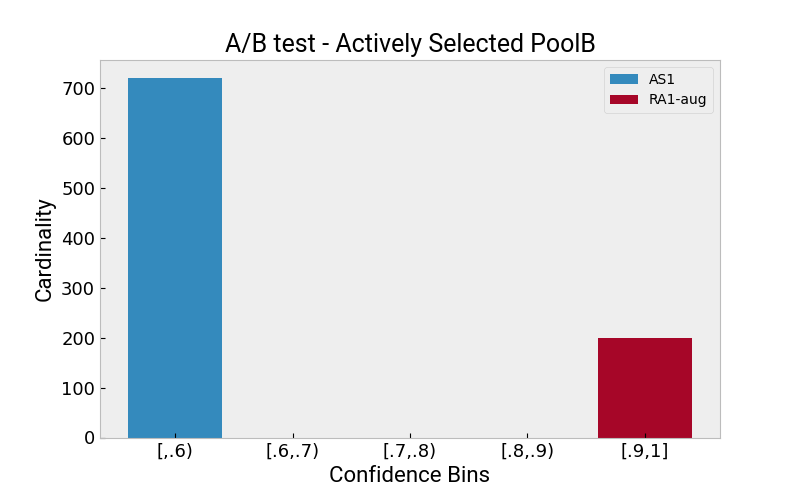
\includegraphics[width=.65\textwidth]{figures/chap5/ab_test/dataset/pred_conf_active}
    \caption{Actively selected PoolB structure and distribution of posterior probabilities clustered in 5 bins for 720 actively selected and balanced samples + 200 high confident pseudolabelled samples.}
    \label{c5:figure_ab_pool_b}
\end{figure} 

\begin{algorithm}
\caption{Active PoolB}
\label{c5:algorithm_ab_poolb}
\begin{algorithmic}[1]
\Require active learner C, $X_{U}$, $RA1$
\Procedure {Create active selected PoolB}{}
    \State Query unlabelled set $X_{U}$ $\rightarrow$ C
    \State Cluster $X_{U}$ posteriors
    \State Obtain labels for the lowest probability cluster
    \State Rank labelled samples in ascending order by probability $\rightarrow$ $RS1$
    \State Pseudolabel $RA1$ using the predicted class inferred from queries, as groundtruth  $\rightarrow$ $RA1-aug$
    \State $poolB$ = $RS1$ + $RA1-aug$(ranked)
\EndProcedure
\end{algorithmic}
\end{algorithm}


\subsection{Experimental setup}

To initiate the process we used the training/validation DoF dataset, similarly to Section~\ref{c5:dof_results}, to create the active learner.

In Section~\ref{c5:section_batch_mode_learning}, we elaborate on the batch-mode learning where for every learning cycle, data is systematically added in chunks back to the bootstrap set. Eventually when a learning cycle completes a new classifier is trained.

In each training cycle for both randomly/actively selected samples, the classifier is evaluated on the test set of DoF data set comprised of 500 samples. The test set is not queried or augmented and is kept intact.
 
Performance results are drawn in learning curves, for every individual number of annotated instances picked from random/active pool.

For both experiments random and active, we applied a varying sequential selection from 100-920 samples per learning round. Every selection round is increased by 100 samples except from the last one which adds 120. The selected samples are added to the bootstrap(DoF) set in training/validation splits by 80/20 ratio.
Each learning round picks the next batch from the ranked pool and adds to the DoF set, always including the previously picked batches. Thus a new classifier is produced and evaluated in total of 9 learning rounds until the data pool is depleted.

Concerning random selection, samples are selected randomly from \textit{PoolA}.
In active selection, the active learner is queried only once on \textit{PoolB}, before the experimental process starts, to rank the actively selected pool, as described in Section~\ref{c5:section_active_poolb}.
For each learning cycle, new samples are obtained directly from the pool and neither the active learner is updated from a new one or human annotator intervenes in the process.
The samples are picked based their uncertainty score in ascending probability order from the most to the less uncertain prediction.

We measure the classification accuracy and report the mean values for 3 runs with 3 different random seeds. Throughout the experiments, we use the same hyperparameters as the baseline model, since active learner is not updated.

\begin{algorithm}
\caption{Pseudo-algorithm of A/B training process.}
\label{c5:algorithm_ab_training}
\begin{algorithmic}[1]
\Require DoF bootstrap set $X$, active learner $C$, $Pool_{A}$, $Pool_{B}$, batch-size $k$, random seed[0,10,100] $seeds_{rnd}$
\Procedure {A/B training process}{}
    \State batch-size=100, samples that will be picked next
    \For{pool in [$Pool_{A}$, $Pool_{B}$]}
        \For{rs in $seeds_{rnd}$}
            \State apply rs
            \Repeat
                \State Pick the k from pool and append it to $X$, $X_{new}$ = $X$ + k
                \State Train classifier on new $X_{new}$ until convergence
                \State Evaluate on DoF test set
            \Until{pool is depleted}
        \EndFor
    \EndFor
\EndProcedure
\end{algorithmic}
\end{algorithm}


\subsection{Results - Discussion}

Figure~\ref{c5:figure_ab_test_results} shows Accuracy, F1 and Loss for two different experiments using the same deep learning classifier. We have evaluated the performance of randomly and actively selected data pools, on the DoF testing set, using pool-based active learning strategy and selecting the next batch based on uncertainty sampling. 
Moreover the last two batches, concerning 800 and 920 samples drawn from \textit{PoolB} include the most confident queries that were pseudolabelled using the dominant predicted class as groundtruth.

\begin{figure}[ht!]
    \centering  
    \subfigure[]{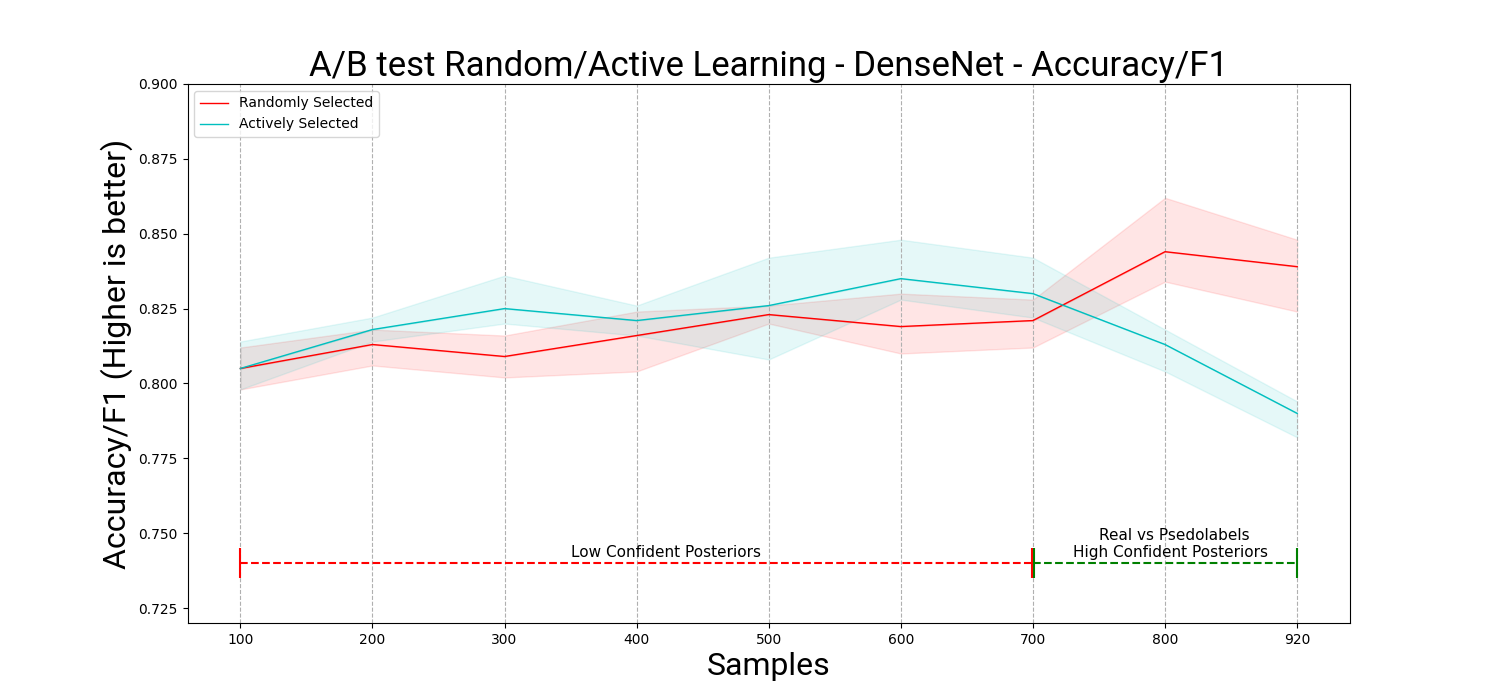
\includegraphics[width=.75\textwidth]{figures/chap5/ab_test/accuracy_f1}}
    \subfigure[]{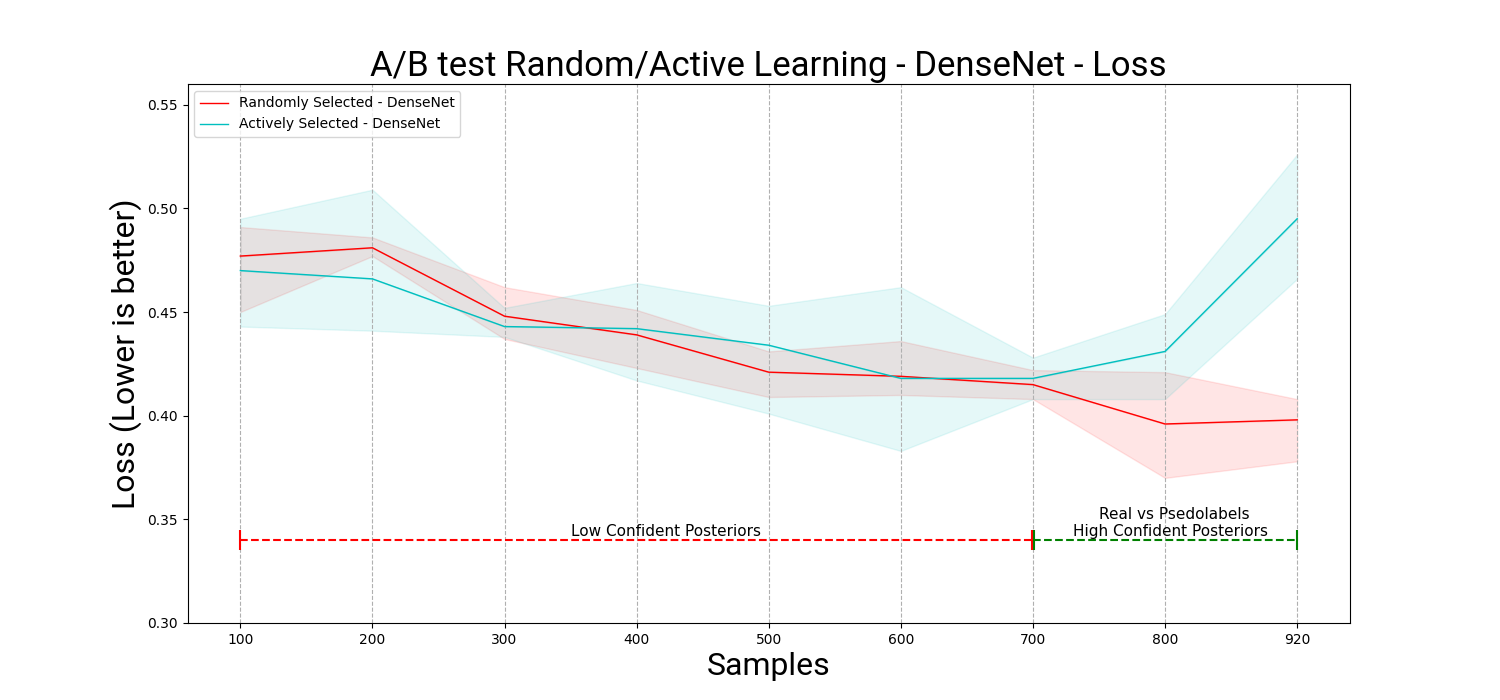
\includegraphics[width=.75\textwidth]{figures/chap5/ab_test/loss}}
    \caption{Experimental results for measured (a) Accuracy/F1-macro, (b) Loss in A/B test. Each chart is the mean of 3 runs with different random seeds, with the deviation of maximum and minimum measured values.}
    \label{c5:figure_ab_test_results}
\end{figure}

\begin{figure}[ht!]
    \centering  
    \subfigure[]{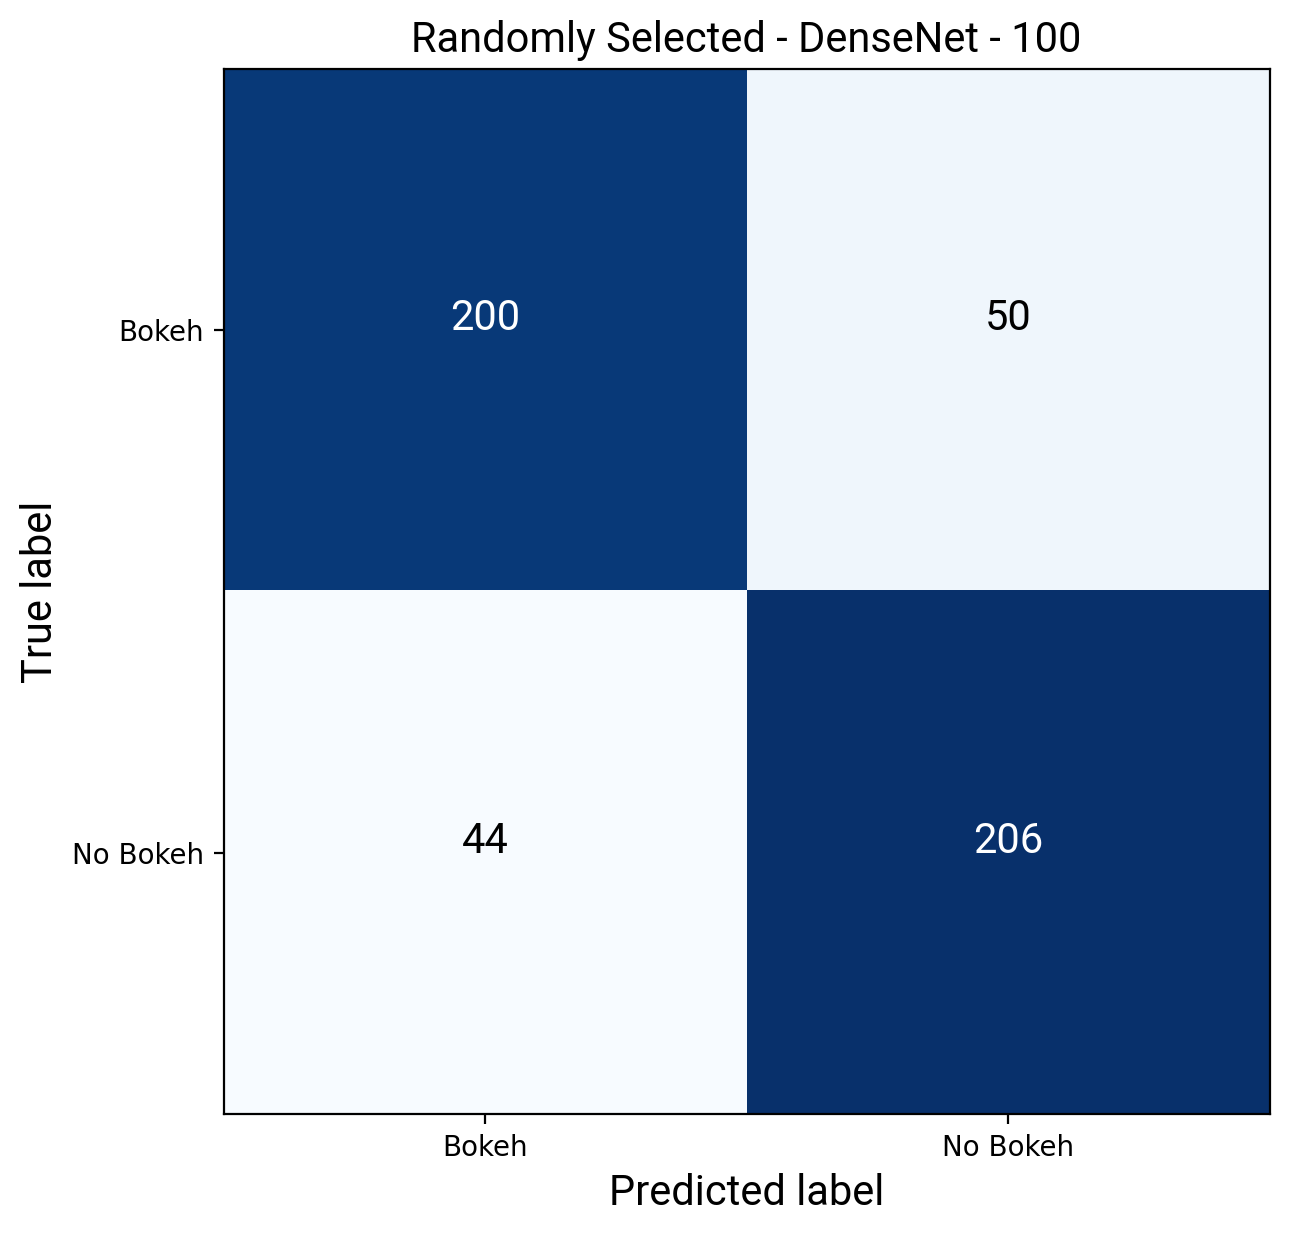
\includegraphics[width=.3\textwidth]{figures/chap5/ab_test/random-densenet-100_cm}}
    \subfigure[]{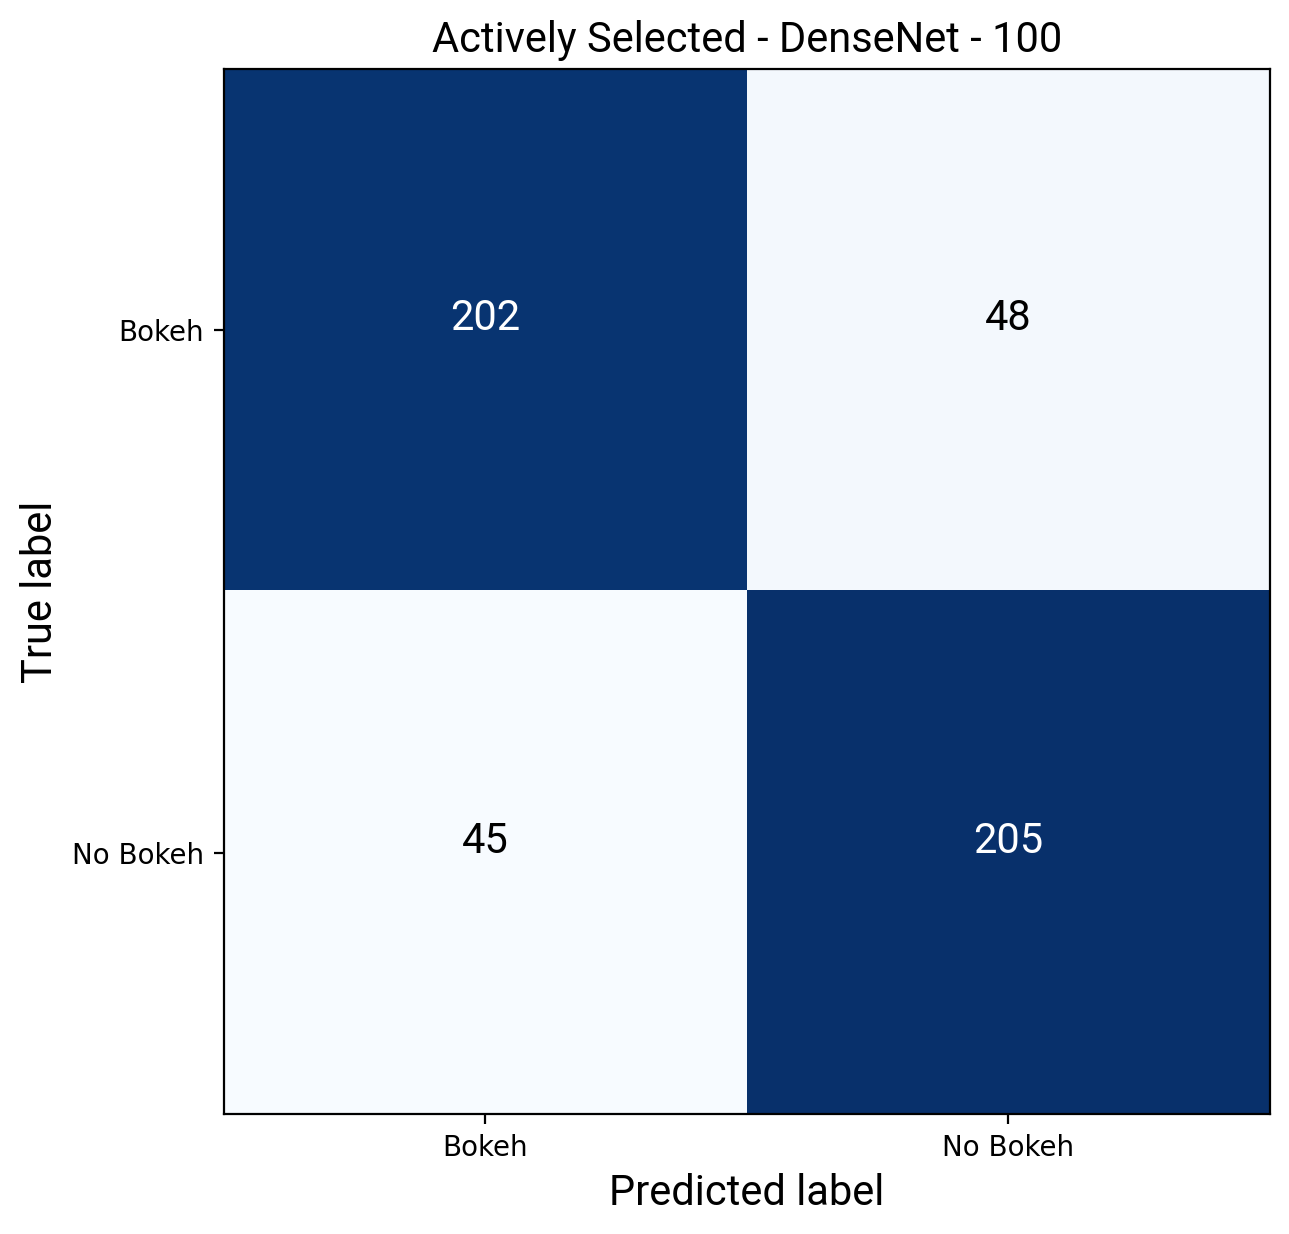
\includegraphics[width=.3\textwidth]{figures/chap5/ab_test/active-densenet-100_cm}}
    \caption{Confusion matrices of the best recorded run for 100 extra annotated samples in A/B test: (a) random, (b) active}
    \label{c5:figure_cm_100}
\end{figure}

\begin{figure}[ht!]
    \centering  
    \subfigure[]{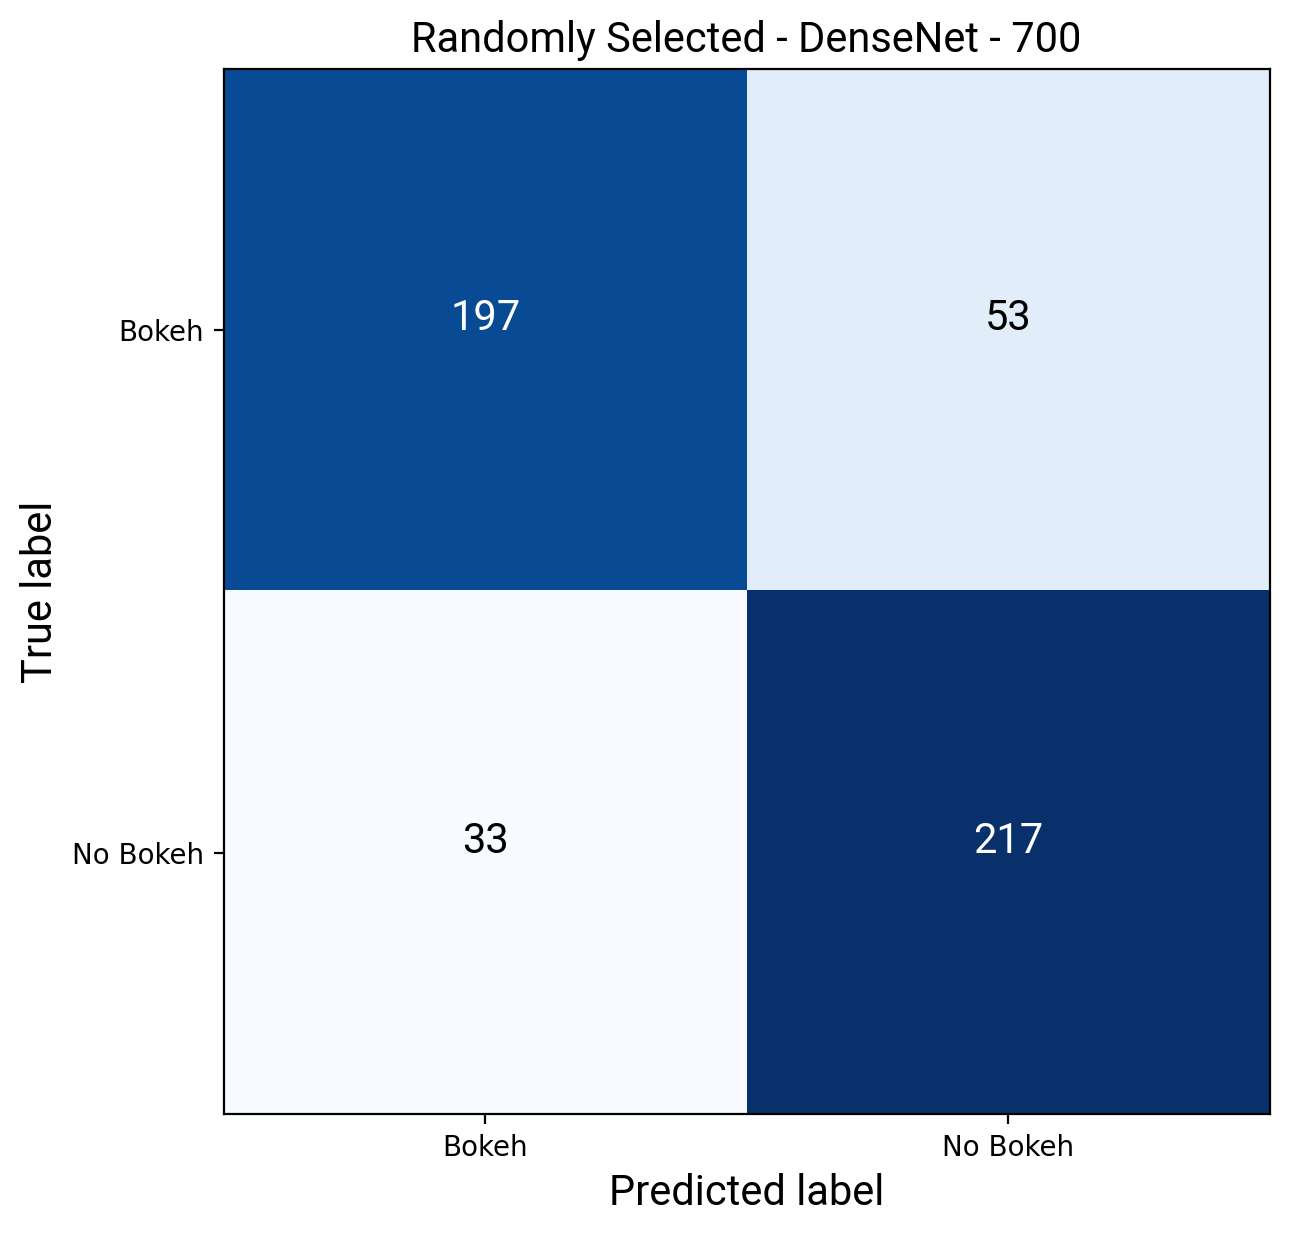
\includegraphics[width=.3\textwidth]{figures/chap5/ab_test/random-densenet-700_cm}}
    \subfigure[]{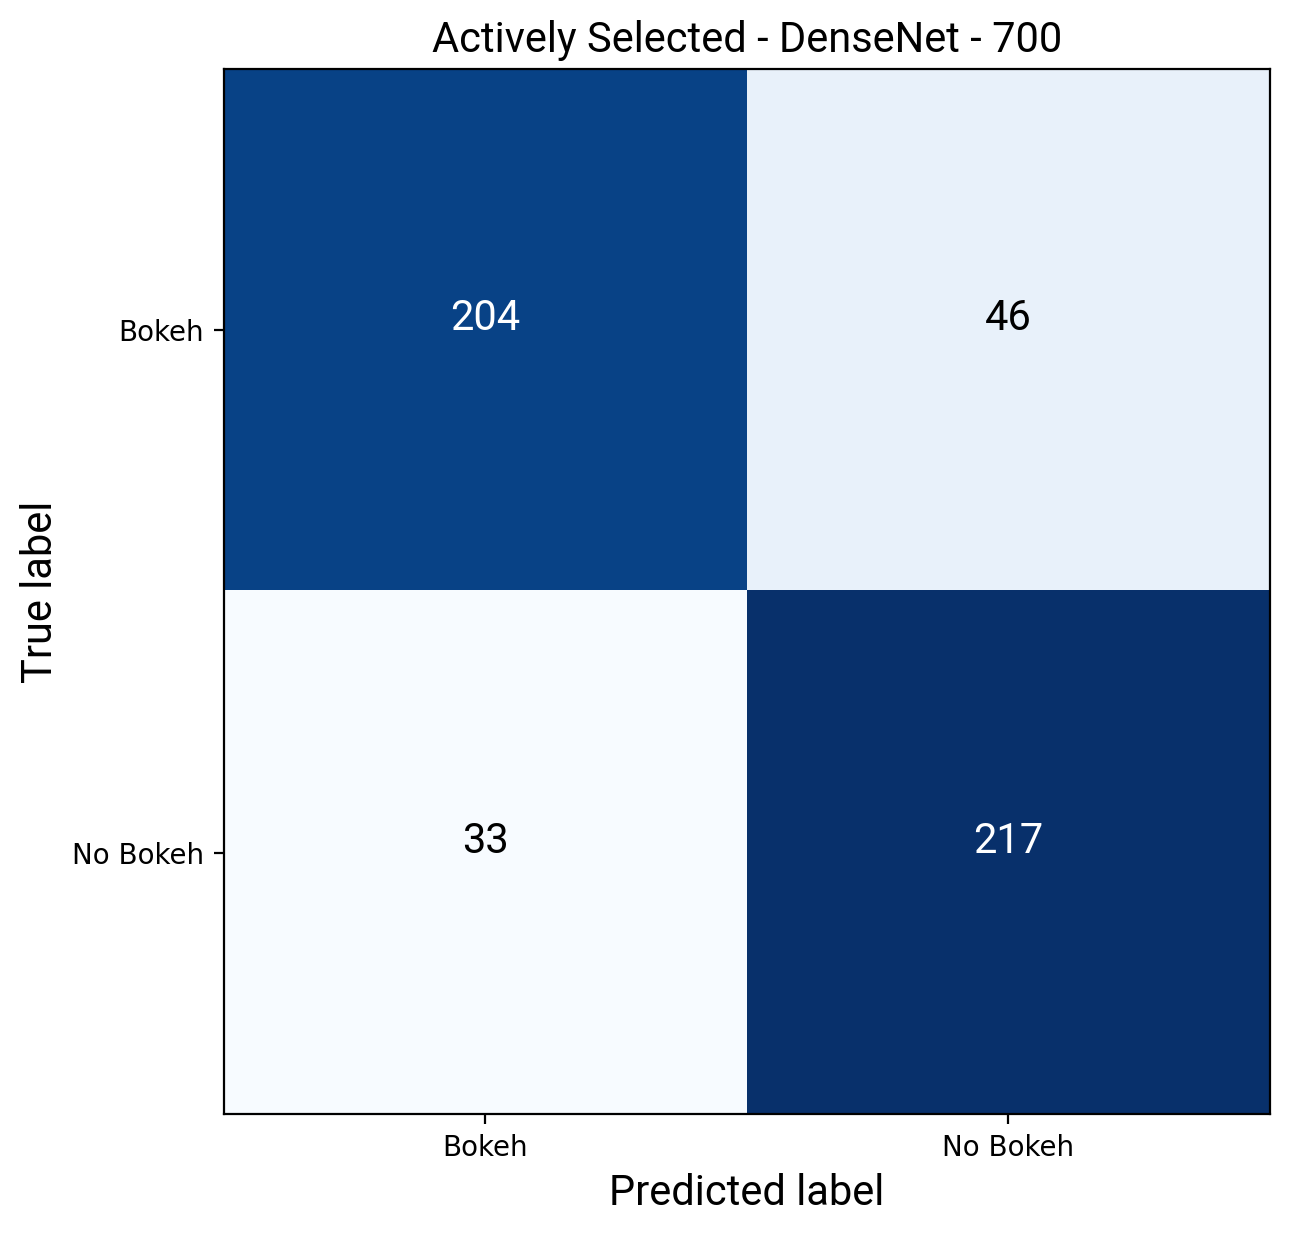
\includegraphics[width=.3\textwidth]{figures/chap5/ab_test/active-densenet-700_cm}}
    \caption{Confusion matrices of the best recorded run for 700 extra annotated samples in A/B test: (a) random, (b) active.}
    \label{c5:figure_cm_700}
\end{figure}

It is observed that training the classifier with  actively selected set, outperforms random selection, in the range of low confident posterior samples. The maximum improvement for actively selected set is measured in 4.7\% over the baseline model's performance in the sixth batch. The maximum deviation for the blue chart is measured in 2\% above the red one during low confident batch selections.

On the other hand, when high confident batches were selected and pseudolabeled, the performance in active selection is poor and even lower from the baseline model. In addition, we have observed severe underfitting in those two particular batches when training the classifier actively.

Figures~\ref{c5:figure_cm_100},~\ref{c5:figure_cm_700}, visualise the confusion matrices for the best recorded run in 100 and 700 extra annotated samples, for random and active selection respectively.
We can observe in the former, that there are two more true positives and two less false positives for actively selected. In the latter, for the total of merged annotations, actively selected are more accurate to detect photos with bokeh while make less mistakes for detected the bokeh class. Finally both of them, record the same number of false and true negatives.

In terms of an A/B test we conducted a simple experiment, emphasized on the collection strategy and training of an active classifier in order to evaluate its performance versus a passively trained classifier with the same hyperparameters. Regarding the results, we have observed a clear but not a big difference in active selection over the random while the pseudolabelled groundtruth did not contributed at all in the overall performance.
Also the poor performance can be also justified as those two particular batches are the less informative given the active learner while the induced noise in pseudolabelled groundtruth is $\sim10\%$.

There are two take-aways after conducted the A/B test. The first one justifies the importance of informativeness in queried samples and the power of their contribution when merging them to the bootstrap set. The second one relies on the fact that we haven't updated the active learner during the experiment in order to obtain new queries from the ``unlabelled'' set, instead we used a varying number of batches and we have asked only once the baseline active learner to obtain the informativeness values and rank the samples based on their LC.

In the following section, we present a simulation between random and active selection, in a larger scale set of experiments concerning two classifiers (DenseNet and VGG16), for two different active learning strategies and settings.


\section{Simulating active learning}
\label{c5:section_al_simulation}

In this section we present the last set of experiments where we simulate an active learning real-world scenario, using two different classifiers, one trained from scratch - DenseNet model, and a pretrained one - VGG16 model, as described in Section~\ref{c5:section_passive_learning}.

For the simulation, we created a new setting of ``cached'' annotations. 
A closed sampling pool comprises from random (uniformly) and actively selected samples, with ``cached'' annotations obtained once at the bootstrap step, similarly to the methodology applied in the A/B test.

In Section~\ref{c5:section_cached_setting}, we introduced a simulation algorithm that utilises a pre-annotated pool that bypasses the process of query and annotation, in order to acquire the next batch and return it to the training set during active learning instantly.

Following, we describe the active learning simulation framework which is implemented in a fully automated pipeline.

In order to simulate an active learning pipeline, we have employed the DoF data set, used as a bootstrap set and trained a classifier used as active learner to initiate the simulation process, as we performed in previous section.

It is called a simulation because the ``queried'' samples are the same for both random and active learning experiments as part of the same closed data pool.
We have created a pool of 2000 pre-annotated samples comprised from randomly and actively selected samples.
Concerning randomly selected subset, we have used the total of 1000 randomly, equally balanced annotated samples $\mathbb{X}^L_{random}$, while for the actively selected, we have extended the 780 annotated samples from $\mathbb{X}^L_{a}$ with another 220 samples, in total of 1000 equally balanced samples.

The extra 220 actively selected samples have obtained from the rest of unlabelled $pool\mathbb{U}$ depicted in Figure~\ref{c5:fig_unlabelled_inference}. 50 instances have obtained from \textit{bin1} while the rest 170 from \textit{bin2}.
Figure~\ref{c5:dataset_map}, depicted a map of the horizontal dataset given the ratio of the unlabelled samples opposed to the annotated images, namely the DoF dataset (training/validation/testing) and active learning pool (randomly/actively selected).

\begin{figure}[ht!]
    \centering  
    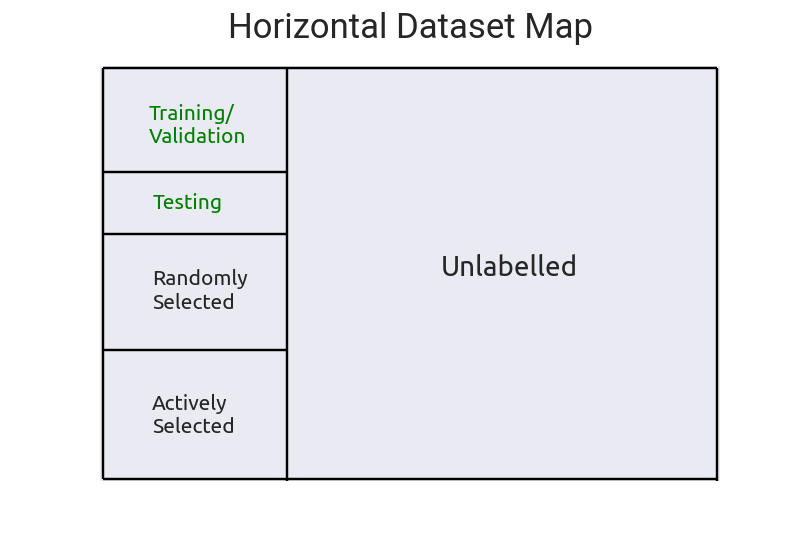
\includegraphics[width=.55\textwidth]{figures/chap5/dof/horizontal_dataset_map}
    \caption{Horizontal data set map}
    \label{c5:dataset_map}
\end{figure}

The distribution of cardinality in actively selected subset contained in the simulation pool is illustrated in Figure~\ref{c5:figure_active_distribution_densenet}.
Figures~\ref{c5:figure_active_cardinality_acc_densenet},~\ref{c5:figure_active_distribution_vgg} show the distribution of cardinality and accuracy from the simulation pool after a single query to DenseNet and VGG16 active learner respectively. 
We can observe that both classifiers perform similarly in terms of accuracy in individual confidence bins, but there is quite difference in cardinality.

A key point to mention is that we have selected the data solely on queries sent to DenseNet active learner and we also trained VGG16 with the already selected data, a similar method used in~\cite{bosser2020model}.
The assumption we made is that the simulation is agnostic to the label acquisition since our goal is to implement a fully automated active learning pipeline.

\begin{figure}[ht!]
    \centering  
    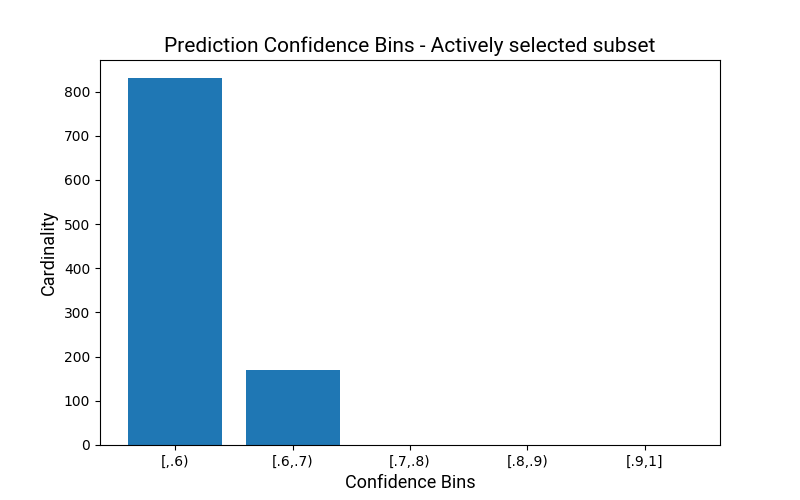
\includegraphics[width=.55\textwidth]{figures/chap5/simulation/pools/pred_conf_active_1000_dataset}
    \caption{Distribution of cardinalities in actively selected samples in prediction confidence bins for  actively selected sub pool (1000 samples)}
    \label{c5:figure_active_distribution_densenet}
\end{figure}

\begin{figure}[ht!]
    \centering  
    \subfigure[]{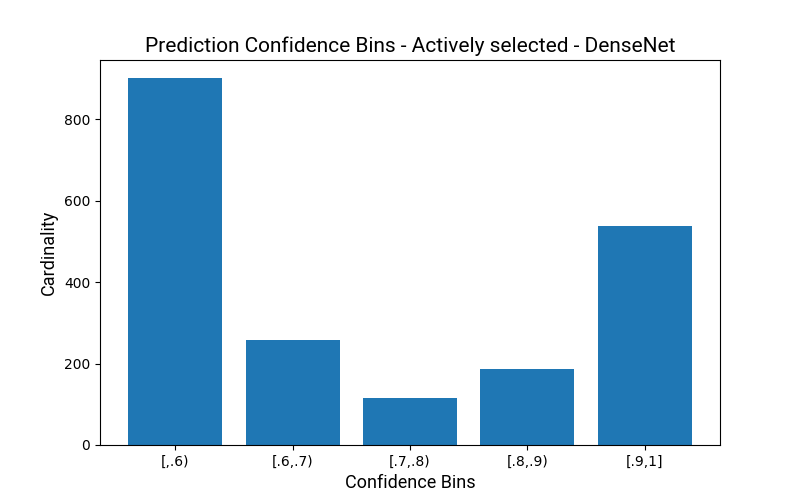
\includegraphics[width=.45\textwidth]{figures/chap5/simulation/pools/pred_conf_cardinality_pool_dataset_densenet}}
    \subfigure[]{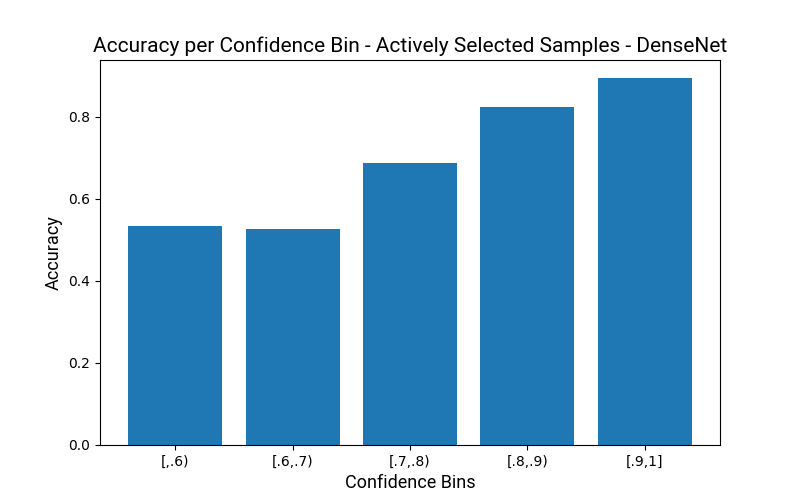
\includegraphics[width=.45\textwidth]{figures/chap5/simulation/pools/pred_conf_acc_active_densenet}}
    \caption{Distribution of actively selected samples in prediction confidence bins from DenseNet active learner: (a) cardinality (b) accuracy }
    \label{c5:figure_active_cardinality_acc_densenet}
\end{figure}

\begin{figure}[ht!]
    \centering  
    \subfigure[]{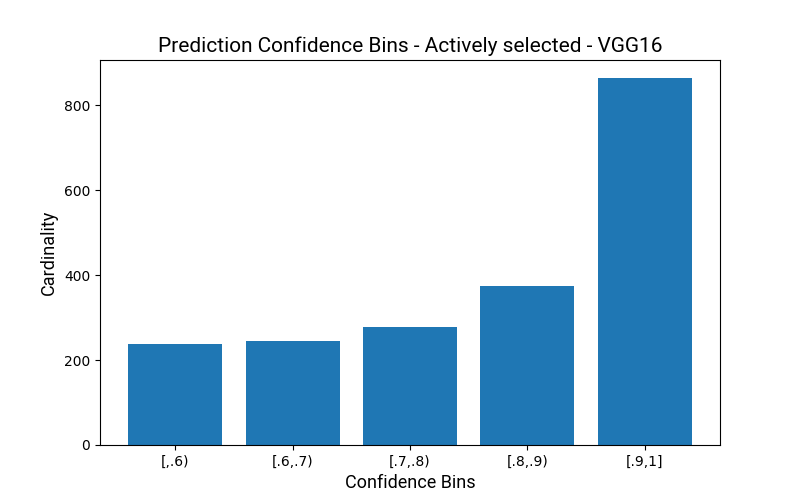
\includegraphics[width=.45\textwidth]{figures/chap5/simulation/pools/pred_conf_cardinality_pool_dataset_vgg}}
    \subfigure[]{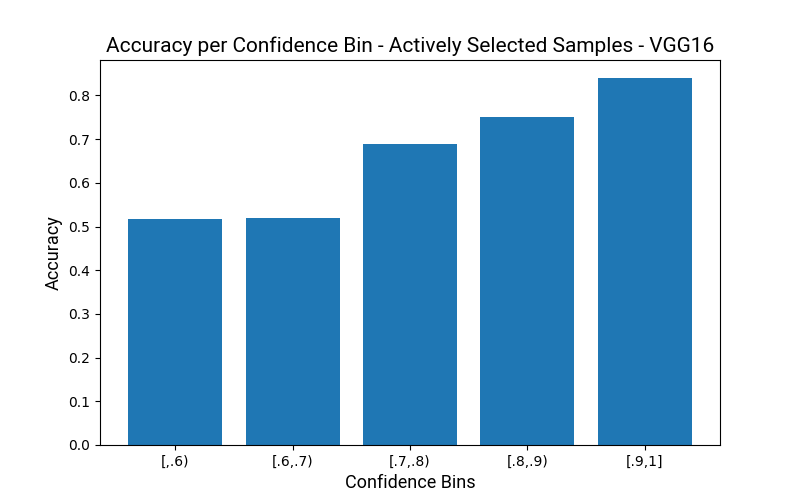
\includegraphics[width=.45\textwidth]{figures/chap5/simulation/pools/pred_conf_acc_active_vgg}}
    \caption{Distribution of actively selected samples in prediction confidence bins from VGG16 active learner: (a) cardinality (b) accuracy }
    \label{c5:figure_active_distribution_vgg}
\end{figure}


Finally, the pool dataset used for the simulation is comprised of 2000 annotated samples and is considered as new ``unknown'' data set for the simulation process.

The notion behind the simulation mode is to contradict random and active selection, running in parallel. Since a new batch represents a query to the active learner, we have already performed the query and annotation stage. Every next actively selected batch chosen by the current selection strategy, is added to the DoF labeled data set and the process is repeated until the pool is exhausted.


\subsection{Experimental setup}
\label{c5:section_experimental_setup}
Reviewing the literature, to the best of our knowledge there isn't a standard methodology for evaluating active learning algorithms with neural networks~\cite{gissin2019discriminative}. Our goal is to detect the most budget friendly and less time consuming method to obtain annotations. Thus, we are rather interested to fit the training set as well as possible by detecting those batches that will: a) maximise the classification accuracy with the less extra labelled examples, b) achieve the maximum overall performance, than creating a binary classifier with generalization in mind.

A single experiment for each active learning algorithm requires that the active learner is already queried on the experimental pool and responded with the LC measure in order to get the samples ranked in the pool.
In every intermediate step we train the model until convergence, and save the weights of the epoch with the best validation accuracy.
Finally, the test accuracy, f1-score and loss upon DoF test set, of the best model are recorded.
Performance results are drawn in curves, given the number of ``queried''-annotated instances.
The training process is set under a deterministic framework as described in Section~\ref{c5:section_passive_learning}, meaning that results are completely reproducible for the entire set of experiments, if the same seeds and hyperparameters are set.
However, training neural networks is still a stochastic process and in order to further reduce the variance from the results, each experiment ran 3 times, each one with a different seed of 0, 10 and 100.

Given the above and based on the methodologies and results of previous sections we end up with the following algorithms:

\begin{itemize}
 \item Random: a batch is chosen uniformly as in a regular ``passive'' supervised experiment.
 \item Single Query Active Learning(SQAL): Query the active learner once at the bootstrap stage, calculate the LC and use the same rank to pick the next batch throughout the entire experiment, until the pool is exhausted.
 \item Single Query Active Learning(SQAL) + CEAL: For the high confident $>$90\% based on LC predicted samples, use the predicted class as groundtruth.
 \item Active Learning Loop(ALL): Incrementally train and update the active learner parameters(weights and biases of the neural network) with the best recorded model of the new batch. Query the remaining samples of the pool and update their rank based on the LC. Pick the next batch upon the new rank.
 \item Active Learning Loop(ALL) + CEAL: For the high confident $>$90\% based on LC predicted samples, use the predicted class as groundtruth from the previous best recorded model.
\end{itemize}

The process for all the aforementioned active algorithms is visualised in Figures~\ref{c5:figure_al_ceal_single},~\ref{c5:figure_al_ceal_loop}.


\begin{figure}[ht!]
    \centering  
    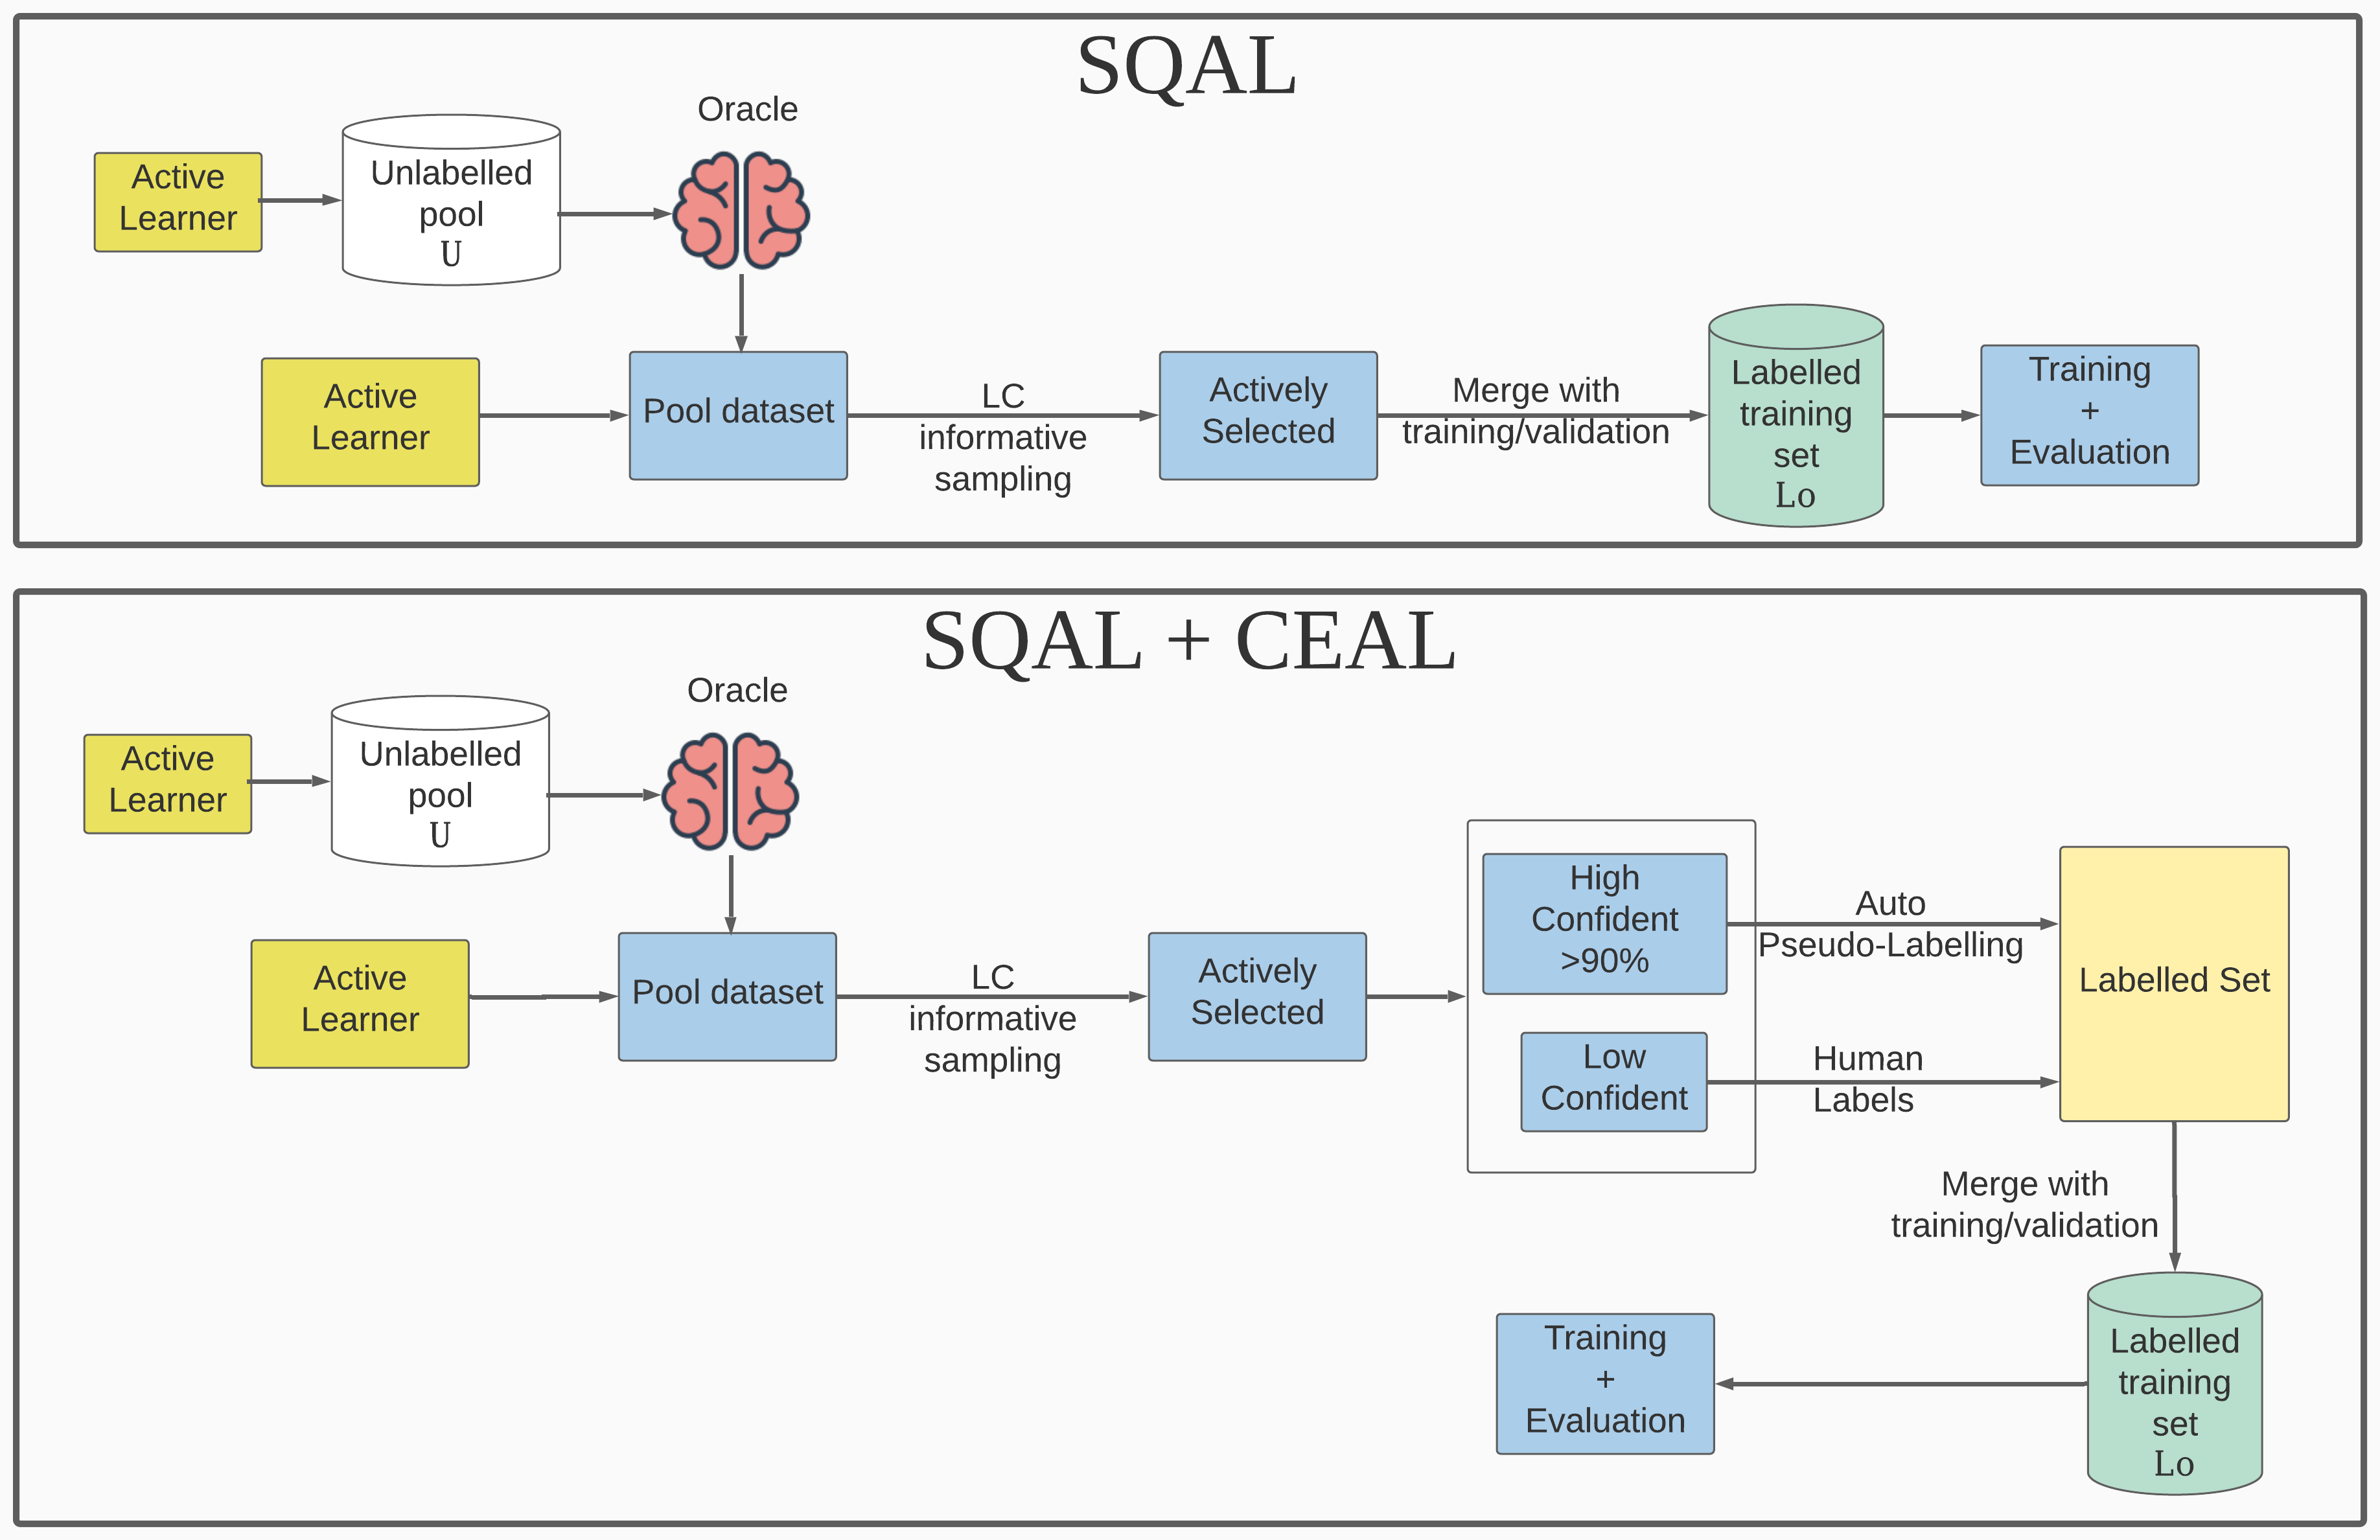
\includegraphics[width=\textwidth]{figures/chap5/al/al_sqal_ceal}
    \caption{Active Learning and CEAL single learning algorithm.}
    \label{c5:figure_al_ceal_single}
\end{figure}

\begin{figure}[ht!]
    \centering  
    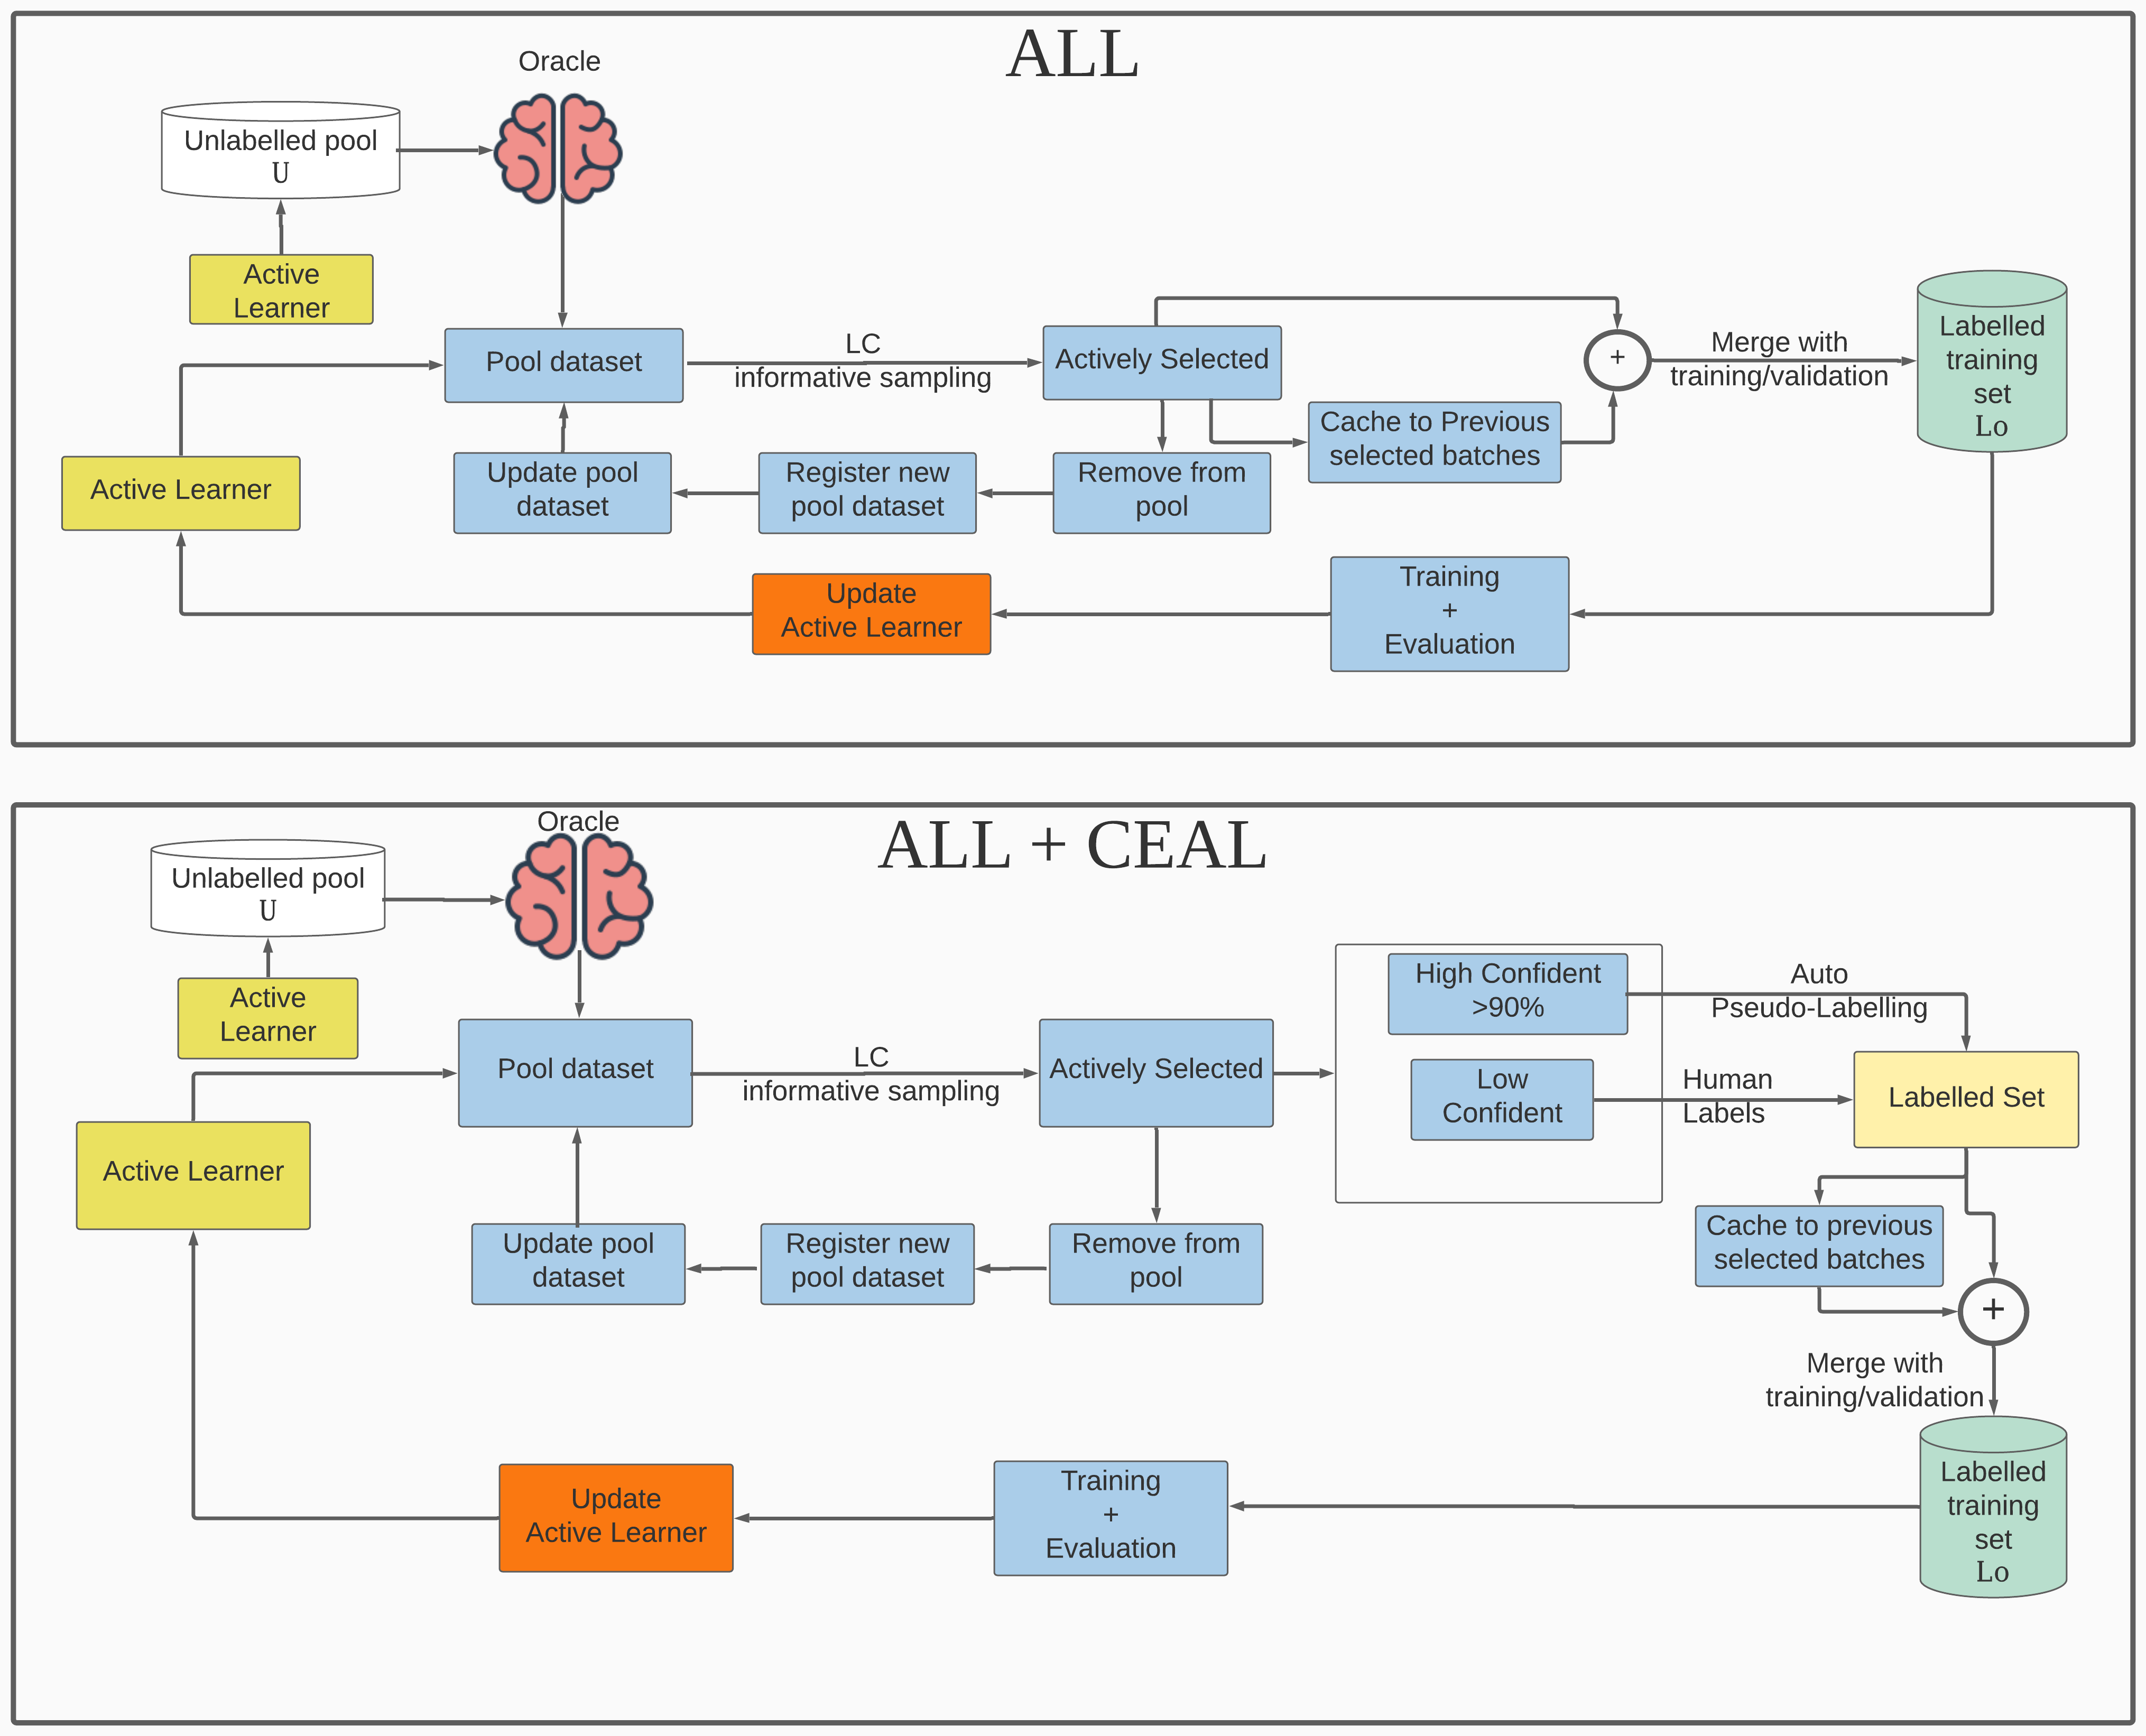
\includegraphics[width=\textwidth]{figures/chap5/al/al_all_ceal}
    \caption{Active learning and CEAL incrementally learning algorithm loop.}
    \label{c5:figure_al_ceal_loop}
\end{figure}


\subsection{Results - Performance}

For the simulation we evaluated two CNN based classifiers, a DenseNet trained from scratch and a pretrained VGG16, on 5 different algorithms.
We measured the classification accuracy, F1-score macro and loss and reported the mean values from 3 distinct runs each one with a unique random seed, on the best performed model in every experiment.

Figures~\ref{c5:figure_simulation_acc_densenet_vgg},~\ref{c5:figure_simulation_loss_densenet_vgg} visualise the measured accuracy/F1-score performance and loss for DenseNet and VGG16 respectively, for all algorithms.

\begin{figure}[h!]
    \centering  
    \subfigure[]{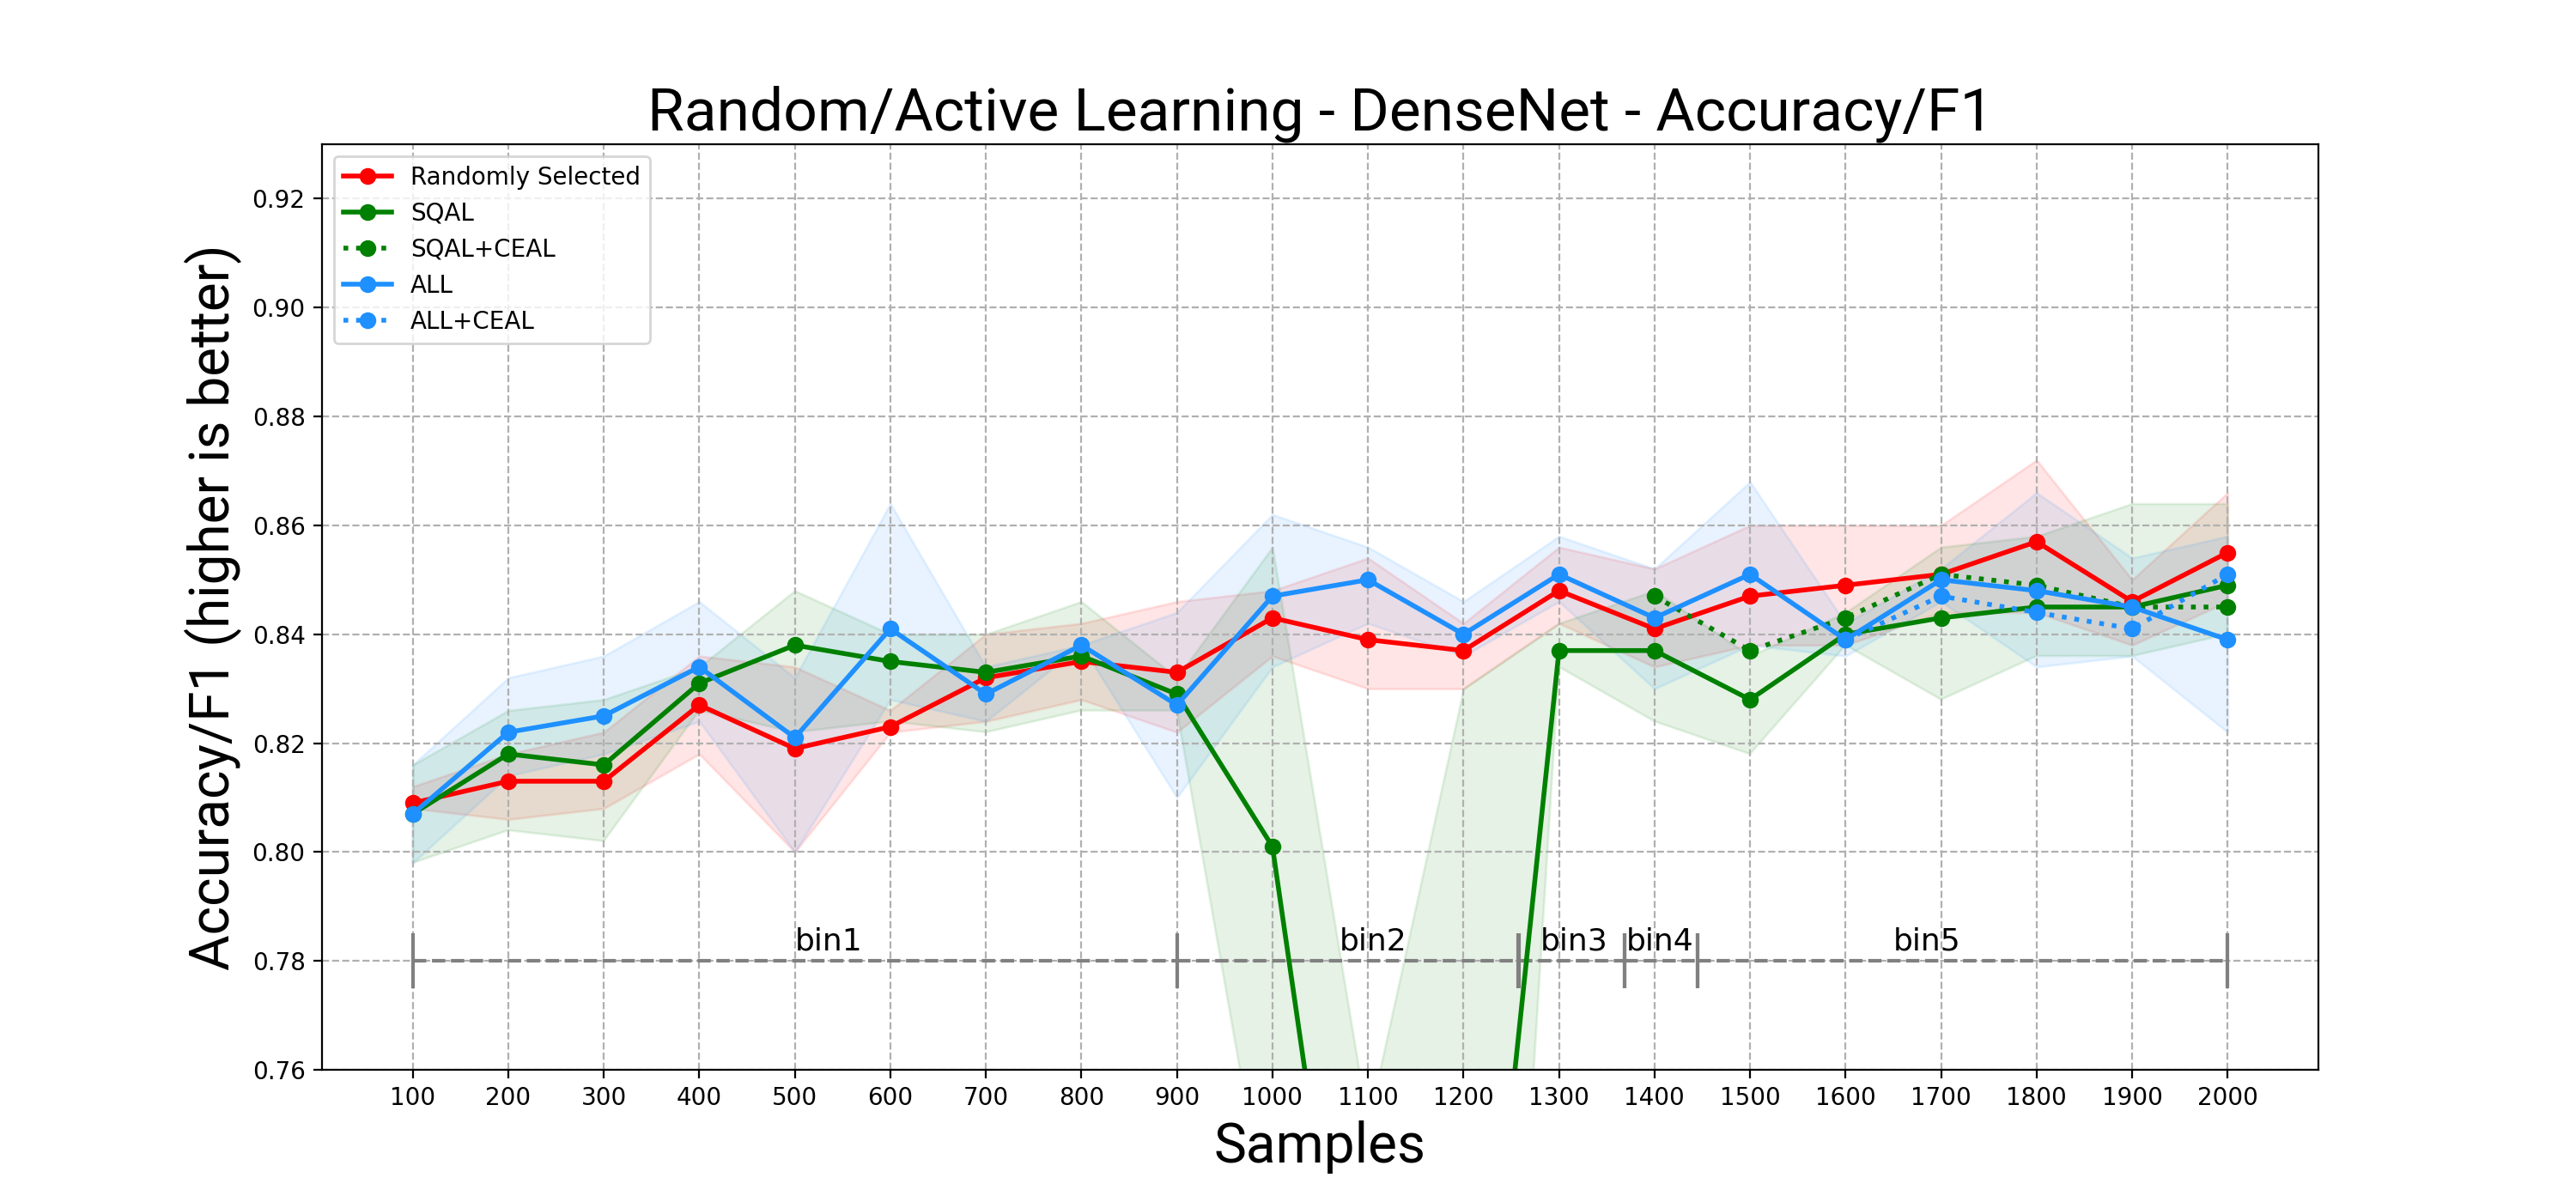
\includegraphics[width=1\textwidth]{figures/chap5/simulation/charts/simulation_accuracy_densenet}}
    \subfigure[]{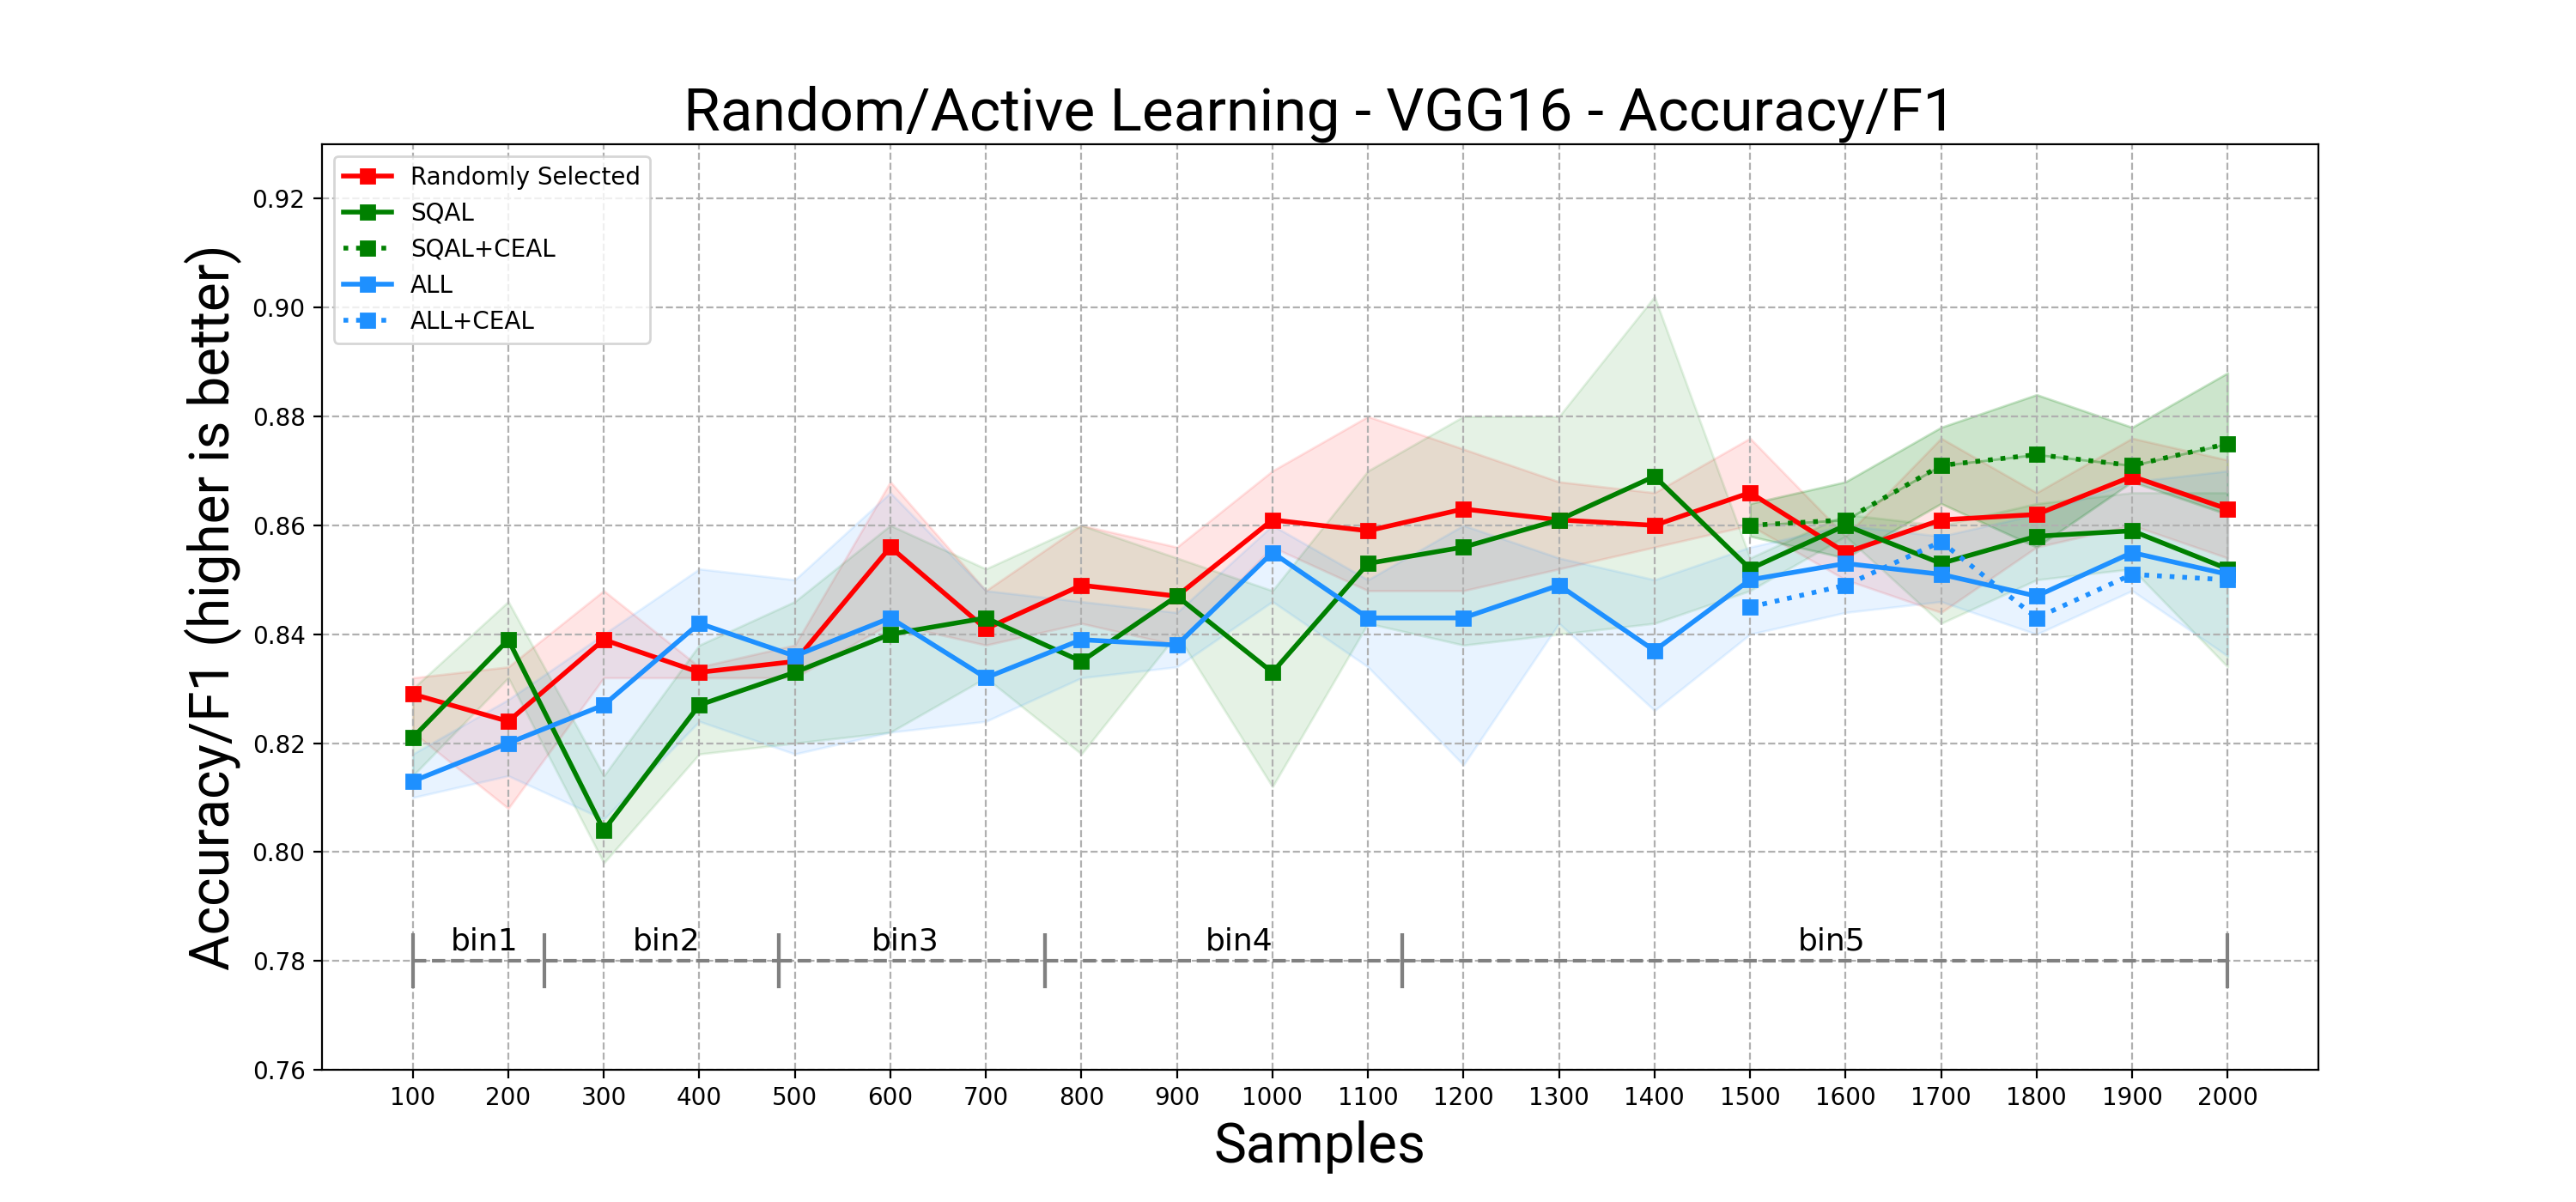
\includegraphics[width=1\textwidth]{figures/chap5/simulation/charts/simulation_accuracy_vgg}}
    \caption{Accuracy/F1 plots of the different algorithms for the DoF active learning experiments. The results are averaged and the coloured area is the performance deviations from the minimum to the maximum recorded value: (a) DenseNet, (b) VGG16}
    \label{c5:figure_simulation_acc_densenet_vgg}
\end{figure}

Bellow the charts, the ``ruler'' with confidence bin margins, is related only with SQAL algorithm and denotes the corresponded confidence bin that the current pool batch participates. On the other hand, concerning ALL algorithm the equivalent batch participation is shown in Figures~\ref{c5:figure_al_loop_participation_densenet},~\ref{c5:figure_al_loop_participation_vgg}.

Concerning DenseNet, a clear initial observation on the results is that almost until the final batch of the lowest confidence \textit{bin1} both active learning algorithms outperform random sampling. Concerning ALL algorithm, it shows a more consistent performance and dominates over the random selection whereas SQAL does not perform well when more confident observations are included in dataset.

As we have mentioned in Section~\ref{c5:section_active_learning_indicator} we are dealing with the rarity of low confidence samples due to the over confident prediction nature of neural networks. This seems that it could be a beneficial factor for DenseNet model as the performance for ALL algorithm is initially maximised in 6th batch (600 queried/annotated samples) and peaks at the 15th batch with no significant difference.
In addition, the rate in performed accuracy until the 4th batch, is significantly higher that the random selection and SQAL, another reason to consider that given a larger volume of borderline queries ALL method have potential for even faster performance increase.

On the other hand, random sampling outperforms the other two at the 18th batch, with almost all the available annotated instances, participating in the training set.

In parallel, the performance for CEAL experiments cannot be left unnoticed. In SQAL, CEAL (green-dotted) outperforms the same algorithm (green-solid) with the real groundtruth while it performs similarly to random selection, given that almost 10\% of the pseudo-labelled instances are false. % insight we can use this instead of annotating

% about underfit 
Concerning te SQAL algorithm, it is worth mentioning that as more confident samples are added in the training set, approximately from 1000 samples and above, model underfits on training set, with almost 10\% deviation between training and validation accuracy, meaning that the model complexity is inadequate to fit the data properly.
In batches 1000-1200, it completely fails to fit and its performance is poor.

This effect though is completely absent in ALL algorithm and fitting were regular in most of the experiments with tolerant amount of overfit or any overfit at all.

Though, the option of tuning the parameters when a new batch arrives, is not possible for a couple of reasons. We focus in a data-driven performance improvement method while during a fully automated process hyperparameter tuning is not possible.

%%%%%%%%%%%%%%%%%%%%%%% VGG %%%%%%%%%%%%%%%%%

In experiments with pretrained VGG16 model in Figure~\ref{c5:figure_simulation_acc_densenet_vgg}(b),~\ref{c5:figure_simulation_loss_densenet_vgg}(b), an initial observation tells that all algorithms increase their performance as batches progress, though there isn't a consistent winner.
For the most of batches random selection outperforms the others.

\begin{figure}[h!]
    \centering  
    \subfigure[]{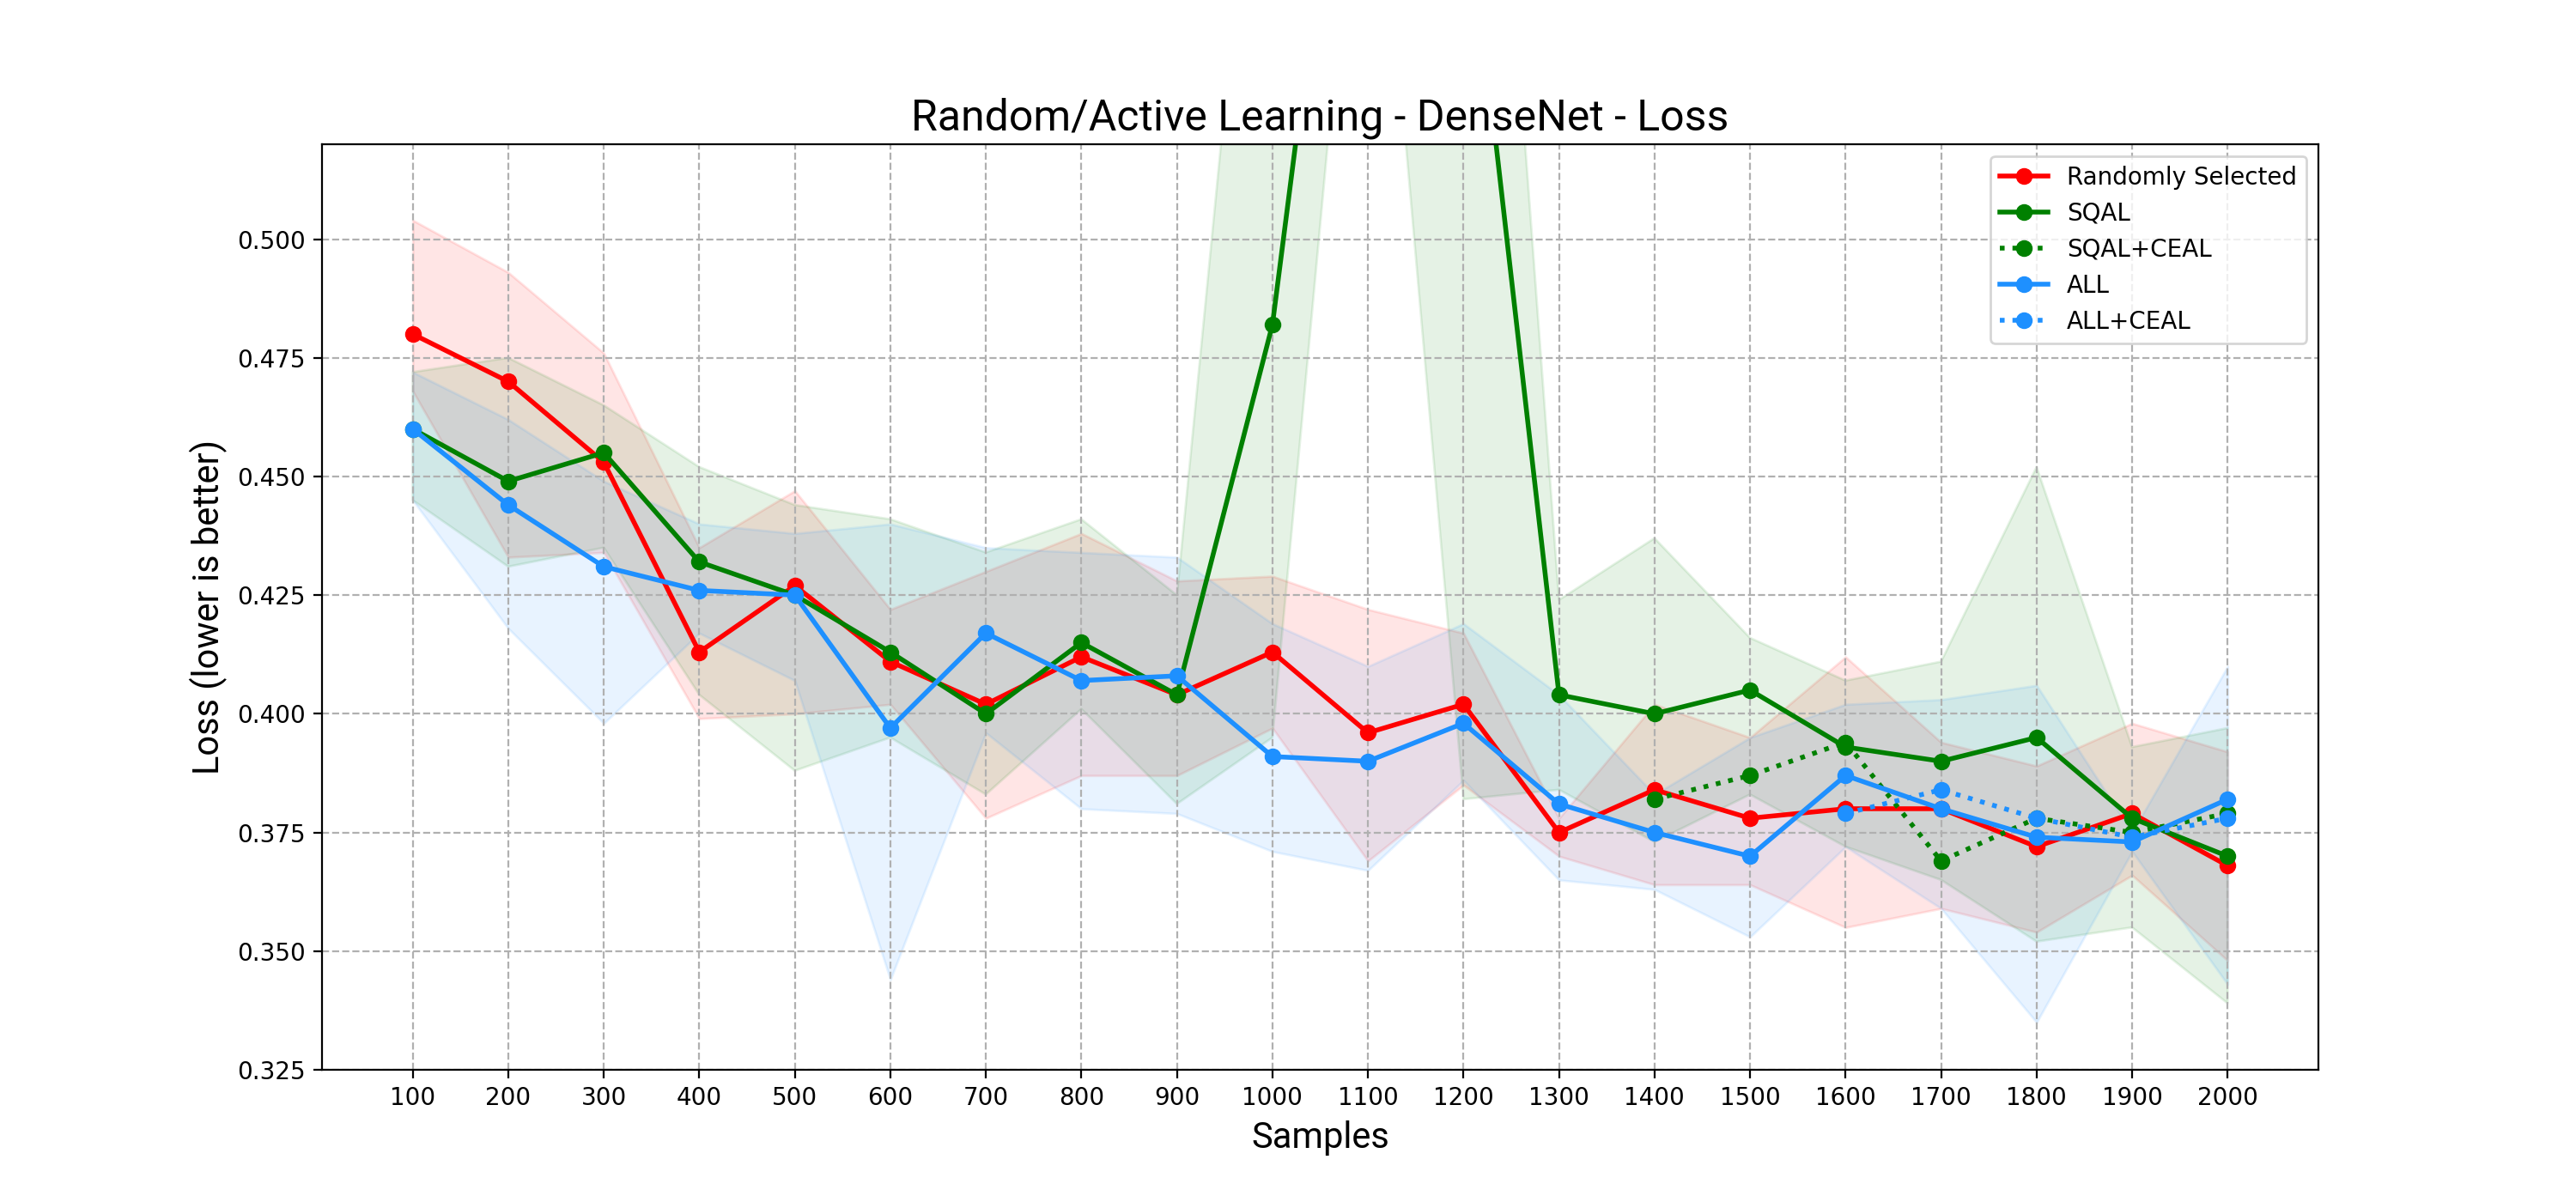
\includegraphics[width=1\textwidth]{figures/chap5/simulation/charts/simulation_loss_densenet}}
    \subfigure[]{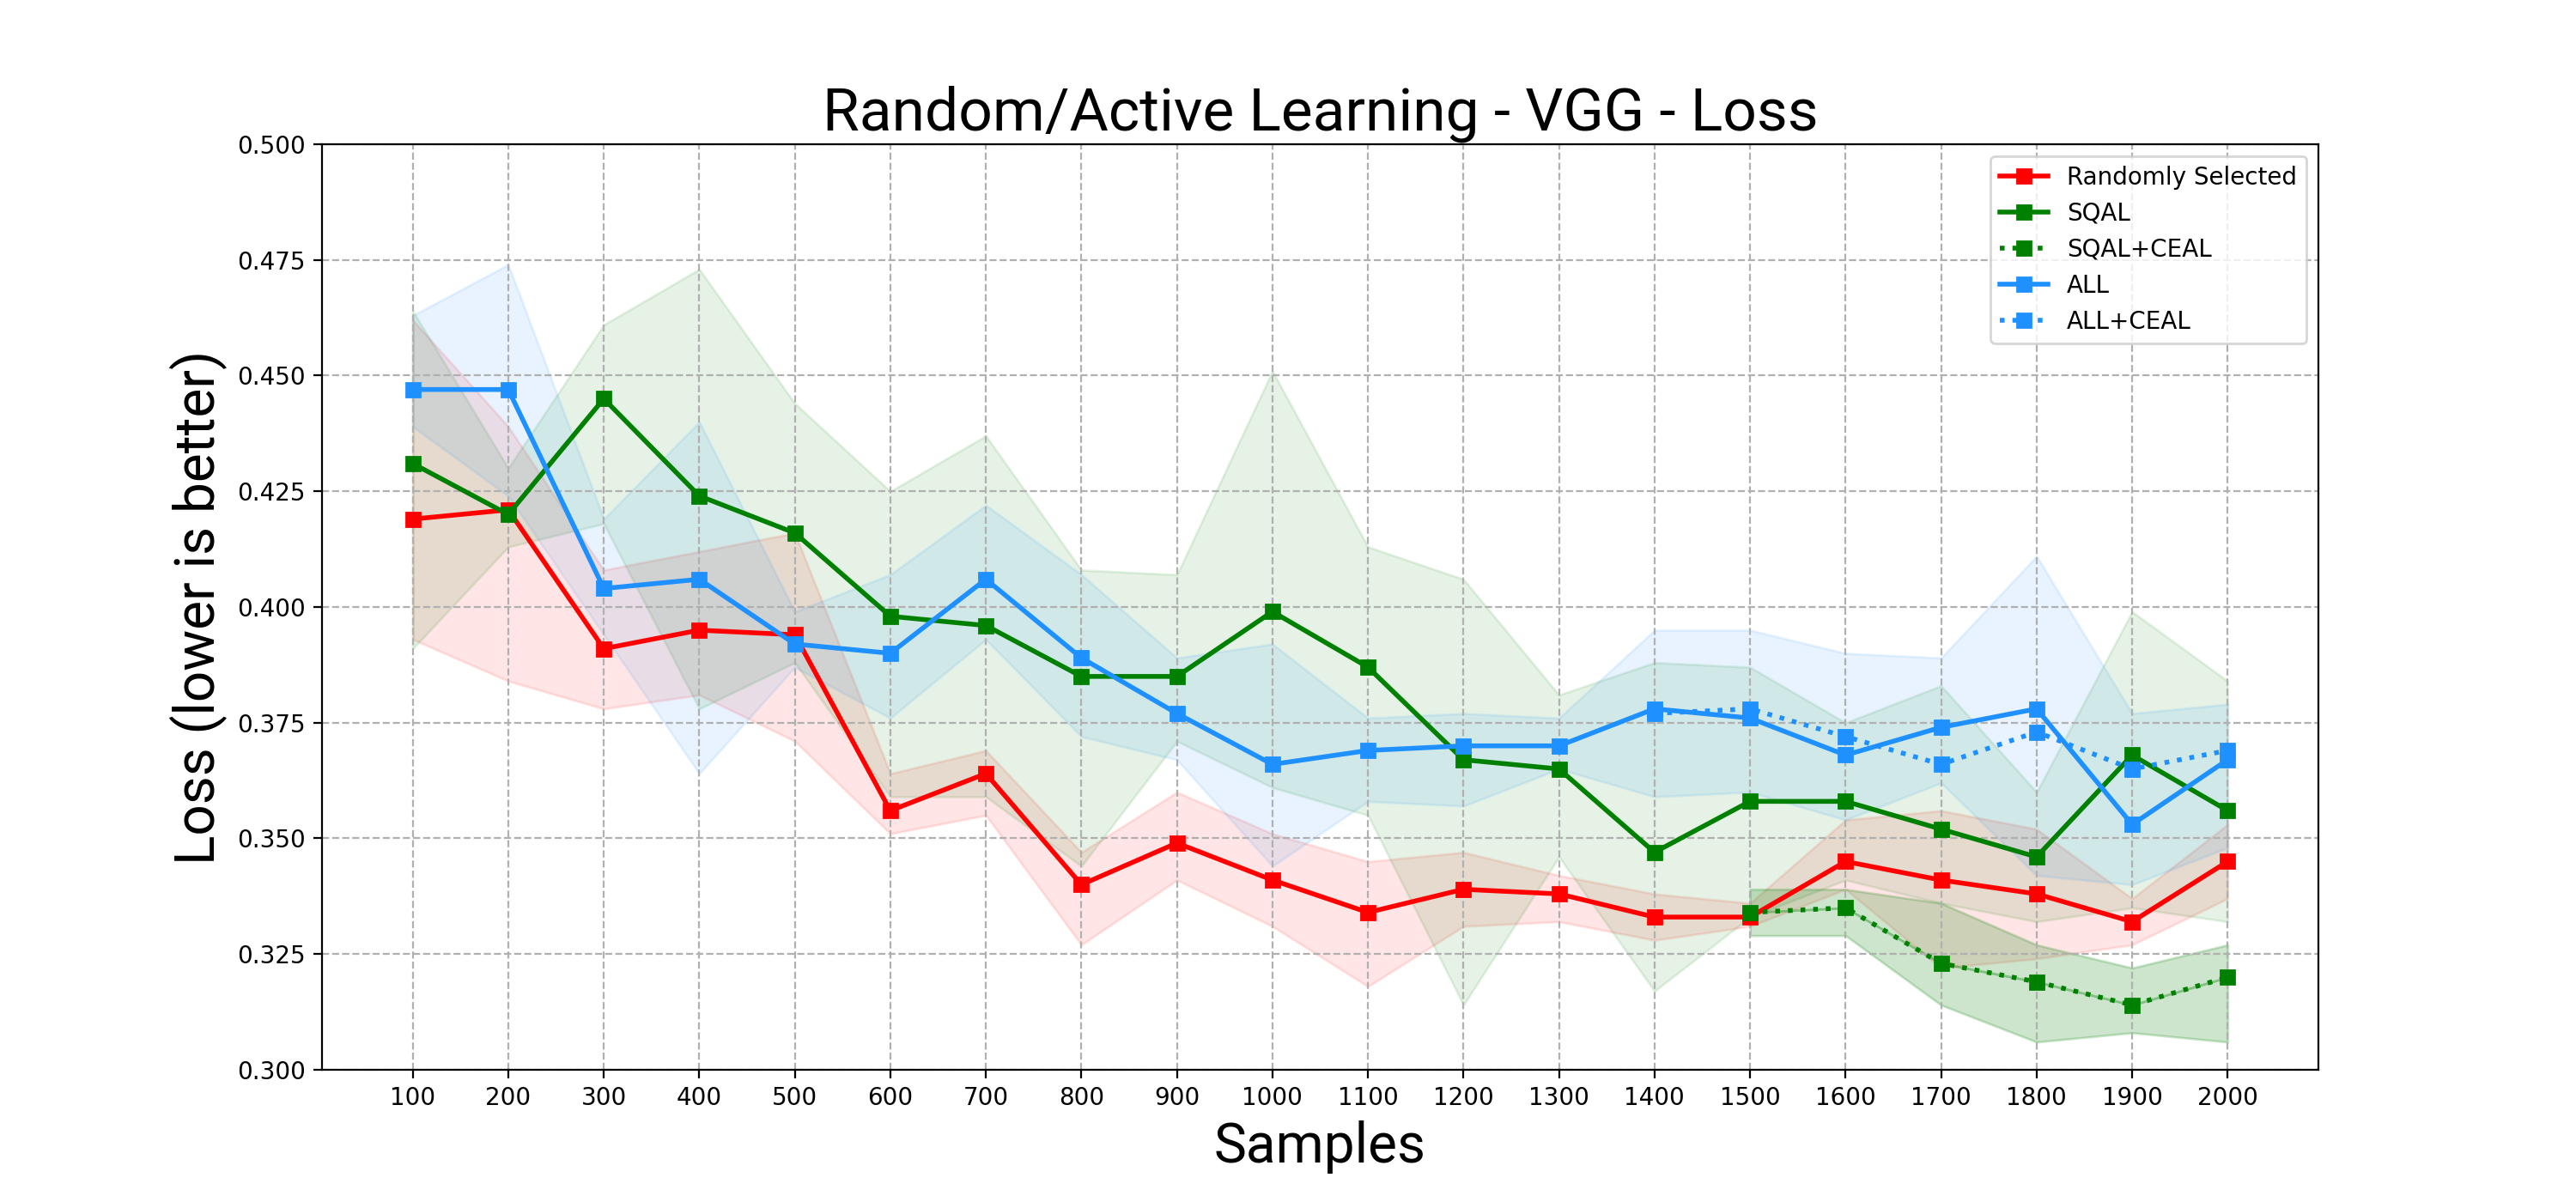
\includegraphics[width=1\textwidth]{figures/chap5/simulation/charts/simulation_loss_vgg}}
    \caption{Loss of the different algorithms for the DoF active learning experiments. The results are averaged and the coloured area is the standard deviations: (a) DenseNet, (b) VGG16}
    \label{c5:figure_simulation_loss_densenet_vgg}
\end{figure}


SQAL is the most inconsistent but it peaks higher than other settings in the 14th batch. In addition, an unexpected behavior can be observed in SQAL + CEAL setting, where it clearly outperforms the rest with almost with +5\% accuracy deviation in some cases. It is an obvious domination for CEAL algorithm when pseudolabelling the groundtruth with the predicted classes, in instances with $>90\%$ confidence from VGG16 active learner.

%%%%%%%%%% all %%%%%%%%%%%%%%%%%%

Figure~\ref{c5:figure_simulation_acc_loss_all} illustrates the performed mean values for accuracy/F1-score and loss among all algorithms and classifiers from the three runs, where circle points represent DenseNet experiments and square points VGG16. Dotted charts visualise only the CEAL settings for both classifiers.

Comparing the experiments in total, VGG16 outperforms DenseNet in recorded accuracy/F1-score in most of the algorithms. The winner setting is the SQAL+CEAL algorithm where outperforms all the others in the final batch, without any substantial gain from same classifier in SQAL in 14th batch.


\begin{figure}[h!]
    \centering  
    \subfigure[]{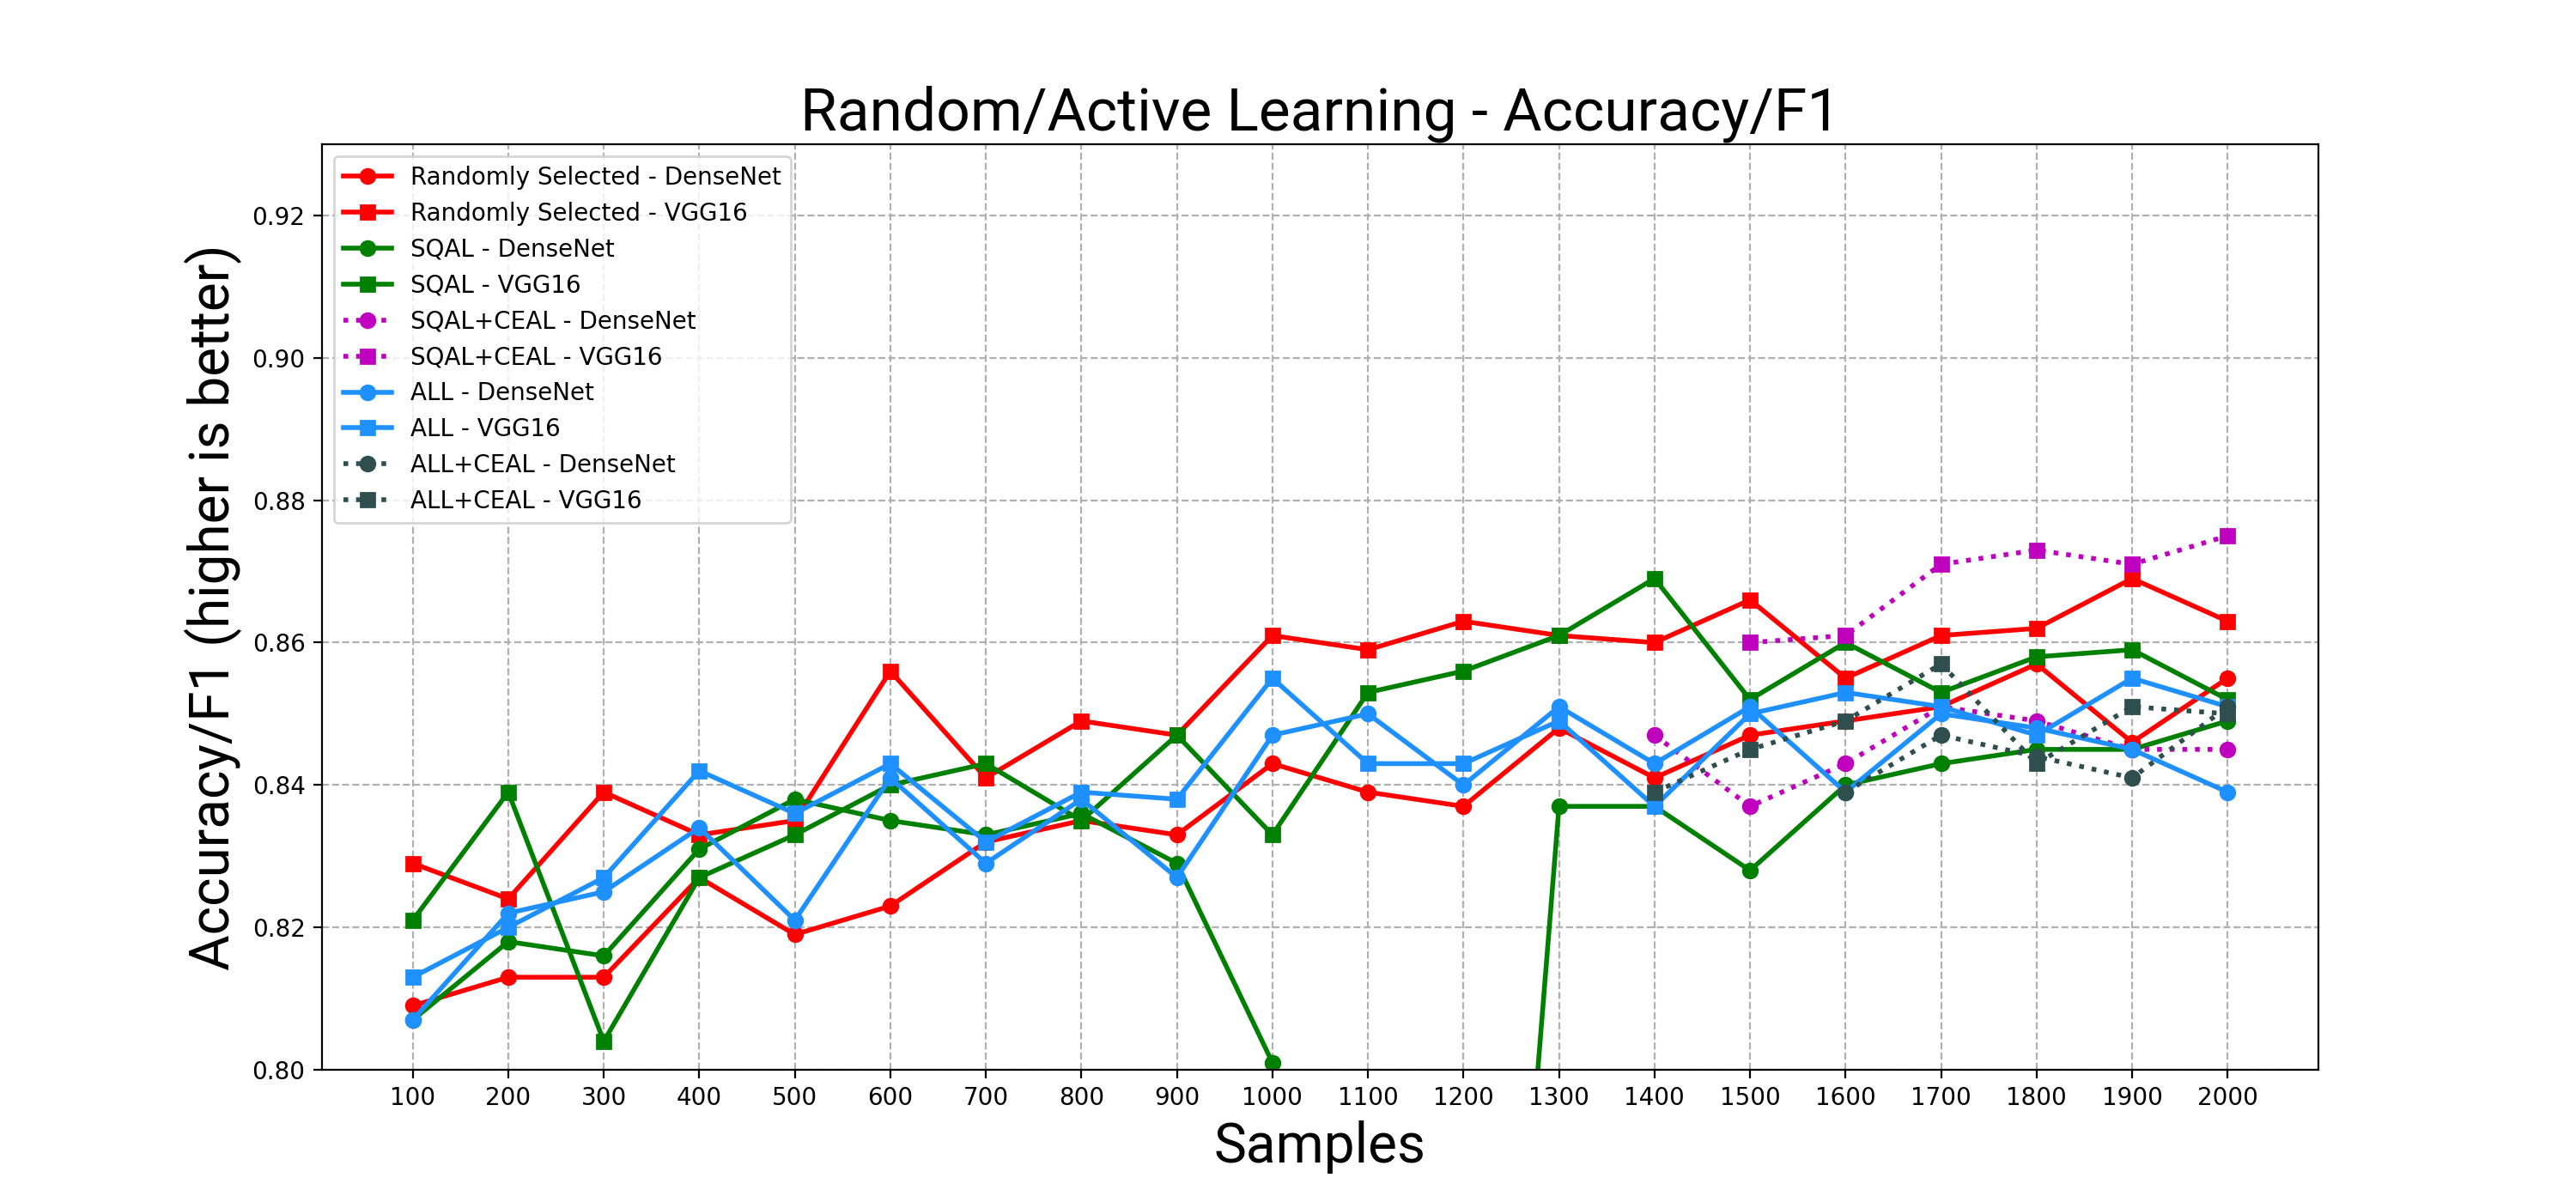
\includegraphics[width=1\textwidth]{figures/chap5/simulation/charts/simulation_accuracy_all}}
    \subfigure[]{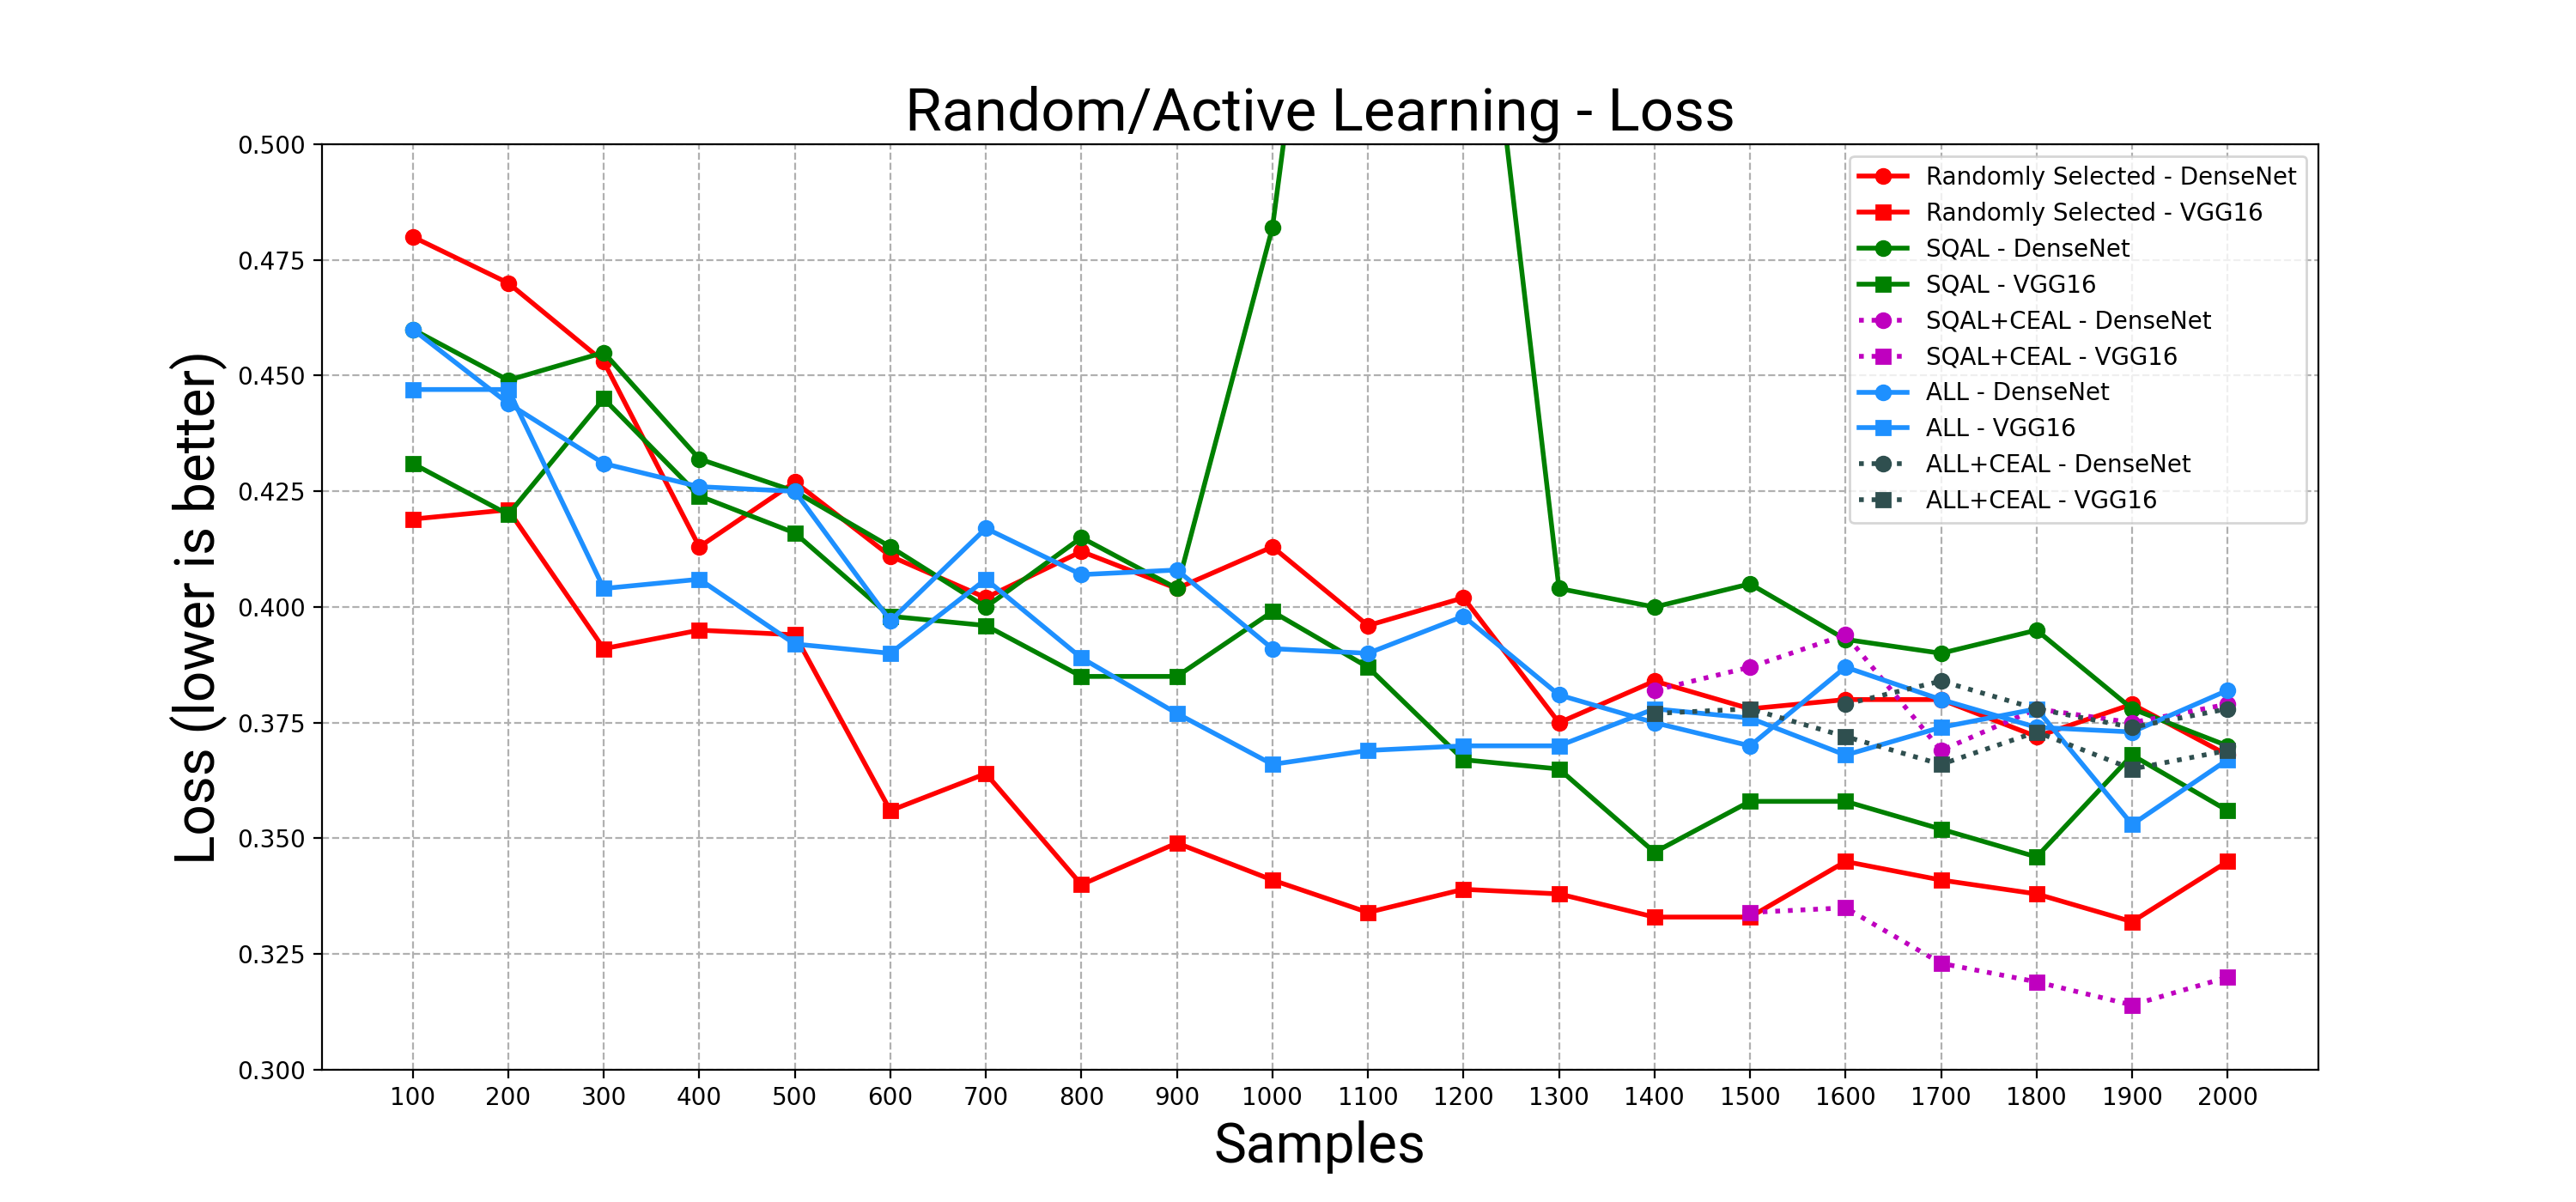
\includegraphics[width=1\textwidth]{figures/chap5/simulation/charts/simulation_loss_all}}
    \caption{Measured mean accuracy/f1-score and loss for all experiments in Random, Active and CEAL for single and loop settings: (a) Accuracy/F1-score, (b) Loss}
    \label{c5:figure_simulation_acc_loss_all}
\end{figure}

Table~\ref{c5:table_experiment_performance_table} shows the recorded performance in random and active settings. More specifically, we provide the maximum recorded value for k10 and k20 samples and minimum k20 samples.
As we mentioned in a previous section, our goal is to find the setting which performs higher minimizing the number of queries to the oracle.
Our findings for the experiments show that within the first 10 batches (1000 annotations), the highest accuracy is 87\% for random selection using VGG16 architecture. Nevertheless, in 6th batch, the ALL setting for both classifiers performs quite close in 86.6\% (VGG16), 86.4\% (DenseNet) and given the extra budget of 400 annotation we can assume that the difference is not substantial.
Given all the available annotated k20 batches the highest recorded accuracy is 90.2\%, performed by SQAL setting with VGG16 model with 14 annotated batches. Given the performance margin, the difference in the annotation budget can be considered rational and in performance substantial. In addition given the architecture properties of VGG16 which has almost $3850\times$ the parameters of DenseNet model configuration of this work, this comes with the tradeoff of the time needed to train the network even though we have freezed the pretrained module.


\begin{table}[ht!]
\centering
\footnotesize
\begin{tabular}{c|c|c|c|c}

\multicolumn{1}{c|}{} & \multicolumn{1}{c|}{Setting - Model} & \multicolumn{1}{c|}{Maximum-k10} & \multicolumn{1}{c|}{Maximum-20} & \multicolumn{1}{c}{Minimum-k20} \\ \hline

\multirow{2}{*}{Random} & DenseNet & 84.8/10  & 87.1/18 & 80/5  \\
                        & VGG16    & \textbf{87/10}    & \textbf{88/11} & 81/2  \\ \hline

\multirow{8}{*}{Active} & SQAL - DenseNet & 85.6/10 & 87.2/18 & 55/12  \\
                        & SQAL - VGG16    & 86/6    & \textbf{90.2/14} & 79.8/3  \\ \cline{2-5}
                        & SQAL + CEAL - DenseNet & -& 84.7/17 & 82.2/15  \\ 
                        & SQAL + CEAL - VGG16 & - & \textbf{88.8/20} & 85.8   \\ \cline{2-5}
                        & ALL - DenseNet & \textbf{86.4/6} & 86.7/15 & 79.9/1 \\
                        & ALL - VGG16    & \textbf{86.6/6} & 86.6/6 & 81/1  \\ \cline{2-5}
                        & ALL + CEAL - DenseNet &- & 85.7/17 & 83.4/16   \\
                        & ALL + CEAL - VGG16 &- & 86.8/17 & 84/18  \\ \hline
\end{tabular}
\caption{Maximum and minimum recorded performance for k10 and k20  batch for all experiments.}
\label{c5:table_experiment_performance_table}
\end{table}

\begin{figure}[ht!]
    \centering  
    \subfigure[]{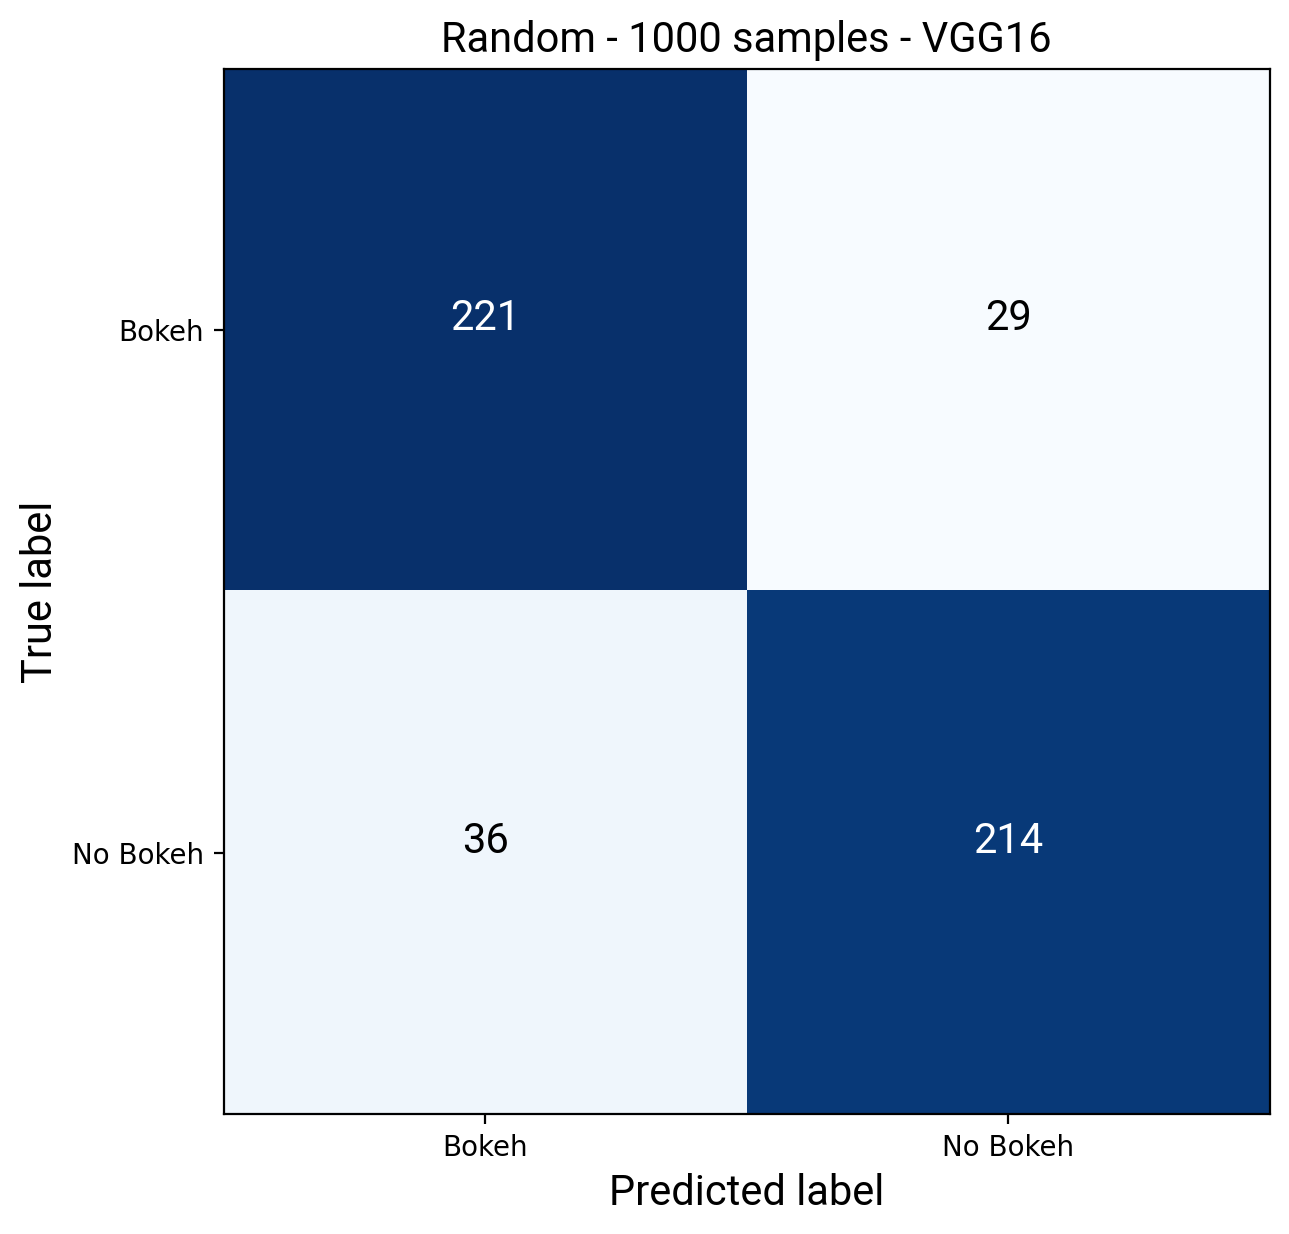
\includegraphics[width=.3\textwidth]{figures/chap5/simulation/cm/random/vgg_random_1000_cm}}
    \subfigure[]{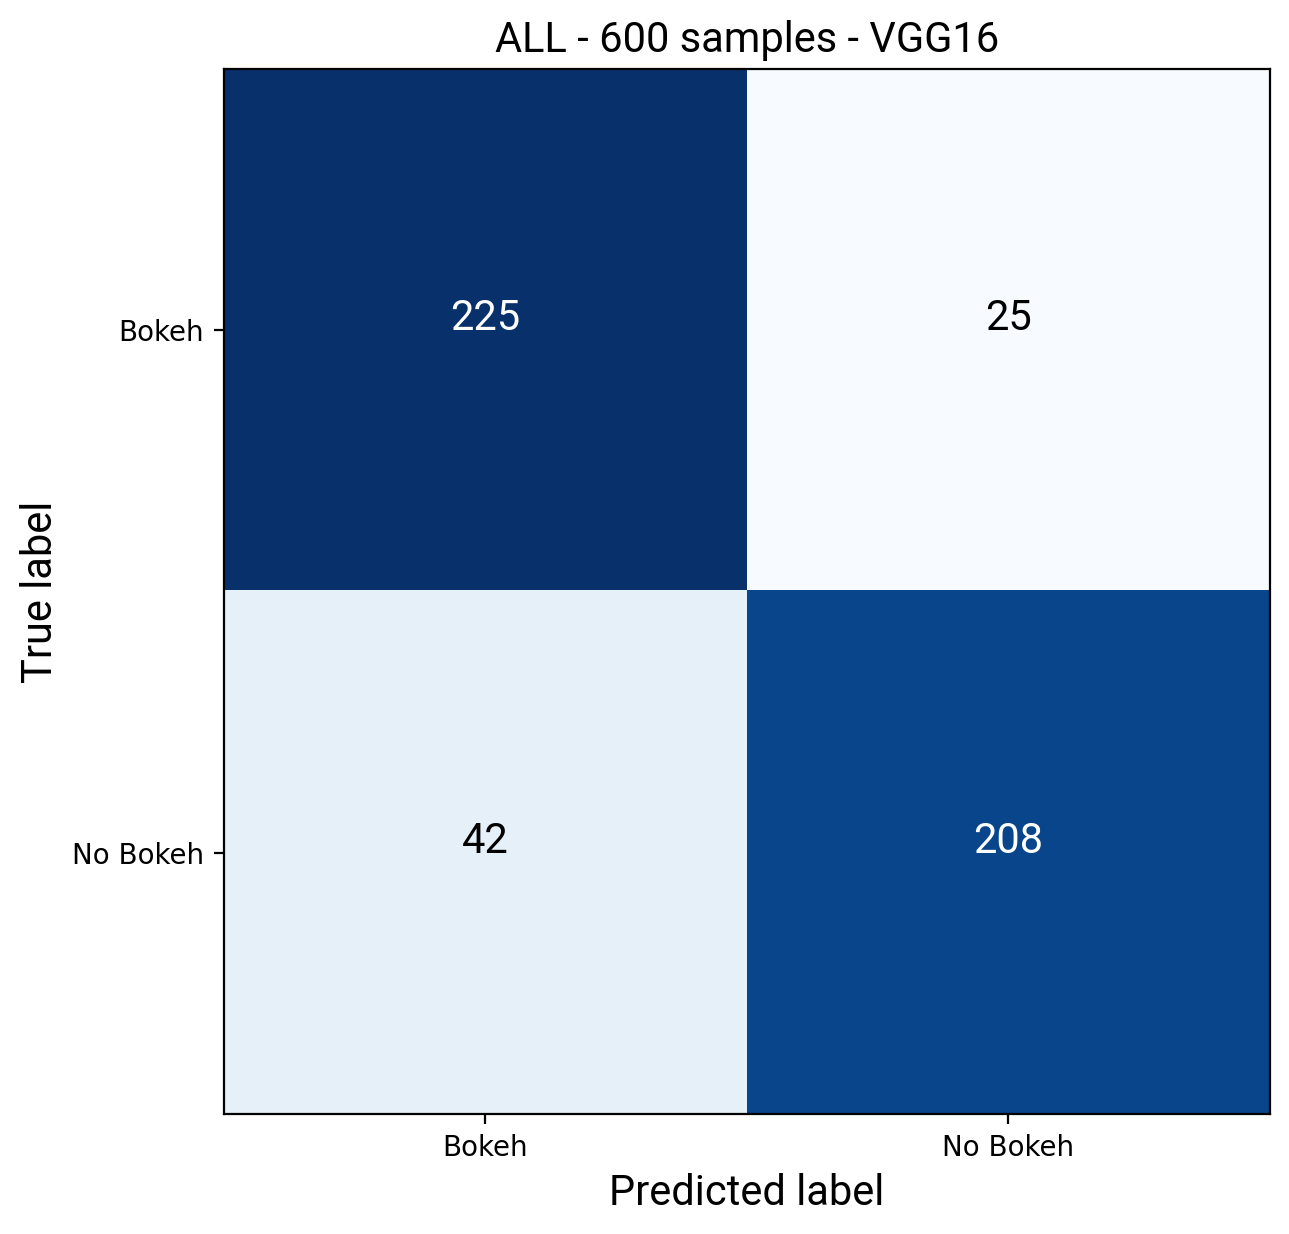
\includegraphics[width=.3\textwidth]{figures/chap5/simulation/cm/active/vgg_all_600_cm}}
    \subfigure[]{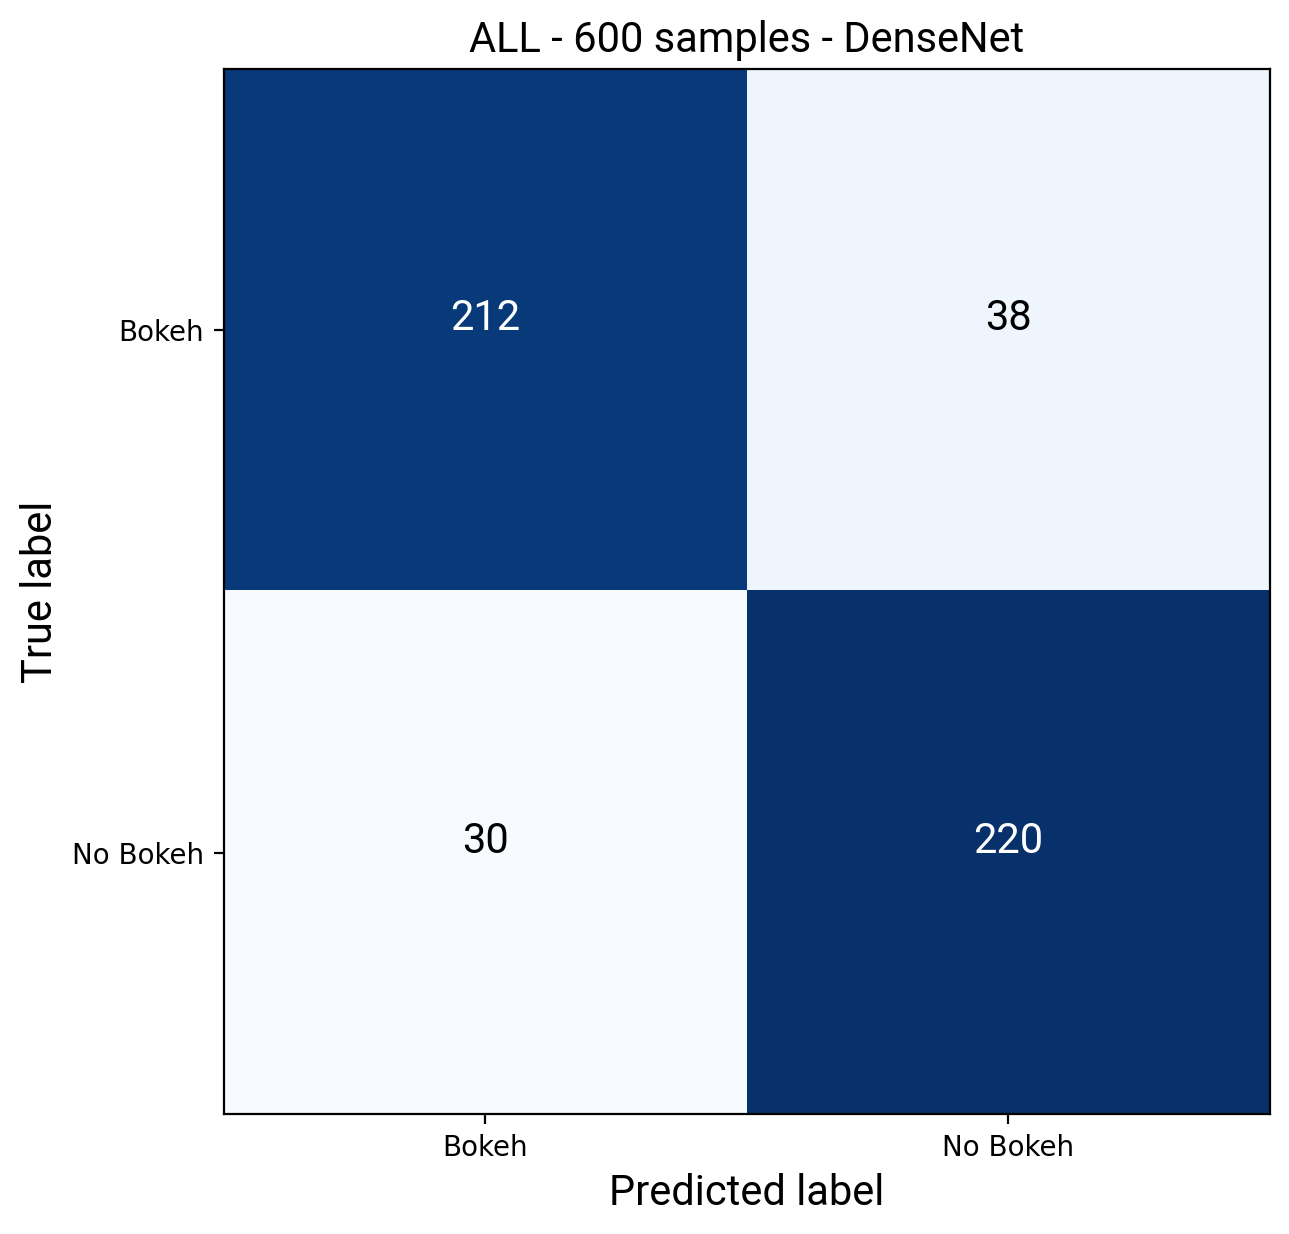
\includegraphics[width=.3\textwidth]{figures/chap5/simulation/cm/active/densenet_all_600_cm}}
    \caption{Confusion matrices of the top k10 best recorded runs in simulation experiments: (a) random-vgg16, (b) ALL-VGG16, (c) ALL-DenseNet.}
    \label{c5:figure_cm_k10}
\end{figure}

\begin{figure}[ht!]
    \centering  
    \subfigure[]{\includegraphics[width=.3\textwidth]{figures/chap5/simulation/cm/random/vgg_random_1100_cm}}
    \subfigure[]{\includegraphics[width=.3\textwidth]{figures/chap5/simulation/cm/active/vgg_sqal_1400_cm}}
    \subfigure[]{\includegraphics[width=.3\textwidth]{figures/chap5/simulation/cm/active/vgg_sqal_ceal_2000_cm}}
    \caption{Confusion matrices of the top k20 best recorded runs in simulation experiments: (a) random-vgg16, (b) SQAL-VGG16, (c) SQAL-CEAL-VGG16.}
    \label{c5:figure_cm_k20}
\end{figure}


\subsection{Results - Confidence Participation}

The key difference between SQAL and ALL algorithms is that for the latter the active learner is trained incrementally and is updated during the current run, the remaining samples in the pool are re-queried and consequently their rank is updated based on prediction confidence. Then the next batch is picked and so forth.

A family of plots relative with the confidence bin sample participation concerning ALL algorithm is provided in Figures~\ref{c5:figure_al_loop_participation_densenet}-~\ref{c5:figure_al_loop_pseudolabels_participation_vgg}. The sample participation heatmap per bin, is equivalent to the ``ruler'' in Figure~\ref{c5:figure_simulation_acc_densenet_vgg} and shows and percentage of samples per confidence bin, participating in the current selection from simulation data pool.

It would be interesting to compare the margins in confidence bins between the two methods. Figure~\ref{c5:figure_al_loop_participation_densenet} visualise the participation for the three individual experiments per seed and in comparison with Figure~\ref{c5:figure_simulation_acc_densenet_vgg}, we can observe that the margins are quite different. For example in SQAL algorithm \textit{bin1} participates until the 9th batch, whereas in ALL is depleted in 6th.

Similar condition is observed for the most confident \textit{bin5}, where in SQAL experiments starts from the 15th batch while in ALL starts from 17th and 18th depending the run.
Intuitively this can be justified by the experiment progression where in every training cycle, a new classifier is generated on a pool of queried samples where the classification boundary is most uncertain. 
As the algorithm learns to fit the less confident samples, classification boundary is improved and so forth active learner produces becomes more certain when queried on the remaining samples.

In Figures~\ref{c5:figure_al_loop_pseudolabels_participation_densenet},~\ref{c5:figure_al_loop_pseudolabels_participation_vgg}, heatmaps of CEAL algorithms show a minor change between the non CEAL method. It can be assumed that pseudolabelling does not contribute negatively for the next batch estimation.




\begin{figure}[h!]
    \centering
    \subfigure[]{\includegraphics[width=.32\textwidth]{figures/chap5/simulation/participation/densenet/participation_production_0}}
    \subfigure[]{\includegraphics[width=.32\textwidth]{figures/chap5/simulation/participation/densenet/participation_production_10}}
    \subfigure[]{\includegraphics[width=.32\textwidth]{figures/chap5/simulation/participation/densenet/participation_production_100}}
    %\includegraphics[width=9cm]{figures/chap5/simulation/participation/densenet/participation_production_0}
    \caption{DenseNet - ALL - Confidence bin participation per actively selected batch in training round: (a) seed=0, (b) seed=10, (c) seed=100.}
    \label{c5:figure_al_loop_participation_densenet}
\end{figure}


\begin{figure}[h!]
    \centering
    \subfigure[]{\includegraphics[width=.32\textwidth]{figures/chap5/simulation/participation/vgg/participation_production_0}}
    \subfigure[]{\includegraphics[width=.32\textwidth]{figures/chap5/simulation/participation/vgg/participation_production_10}}
    \subfigure[]{\includegraphics[width=.32\textwidth]{figures/chap5/simulation/participation/vgg/participation_production_100}}
    %\includegraphics[width=9cm]{figures/chap5/simulation/participation/densenet/participation_production_0}
    \caption{VGG16 - ALL - Confidence bin participation per actively selected batch in training round: (a) seed=0, (b) seed=10, (c) seed=100.}
    \label{c5:figure_al_loop_participation_vgg}
\end{figure}


\begin{figure}[h!]
    \centering
    \subfigure[]{\includegraphics[width=.31\textwidth]{figures/chap5/simulation/participation/densenet/participation_production_augmented_0}}
    \subfigure[]{\includegraphics[width=.31\textwidth]{figures/chap5/simulation/participation/densenet/participation_production_augmented_10}}
    \subfigure[]{\includegraphics[width=.31\textwidth]{figures/chap5/simulation/participation/densenet/participation_production_augmented_100}}
    %\includegraphics[width=9cm]{figures/chap5/simulation/participation/densenet/participation_production_0}
    \caption{DenseNet - ALL + CEAL - Confidence bin participation per actively selected batch in training round: (a) seed=0, (b) seed=10, (c) seed=100.}
    \label{c5:figure_al_loop_pseudolabels_participation_densenet}
\end{figure}


\begin{figure}[ht!]
    \centering
    \subfigure[]{\includegraphics[width=.31\textwidth]{figures/chap5/simulation/participation/vgg/participation_production_augmented_0}}
    \subfigure[]{\includegraphics[width=.31\textwidth]{figures/chap5/simulation/participation/vgg/participation_production_augmented_10}}
    \subfigure[]{\includegraphics[width=.31\textwidth]{figures/chap5/simulation/participation/vgg/participation_production_augmented_100}}
    %\includegraphics[width=9cm]{figures/chap5/simulation/participation/densenet/participation_production_0}
    \caption{VGG16 - ALL + CEAL - Confidence bin participation per actively selected batch in training round: (a) seed=0, (b) seed=10, (c) seed=100.}
    \label{c5:figure_al_loop_pseudolabels_participation_vgg}
\end{figure}

In model level comparison between DenseNet and VGG16 in ALL algorithm, it is clear that the latter shows more certainty when querying the latest batches. That is probably due to the higher expressivity based on the architecture properties of the network.

\subsection{Results - Boxplot Distributions}

In this final section of results, we compare the deviation in performed accuracy and F1-score, between algorithms and neural network architectures.

In model level comparison, in Figure~\ref{c5:figure_acc_distribution_model}(a) the deviation for random selection comparing to other algorithms seems more consistent, but it performs lower in majority of samples. ALL outperforms the others in most of the samples and the recorded deviation is similar to random selection. SQAL completely fails to fit for samples 10-12 but in four cases outperforms the other two.

Figure~\ref{c5:figure_acc_distribution_model}(b) shows the same measurements for VGG16, which in an initial observation can be seen that there isn't a clear algorithm winner overall. Random selection outperforms the other two in half of the samples, and probably with the lower deviation. The larger deviation is observed in 14th samples for SQAL algorithm where simultaneously performs the highest score.


\begin{figure}[ht!]
    \centering  
    \subfigure[]{\includegraphics[width=.8\textwidth]{figures/chap5/simulation/boxplots/acc_distr_densenet}}
    \subfigure[]{\includegraphics[width=.8\textwidth]{figures/chap5/simulation/boxplots/acc_distr_vgg}}
    \caption{Accuracy distribution per classifier: (a) DenseNet, (b) VGG16}
    \label{c5:figure_acc_distribution_model}
\end{figure}

Algorithm level deviation comparison for active learning settings is depicted in Figure~\ref{c5:figure_acc_distribution_setting}. In (a) the deviation for SQAL between two classifiers is shown. VGG16 is the winner algorithm clearly with more consistent results whereas in (b) DenseNet deviates a slight more that VGG16 but also it performs quite similar even if is not the winner for most of samples.

\begin{figure}[ht!]
    \centering  
    \subfigure[]{\includegraphics[width=.8\textwidth]{figures/chap5/simulation/boxplots/acc_distr_active_single}}
    \subfigure[]{\includegraphics[width=.8\textwidth]{figures/chap5/simulation/boxplots/acc_distr_active_loop}}
    \caption{Accuracy distribution per setting: (a) Single, (b) Loop}
    \label{c5:figure_acc_distribution_setting}
\end{figure}

\subsection{Discussion}

In this chapter we presented a method to solve the binary classification problem of shallow/deep depth-of-field, in terms of photography style. First we applied regular ``passive'' learning on an EXIF based annotated data set, achieving maximum accuracy of $65.1\%$.  
Then, we manually annotated a DoF based dataset, where the performance increase was substantially higher. We achieved a maximum performance of $80\%$ with a DenseNet based model trained from scratch and $84.1\%$ with a pre-trained VGG16 architecture.
Motivated by the model performance regarding a limited amount of annotated samples (one is required to be familiar with photography style format in order to produce quality annotations), we presented an active learning framework which aims to reduce the annotation effort and simultaneously maximise the classification accuracy.

Based on the existing literature, active learning is conducted on wide spread data sets, such MNIST, CIFAR-10, skin cancer~\cite{gissin2019discriminative}, ~\cite{gal2017deep}, MRI brain scans, credit card data sets~\cite{konyushkova2017learning} and CACD, Caltech-256~\cite{wang2016cost} where they foster data abundance in minimal resolution as also the majority of deep learning research is based on. 

We attempted to solve a non-trivial and real world task, using images from a recently published open source and high resolution dataset.

This work's contributions\footnote{https://github.com/sniafas/photography-style-analysis/} are multiple:
\begin{itemize}
 \item to the best of our knowledge this is the first dataset in terms of actual DoF groundtruths in aesthetically high images
 \item suggest a method to improve active learning strategies for any image classification task using deep active learning with custom and pre-trained model architectures
 \item release the pre-trained models from the best runs for the both deep architectures
 \item contribute in image aesthetics quality assessment(IAQA)~\cite{yang2019comprehensive},~\cite{zhang2021comprehensive} domain
\end{itemize}

We have explored a number of active learning scenarios and query strategy frameworks and adapted them the to our problem. Besides, we present an extensive experimental analysis, demonstrating the feasibility of an active learning scenario, set an A/B test and finally simulate a fully automated active learning experiment, utilising 5 different algorithms combining varying batch selection, incremental training and cost efficient label acquisition. We have achieved $6.4\%$ gain for the k10 annotations and $7.2\%$ gain in total annotation concerning DenseNet and $2.5\%$ gain for k10 annotation and $5.9\%$ in k20 with VGG16.
Although we met a number of challenges during the experiments namely, overconfidence in sampling strategy with least confidence measure, using the softmax output in somecases was worse than random sampling~\cite{zhdanov2019diverse},~\cite{ren2020survey} and cases of underfitting in a specific active learning setting.
As far it concerns our case, we have conclude that it is more rational to apply an active learning strategy where there is abundance in borderline queries as more certain prediction do not seem that contribute substantially.
Nevertheless this work poses a solid example of a data-centric artificial intelligence approach and sets a new roadmap to tackle a real-world challenge.

